\documentclass[british,titlepage]{ntnuthesis}


%  Lumber Transport: Digital Forecasting System for Forestry Road Trafficability
% Forestry Road Trafficability: A Digital Forecasting System for Sustainable Lumber Logistics
% Forecasting and Analysis of Road Trafficability: (FART)
\begin{comment}
    \title{

\includegraphics[width=0.40\textwidth]{images/ntnu_logo.png}

\includegraphics[width=0.40\textwidth]{images/skogkurs_logo_text.png}
\vspace{10pt}\newline
Lumber Transport \\ Development of New Tools for Varying Weather and Road Conditions}
\author{
Authors: \\
Erik Bjørnsen \\ 
Simon Husås Houmb \\
\vspace{10pt} \\
Supervisor: \\
Peter Stefan Nussbaum
}

\shorttitle{Lumber transport}
\shortauthor{E. Bjørnsen, S. Houmb}

\end{comment}

% FOR TITTEL, SE PÅ DAG FJELD SIN RAPPORT KANSKJE?
\title{TEMP TITLEPAGE - Skogkurs Bachelor}
\date{\today}

%\titlepic{
\includegraphics[width=100]{images/ntnu_logo.png}}
% funk itj


\addbibresource{thesis.bib}


% From https://www.overleaf.com/learn/latex/Glossaries

\makeglossaries % Prepare for adding glossary entries


\newglossaryentry{latex}
{
        name=latex,
        description={Is a mark up language specially suited for
scientific documents}
}

\newglossaryentry{bibliography}
{
        name=bibliography,
        plural=bibliographies,
        description={A list of the books referred to in a scholarly work,
typically printed as an appendix}
}

\newglossaryentry{frost}
{
    name=frost,
    description={Frost is frozen soil that occurs when the water in the soil (soil moisture) freezes into ice. The depth of the frost depends on the temperature at the ground surface and how thick the snow cover is \cite{senorge_terminology}}
}

\newglossaryentry{glaciofluvial deposit}
{
    name=glaciofluvial deposit,
    description={Consists mostly of sorted layers of different grain sizes, ranging from fine sand to stone and boulders, with a relatively high degree of rounding. They have high porosity and permeability \cite{ngu_deposits}}
}

\newglossaryentry{superficial deposit}
{
    name=superficial deposit,
    description={Superficial deposits are soil layers covering the solid bedrock, including stones, gravel, sand, clay, peat, and moraine material \cite{snl_losmasser}}
}

\newglossaryentry{moraine}
{
    name=moraine,
    description={A mixture of clay, silt, sand, gravel, and boulders with low or high degrees of roundness. The composition, i.e. the sorting, porosity, and permeability varies from area to area. Cracks in the moraine cover with high permeability may also occur \cite{ngu_deposits}}
}

\newglossaryentry{trafficability}
{
    name=trafficability,
    description={Reflects the minimum bearing capacity required to avoid road deformation}
}

\newglossaryentry{permeability}
{
    name=permeability,
    description={The capacity of a porous material for transmitting a fluid \cite{britannica_permeability}}
}

\newglossaryentry{smap}
{
    name=SMAP,
    description={The Soil Moisture Active Passive mission is an orbiting observatory that measures the amount of water in the surface soil everywhere on Earth \cite{nasaSMAP}}
}

\newglossaryentry{sentinel-1}
{
    name=sentinel-1,
    description={Sentinel-1 is an ESA radar satellite mission providing all-weather, day-and-night Earth observation for monitoring land, soil moisture, floods, and forestry \cite{esa_sentinel-1}}
}

\newglossaryentry{geojson}
{
    name=GeoJSON,
    description={GeoJSON is a widely used format for encoding geographic data structures in JSON. It supports points, lines, polygons, and multi-geometries, making it ideal for web-based mapping applications \cite{geojson}. GeoJSON is often used for vector data in GIS applications}
}

\newglossaryentry{wms}
{
    name=WMS,
    description={Web Map Service is a standard protocol developed by the OGC for serving georeferenced map images over the internet. WMS provides dynamic map rendering based on geographic data from a server, supporting different layers and styles, often used for visualizing raster-based geospatial data \cite{ogc2006wms}}
}

\newglossaryentry{wfs}
{
    name=WFS,
    description={Web Feature Service is an OGC standard for serving vector geospatial data over the web. Unlike WMS, which delivers pre-rendered images, WFS allows clients to retrieve raw geographic features in formats like GeoJSON or GML, enabling more flexible data analysis and editing \cite{ogc2005wfs}}
}

\newglossaryentry{openstack}
{
    name=OpenStack,
    description={OpenStack is an open-source cloud computing platform for managing virtualized resources like computing, storage, and networking. It is used to build scalable private and public cloud infrastructures \cite{openstack}}
}

\newglossaryentry{openstreetmap}
{
    name=OpenStreetMap,
    description={OpenStreetMap (OSM) is a freely accessible and openly editable map database that is continuously updated and maintained by a global community of volunteers through collaborative efforts \cite{openstreetmap}}
}

% --------------------
% ----- Acronyms -----
% --------------------

\newacronym{phd}{PhD}{philosophiae doctor}
%\newacronym{CoPCSE}{CoPCSE@NTNU}{Community of Practice in Computer ScienceEducation at NTNU}
%\newacronym{gcd}{GCD}{Greatest Common Divisor}
\newacronym{nasa}{NASA}{National Aeronautics Space Administration}
\newacronym{esa}{ESA}{European Space Agency}
\newacronym{api}{API}{Application Programming Interface}
\newacronym{html}{HTML}{HyperText Markup Language}
\newacronym{sdlc}{SDLC}{Software Development Life Cycle}
\newacronym{ngu}{NGU}{Norges Geologiske Undersøkelse (Geological Survey of Norway)}
\newacronym{nve}{NVE}{Norges vassdrags- og energidirektorat (The Norwegian Water Resources and Energy Directorate)}
\newacronym{swi}{SWI}{Soil Water Index}
\newacronym{gui}{GUI}{Graphical User Interface}
\newacronym{ui}{UI}{User Interface}



 % add glossary and acronym lists before document

\begin{document}

\chapter*{Abstract}

\begin{table}[ht]
  \centering
  \renewcommand{\arraystretch}{1.3}
  \begin{tabularx}{\textwidth}{|X|X|X|}
    \hline
    \multicolumn{2}{|l|}{\textbf{Title:}} & \textbf{Date:} \\ 
    \multicolumn{2}{|l|}{\makecell[l]{Lumber transport - Development of new tools \\ for varying weather and road conditions}} & 20.05.2025 \\ \hline

    \multicolumn{3}{|l|}{\textbf{Participants:}} \\ 
    \multicolumn{3}{|l|}{Erik Bjørnsen, Simon Husås Houmb} \\ \hline

    \multicolumn{3}{|l|}{\textbf{Supervisor(s):}} \\ 
    \multicolumn{3}{|l|}{Peter Stefan Nussbaum} \\ \hline

    \multicolumn{3}{|l|}{\textbf{Employer:}} \\ 
    \multicolumn{3}{|l|}{Skogkurs} \\ \hline

    \multicolumn{3}{|l|}{\textbf{Keywords (3–5):}} \\ 
    \multicolumn{3}{|l|}{a, b, c} \\ \hline

    \textbf{\# of pages:} & \textbf{\# of appendixes:} & \textbf{Availability:} \\ 
    \textbf{\pageref{LastMainPage}} & \textbf{\total{chapter}} & \textbf{Open} \\ \hline

    \multicolumn{3}{|l|}{\textbf{Short description of the bachelor thesis:}} \\
    \multicolumn{3}{|p{0.96\textwidth}|}{
    abc
    } \\ \hline
  \end{tabularx}
\end{table}

\chapter*{Sammendrag}

Dokumentklassen \texttt{ntnuthesis} er en tilpasset versjon av \LaTeX' standard \texttt{report}-klasse. Den er tilrettelagt for avhandlinger på alle nivåer – bachelor, master og PhD – og er tilgjengelig på både norsk (bokmål og nynorsk) og engelsk (britisk og amerikansk). Dette dokumentet er ment å tjene (i) som en beskrivelse av dokument\-klassen, (ii) som et eksempel på bruken av den, og (iii) som en mal for avhandlingen.


\tableofcontents
\listoffigures
\listoftables
\lstlistoflistings

\printglossary[type=\acronymtype] % Print acronyms
\printglossary                    % Print glossary

\chapter{Introduction}

\begin{comment}
Andreas
1.1 Domain . . . . . . . . . . . .
1.2 Existing Solutions . . . . . . 
1.3 Task Description . . . . . . . 
1.4 Project Goals . . . . . . . . .
1.4.1 Effect Goals . . . . . . . . 
1.4.2 Result Goals . . . . . . . . 
1.4.3 Learning Goals . . . . . . . 
1.5 Framework . . . . . . . . . . .
1.6 Project Constraints
1.7 Group Background
1.8 Project organization
1.8.1 Responsibilities and roles
1.9 Target Audience 
1.10 Report 
1.10.1 Structure 
\end{comment}

\begin{comment}
sander
1.1 Problem definition . . . . . . .
1.2 Scope of work. . . . . . . . . .
1.3 Requirements and constraints . .
1.4 Goals. . . . . . . . . . . . . . 
1.5 Approach . . . . . . . . . . . .
1.6 Group background and motivation 
1.7 Thesis structure .

Effektmål = Business goal (evt Impact)
Rammer = Framework (føringer fra oppdragsgiver)
Omfang = Scope
Problemområde = Problem area
Begrensninger = Limitations (utenfor din kontroll)
Avgrensninger = Delimitations (noe du bestemmer)
Oppgavedefinisjon = Problem statement ("tese")
\end{comment}

The forestry industry is essential to sustainable resource management, environmental conservation, and economic development. Effective forest management requires expertise in areas such as forest operations, and infrastructure maintenance. To support these efforts, various organizations play a key role in sharing knowledge and providing professional training to uphold best practices.

One such organization is Skogkurs\footnote{\url{https://skogkurs.no/}}, a non-governmental organization established in 1958. The institute operates as a partnership, with 36 forestry organizations and scientific institutions as its members. Its activities are nationwide and encompass a wide range of topics, including forest management, construction and maintenance of forest roads, and forest operations and techniques \cite{skogkurs_eng}. Through its initiatives, Skogkurs aims to enhance the competence of professionals within the forestry industry and to promote knowledge of forests and nature to schools and the general public \cite{skogkurs_nor}. 

\section{Problem Definition}
% Legge til en figur? Evt. fra denne: https://nibio.brage.unit.no/nibio-xmlui/bitstream/handle/11250/3037571/NIBIO_RAPPORT_2022_8_147.pdf?sequence=1
The Nordic forestry industry faces increasing challenges in ensuring stable timber transport throughout the year. Changes in climate have extended the snow-free season, creating variability in forest road conditions due to shifts between frozen, dry, and rainy periods. Addressing these challenges requires digital tools that can assess which forest roads are accessible during different weather conditions.

Recent research has focused on developing methodologies for digitally classifying forest road load-bearing capacities based on soil types and weather conditions. For example, a nationwide pilot study demonstrated that soil types, such as well-drained materials like \gls{glaciofluvial deposit}s, are more suitable for year-round use, while finer sediments require specific conditions like freezing or drying. These findings support the potential for fully digital solutions to predict road accessibility based on a combination of weather patterns and road construction characteristics \cite{fjeld2023trafficability}.

\begin{figure}[h]
    \centering
    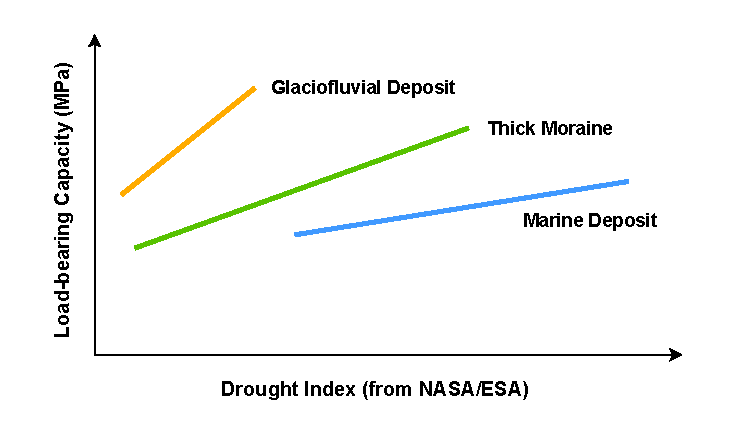
\includegraphics[width=0.7\linewidth]{figures/bæreevne_tørkeindex.pdf}
    \caption[Graph comparing load-bearing capacity to \acrshort{swi}]{Graph comparing load-bearing capacity to \acrshort{swi}, recreated from the task description [\hyperref[appendix:task_description]{Appendix \ref*{appendix:task_description}}]}
    \label{fig:load_to_swi_graph}
\end{figure}

While these studies highlight the feasibility of digital road classification, practical solutions for transport managers remain limited. Current industry practices often rely on experience-based assessments and manual planning, leading to inefficiencies and uncertainty. Although some digital tools have been developed to assist in forest road accessibility assessment, they are not universally applicable across different regions.

\section{Existing Solutions}
% Hva gjør transportledere nå? (spørsmål til usertesting maybe?)

One example is Harvester Seasons\footnote{\url{https://harvesterseasons.com/}}, developed by the Finnish Forest Center, which provides weekly forecasts of road conditions based on soil moisture, temperature, and snow depth. These forecasts use data from sources like \acrshort{nasa}'s \gls{smap} and \acrshort{esa}'s \Gls{sentinel-1} satellites to generate relative load-bearing predictions for winter and snow-free seasons [\hyperref[appendix:task_description]{Appendix \ref*{appendix:task_description}}]. While this tool offers valuable insights, it is limited to Finland and does not provide road condition data for Norway. As a result, it does not meet the needs of Skogkurs, which requires a solution tailored to Norwegian forest roads. This highlights the gap in available tools and the need for a localized approach that accounts for Norway’s specific terrain, climate, and forestry infrastructure.

The current process of scheduling operations for transport managers is based on weather conditions and road \gls{trafficability}. They plan operations either by necessity (e.g., during wet conditions) or by opportunity (e.g., in dry conditions). These decisions are informed by temperature-driven seasonality, regional precipitation patterns, and local knowledge. Additionally, transport lead times and road conditions are influenced by surface deposits and their \gls{permeability}, with difficult weather and reduced road \gls{trafficability} being major challenges in wood supply and transport management \cite{fjeld2023trafficability}. 

\section{Framework}

\textcolor{orange}{NOE TEKST}

\section{Project Organization}

\textcolor{orange}{NOE TEKST}

\section{Thesis Structure}

\textcolor{orange}{NOE TEKST}

\chapter{Requirements}\label{chap:requirements}

\textcolor{orange}{NOE TEKST}

This chapter presents the requirements provided the \gls{productowner}

This chapter presents a reflection on both the development process and the final product. It examines how the project evolved in relation to the original goals, highlighting what worked well, what could have been improved, and the challenges encountered along the way. The chapter discusses the choice of technologies, project management practices, and team collaboration. It also evaluates the effectiveness and limitations of the final solution, comparing it with existing alternatives and identifying unexpected findings. Broader considerations, such as sustainability and the role of AI in the project, are explored. Finally, the chapter outlines potential directions for future work and improvements to both the product and the project approach.


\section{Project Goals}

This section outlines the overall goal of the project, categorized into product goals, impact goals, and learning goals. Together, these objectives defines the purpose, intended outcomes, and the knowledge expected to be gained through the project process.

\subsection{Product Goals}\label{subsec:req:productgoals}

The primary goal of the project is to develop and test a \textbf{prototype system for fully digital modeling of forestry road load-bearing capacity under varying conditions throughout the year.} The solution will incorporate various geological and meteorological parameters, such as soil type and moisture, weather forecasts, and precipitation data, to generate an accurate classification of forest roads. This classification will be presented through an interactive map-based website. Furthermore, the system will prioritize ease of use, with an intuitive interface designed for transport managers, allowing them to make informed route choices based on real-time data and forecasts. 

\textcolor{orange}{DETTE UNDER ER IKKE NØDVENDIG HER}
The roads will be color-coded using a traffic-light system, where green indicates safe roads, yellow signals caution, and red highlights unsafe roads. The system will provide users with a forecast for road conditions at least a week into the future, enabling better planning and decision-making. 

\subsection{Impact Goals}\label{subsec:req:impactgoals}
% Bærekraft ?
\begin{itemize}
    \item Reduced uncertainty for transport managers when setting the routes using forest roads.
    \item To validate the prototype's feasibility and effectiveness by conducting tests with end-users, such as transport managers, to assess its performance and usability in real-world scenarios.
\end{itemize}

\subsection{Learning Goals}\label{subsec:req:learninggoals}
% Kanskje korte ned litt på dette
% Kanskje oppdatere med noe nytt?? WMS, GIS, osv.
\begin{itemize}
    \item Gaining insight in implementing interactive maps and geospatial data on web pages.
    \item Leveraging RESTful APIs for efficient data integration.
    \item Acquiring hands-on experience collaborating with real-world companies and products.
    \item Gaining experience working in a team environment, improving collaboration and communication skills.
    \item Conducting user tests and implementing feedback. 
    \item Developing a deeper understanding of the software development life cycle while actively practicing agile methodologies, like Scrum and Kanban.
    \item Enhancing application performance by implementing concurrency and optimizing parallel processing.
    \item Expanding proficiency in containerization techniques, particularly through hands-on experience with Docker.
    \item Implementing \Gls{openstack} deployment and configuration using Terraform for efficient infrastructure management.
    % Ikke ta med fra NTNU, heller referer
    \begin{comment}
    \item \textit{\textbf{From NTNU \cite{ntnu_idatg2900}:}}
    \begin{itemize}
        \item Has in-depth knowledge of a selected topic within the subject area.
        \item Has knowledge of research and development work within the topic.
        \item Can identify, formulate and solve a relevant engineering problem.
        \item Can apply knowledge and relevant results from research and development work to solve theoretical, technical and practical problems within the topic of the bachelor thesis and justify their choices.
        \item Can apply engineering methods and work methodically.
        \item Can document and disseminate engineering work.
        \item Can plan and carry out engineering work.
        \item Disseminates professional knowledge to various target groups both in writing and orally in Norwegian and English.
        \item Has insight into scientific honesty and understanding of ethical issues.
        \item Has insight into environmental, health, social and economic consequences of products and solutions within their field and can put these in an ethical perspective and a life cycle perspective.
        \item Integrates previously acquired knowledge and is able to acquire new knowledge in solving a problem.
    \end{itemize}
    \end{comment}
\end{itemize}

\section{Constraints}

\textcolor{orange}{NOE TEKST}

\subsection{Temporal Constraints}

\textcolor{orange}{NOE TEKST}

\begin{itemize}
    \item The set deadline for the final report is 20th of May.
    \item The presentation of the bachelor's thesis is scheduled for 4th or 5th of June.
\end{itemize}

\subsection{Product Constraints}

\textcolor{orange}{NOE TEKST}

\begin{itemize}
    \item The product requires a stable network connection to be used.
    \item The product uses \acrshort{html} 5, which requires newer versions of browsers.
    \item The product needs to be deployed either locally or on a server to run.
\end{itemize}

\begin{comment}
    \subsection{Legal Constraints}
% VET IKKE OM DETTE SKAL VÆRE MED
% ENDRE TIL NÅTID (THE PRODUCT COMPLIES WITH....) ?
\begin{itemize}
    \item The product must comply with the licensing terms and conditions of all third-party services, including map distributors, external APIs, and any code libraries, frameworks, or tools used in its development and deployment.
\end{itemize}
\end{comment}

\section{Project Tasks}
% VET IKKE OM DETTE SKAL VÆRE MED (KANSKJE FJERNE DELER ELLER PEK TIL PROSJEKT PLANEN)
The project aims to develop and test a prototype system for fully digital modeling of forest road load-bearing capacity under varying conditions throughout the year. The development process can be divided into the following areas:

\begin{enumerate}
    \item \textbf{Data Collection and Integration:}
    \begin{itemize}
        \item Decide and gather relevant geological and meteorological data, which may include:
        \begin{itemize}
            \item Superficial deposits, soil moisture, ground water, ground frost.
            \item Weather forecasts.
            \item Historical and real-time road conditions.
        \end{itemize}
        \item Identify and implement suitable data sources and APIs for continuous updates.
    \end{itemize}
    
    \item \textbf{Classification and Forecasting:}
    \begin{itemize}
        \item Develop a rule-based model to classify road conditions based on environmental factors.  
        \item Implement a traffic-light classification system (Green = Safe, Yellow = Caution, Red = Unsafe).  
        \item Extend the model to provide forecasted road conditions at least a week in advance.  
    \end{itemize}
    
    \item \textbf{Web-Based Visual and User Interface:}
    \begin{itemize}
        \item Design and develop an interactive map-based website for intuitive accessibility.
        \item Implement a GIS-based visualization with real-time updates and historical road condition tracking. 
        \item Ensure that the system is optimized for transport managers, with a user-friendly interface that allows efficient decision-making. 
    \end{itemize}
    
    \item \textbf{Testing, Validation and Refinement}:
    \begin{itemize}
        \item Evaluate the accuracy and usability of the system by testing with real-world data.
        \item Conduct user testing with transport managers or forestry stakeholders to assess the effectiveness of the interactive interface and forecasting capabilities.
        \item Incorporate potential user feedback.
    \end{itemize} 
    
    \item \textbf{Documentation and Future Work:}
    \begin{itemize}
        \item Provide detailed documentation of the system architecture, data sources, and model.
        \item Provide a detailed user guide of the product.
        \item Suggest potential improvements, such as machine learning model enhancements, additional data sources, mobile application integration, optimization, or further improvements of the app interface.
    \end{itemize}
\end{enumerate}

\section{Target Audience}

The primary target audience for this application is transport managers in the Norwegian forestry industry. They will use the application to plan routes and determine which forest roads should be used by drivers. Since the user group spans a wide age range, it is essential that the application is intuitive and easy to use, ensuring accessibility for all users regardless of their technical proficiency.

\section{Universal Design}

\textcolor{orange}{NOE TEKST}
\begin{comment}
    Kanskje ikke nødvendig med eget kapittel og kanskje ha det et annet sted? Passer med overgang fra Target Audience ^. SIDEN NOE OM DETTE IKKE BLE NEVNT AV SKOGKURS SÅ BURDE DET KANSKJE STÅ I DISCUSSION I STEDET.
\end{comment}

\section{Use Case}

Use cases provide a clear overview of what a system will and will not do. They enable effective scope management and incremental development, making them well-suited for agile methodologies \cite{jacobson_use_case}. 

This section will present the use case diagram of the system and provide an example of a use case specification.

\subsection{Use Case Diagram}
% DOBBELSJEKK AT SERVEREN IKKE SKAL KOBLES TIL USE CASENE I DIAGRAMMET
The use case diagram shows all interactions the user will have with the website. It also features the application server and its relationship with the external map servers.
\begin{figure}[h]
    \centering
    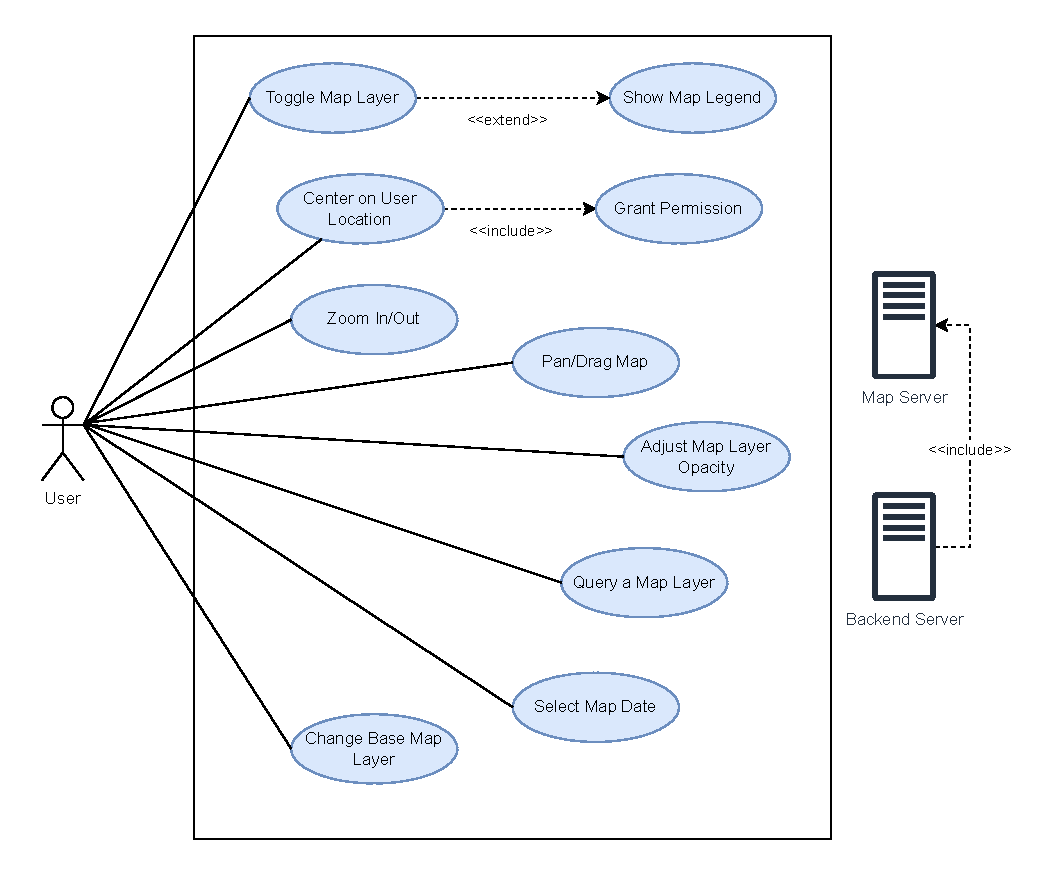
\includegraphics[width=1\linewidth]{figures/use_case_diagram.pdf}
    \caption{Use case diagram of system}
    \label{fig:use_case_diagram}
\end{figure}

\subsection{Actors}

\begin{itemize}
    \item \textbf{User:} The primary user of the website, typically transport managers in the forestry industry, who interact with the system to access relevant map and logistics data.
    \item \textbf{Backend Server:} The central server that the website communicates with to retrieve all necessary map data. It aggregates, processes, and refines data from external services before delivering it to the website.
    \item \textbf{Map Server:} External services that provide map data, either through a \Gls{wms}, \Gls{wfs}, or an \acrshort{api}, which the backend server integrates into the system.
\end{itemize}

\subsection{Use Case Specifications}

It is important to show how users interact with the system to achieve their goals. The use case specifications provide details of each use case and the basic path the user takes to achieve their goals while also capturing possible exceptions. 

A high priority use case for the website is the ability to toggle a map layer, which allows users to control the visibility of different layers. The use case specification for this functionality is shown in \hyperref[tab:use_case_toggle_layer]{Table \ref*{tab:use_case_toggle_layer}}. Additional use case specifications for other features can be found in \hyperref[appendix:use_case_specifications]{Appendix \ref*{appendix:use_case_specifications}}.

\begin{table}[h]
    \centering
    \begin{tabularx}{\textwidth}{|l|X|}
        \hline
        \rowcolor{gray!20}
        \textbf{Use Case Name} & Toggle Map Layer \\
        \hline
        \textbf{Actor(s)} & User \\
        \hline
        \textbf{Description} & The user can toggle specific map layers to control the visibility of different map layers. This functionality allows users to select from various map layers. The selected layer is then displayed, and relevant information is shown in the map legend sidebar. \\
        \hline
        \textbf{Priority} & High \\
        \hline
        \textbf{Pre-Condition(s)} & The user must have a stable internet connection and the website open. The website, server and external map servers must be deployed and running.\\
        \hline
        \textbf{Post-Condition(s)} & The map will be updated with the specific map layer that was toggled. The map legend will also be visible in the legend sidebar. \\
        \hline
        \textbf{Basic Path} &  
        \begin{enumerate}[label=,left=0pt]
            \item 1. User presses the map layer ("kartlag") button to open the map layer sidebar.
            \item 2. User clicks the toggle button for the specific map layer to toggle.
            \item 3. The system updates the map with the selected layer.
        \end{enumerate} \\
        \hline
        \textbf{Exception Path} & 
        \begin{enumerate}[label=,left=0pt]
            \item 0. User does not have a stable internet connection and can not connect to the website.
            \item 2a. Either the backend server or the map server is not responding, and no map data is received.
        \end{enumerate} \\
        \hline
    \end{tabularx}
    \caption[Use Case Specification: Toggle Map Layer]{Use case for toggling a map layer}
    \label{tab:use_case_toggle_layer}
\end{table}

\chapter{Technical Design}\label{chap:technicaldesign}

\begin{comment}
    # Universal Design (Universal Utforming)
    # OpenLayers vs Leaflet (or others)
    # Openlayers TileWMS vs ImageWMS (optimalisering av kartet)
\end{comment}
\textcolor{orange}{NOE TEKST}

\section{System Architecture}\label{sec:systemarchitecture}

% client-server model, microservices, layers of the application ? 
\textcolor{orange}{NOE TEKST}

\section{Data Flow} % e.g., how user requests move through the system).

\textcolor{orange}{KANSKJE TEMP LOKASJON}

\section{Sequence Diagram}
\begin{figure}[h]
    \centering
    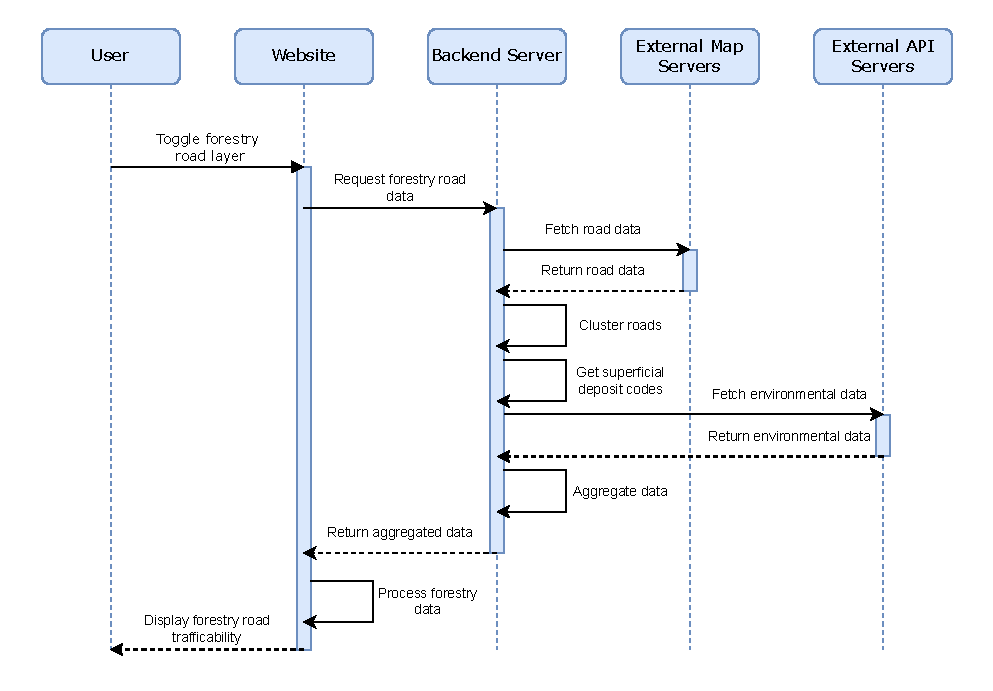
\includegraphics[width=1\linewidth]{figures/sequence_diagram.pdf}
    \caption{Sequence diagram of forestry road map layer}
    \label{fig:sequence_diagram}
\end{figure}

\hyperref[fig:sequence_diagram]{Figure \ref*{fig:sequence_diagram}} shows the sequence diagram for when the user toggles the forestry road map layer. The whole sequence consists of these steps:
\begin{enumerate}
    \item \textbf{Toggle forestry road layer}: The user toggles the forestry road map layer on the website.
    \item \textbf{Request forestry road data}: The website sends a request to the backend server for the necessary data within the visible map area.
    \item \textbf{Fetch road and weather data}: The backend server, acting as a proxy, fetches the required road and weather data from external map servers.
    \item \textbf{Return road and weather data}: The map servers return the requested road and weather data.
    \item \textbf{Aggregate data}: The backend server aggregates the data into a single payload.
    \item \textbf{Return aggregated data}: The backend server sends the aggregated data back to the website.
    \item \textbf{Process forestry data}: The website processes the data and determines the trafficability of roads within the visible map area.
    \item \textbf{Display forestry road trafficability}: The forestry road layer, including trafficability, is rendered on the user's map.
\end{enumerate}

\section{Website}

The website serves as the user interface of the system, allowing users to visualize and interact with data related to forestry road conditions and weather-based forecasts using a dynamic map.

The system follows a client-server architecture, where the website acts as a client and communicates with a backend server via a REST API. The processing of meteorological and geological data is handled on the server side. The frontend is responsible for requesting data, rendering maps, and presenting relevant information to the user.

The classification of road trafficability is performed on the client side, as the website allows users to dynamically adjust thresholds for certain meteorological and geological parameters. Normally, this would be handled entirely by the backend server, but in order to provide immediate feedback when the user changes these thresholds, the classification logic is implemented in the frontend. This hybrid approach ensures a responsive user experience while keeping the most computationally expensive operations on the server.

The interaction between the website and the server is stateless, meaning that each request is independent and contains all the information needed to process it. This architectural choice improves system robustness and simplifies both development and deployment, particularly when it comes to scaling.

A central component of the website is its interactive map interface, which displays spatial data such as forestry road networks, map layers, and calculated trafficability classifications. The map is rendered dynamically in the browser using client-side resources, and data is loaded based on the user’s current viewport and zoom level. This approach ensures efficient data usage and good performance, even when dealing with large or detailed geographic datasets.

The website is implemented as a single-page application (SPA), where all rendering and interface updates occur dynamically without full page reloads. This enables smooth interaction and better performance, as only relevant parts of the page are updated via the Document Object Model (DOM). \acrshort{html} 5 is required for full functionality, and the system relies on an active internet connection to fetch data from the server and external services. While the system is primarily intended for desktop and laptop use, it also runs on mobile devices, though the \acrshort{ui} is not optimized for smaller screens.

Choosing to implement the frontend as a web application provides several benefits. It ensures accessibility across a wide range of devices without the need for local installation, making the tool usable both in office environments and in the field.

Overall, the design of the website emphasizes a clean separation of concerns, efficiency in data handling, and accessibility, which together form a robust and user-friendly frontend component for the system.

\subsection{Road Classification}

\textcolor{orange}{
Blablabla noe \autoref{fig:forestryroadclassification}
}

\begin{figure}[h]
    \centering
    \centerline{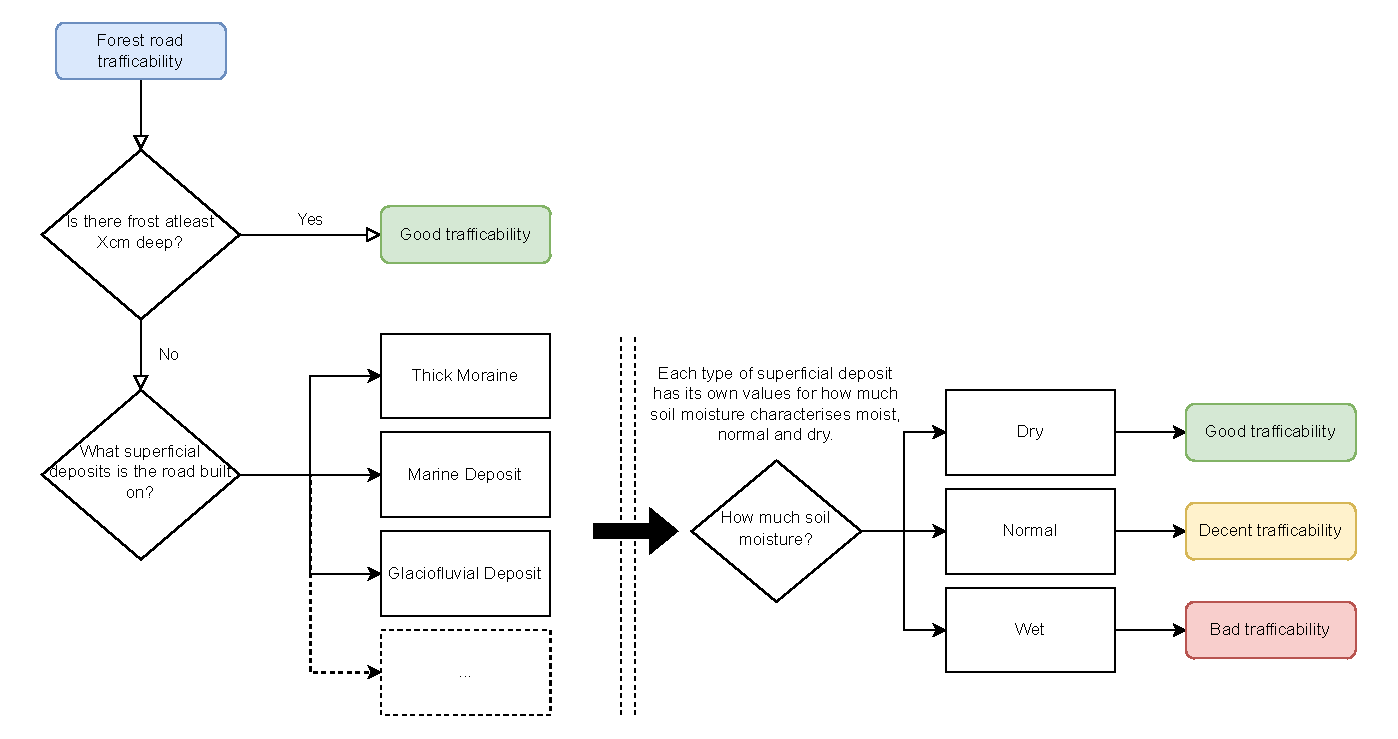
\includegraphics[width=1.2\linewidth]{figures/roadclassification.pdf}}
    \caption{Diagram visualizing the forestry road classification}
    \label{fig:forestryroadclassification}
\end{figure}

\subsection{Folder Structure}

\textcolor{orange}{NOE TEKST}
\begin{figure}[h]
    \centering
    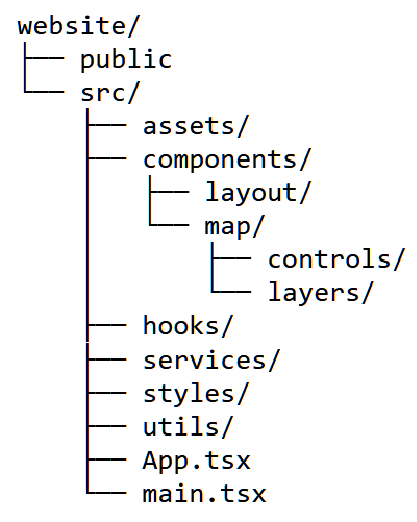
\includegraphics[width=0.5\linewidth]{figures/website_folder_structure.pdf}
    \caption{Folder structure of the website}
    \label{fig:website_folder_structure}
\end{figure}

\section{Server}

\textcolor{orange}{NOE TEKST}

\subsection{Forestry Road Processing}

\subsection{Proxy}


% Multiple map services were used in this project to ultimately determine the trafficability of forestry roads. Retrieving data from WMS and WFS was made easy with OpenLayers as it includes functions for this. 


\subsection{Folder Structure}



% ANDRE DIAGRAM? sequence diagrams, component diagrams, etc.
\chapter{Map Data Sources}

\textcolor{orange}{NOE TEKST}

\section{Map Layers}

% KANKJE GLOSSARY FOR "COMPOSITE MAP"
The interactive map on the website supports multiple layers, allowing the user to build a composite map with various types of data. These layers include both meteorological and geological data relevant to assessing road conditions and the surrounding environment.

\subsection{Base Layers}

The user has the option to change the base layer of the map. In the current version, two options are available: the standard map from \Gls{openstreetmap}\footnote{\url{https://www.openstreetmap.org}} and the terrain map from OpenTopoMap\footnote{\url{https://opentopomap.org}}.
% KANSKJE GI GRUNN TIL HVORFOR DET IKKE KUN ER ETT BASE LAYER VALG

\begin{figure}[h]
     \centering
     \begin{subfigure}[b]{0.45\textwidth}
         \centering
         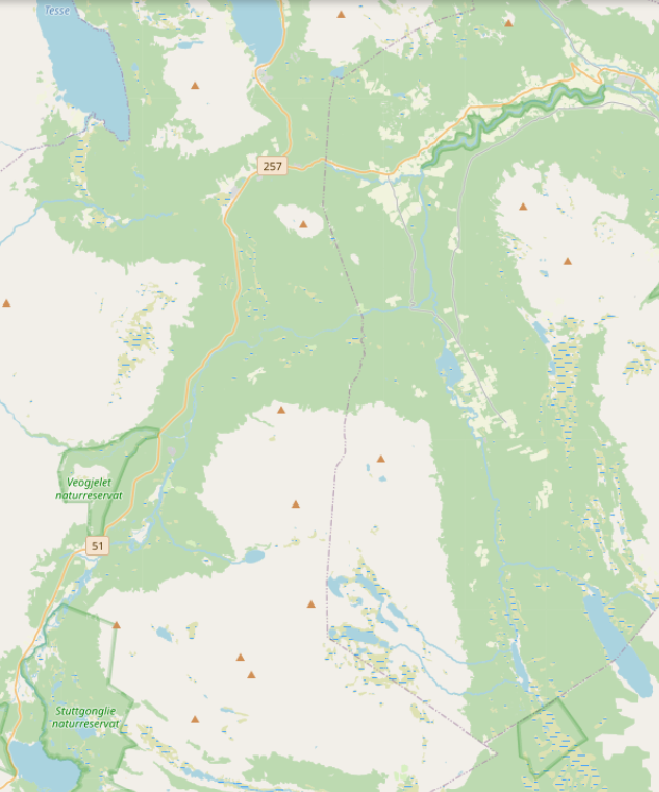
\includegraphics[width=\textwidth]{figures/base_layer_standard.pdf}
         \caption{Standard base layer}
         \label{fig:base_layer_standard}
     \end{subfigure}
     \hfill
     \begin{subfigure}[b]{0.45\textwidth}
         \centering
         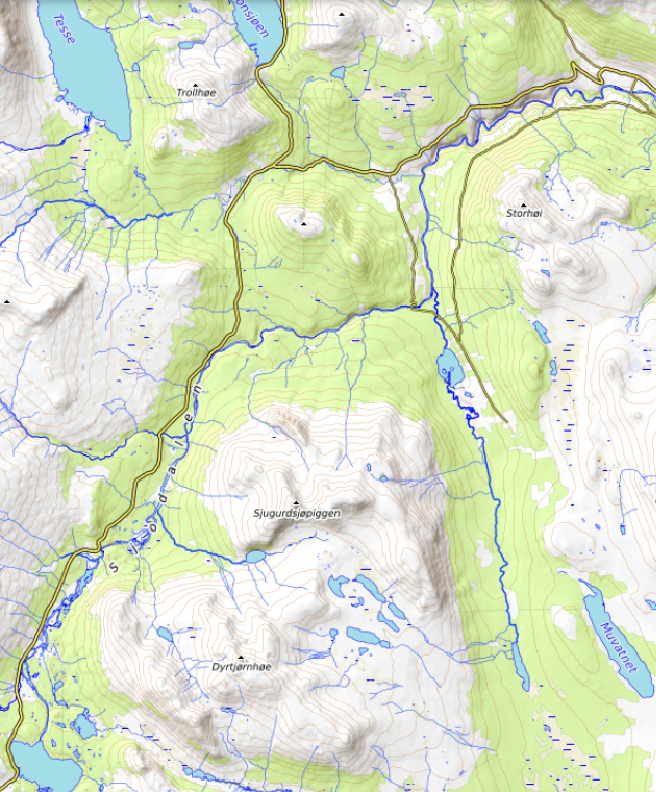
\includegraphics[width=\textwidth]{figures/base_layer_topo.pdf}
         \caption{Terrain base layer}
         \label{fig:base_layer_topo}
     \end{subfigure}
    \caption{Base map layer options}
    \label{fig:base_layers}
\end{figure}

\subsection{Superficial Deposits}
% LEGGE INN FARGE KODER FOR LØSMASSETYPE. TRENGER IKKE FOR ALLE? KANSKJE VEDLEGG?
The map layer showing superficial deposits is provided by \acrshort{ngu}. The superficial deposits data provide information on the distribution of surface sediments covering bedrock, mainly formed during and after the last Ice Age. It represents the dominant soil type in the upper layers, but does not account for deeper variations. These soil types include stones, gravel, sand, clay, peat, and moraine material \cite{geonorge_losmasser}. 

\begin{figure}[h]
    \centering
    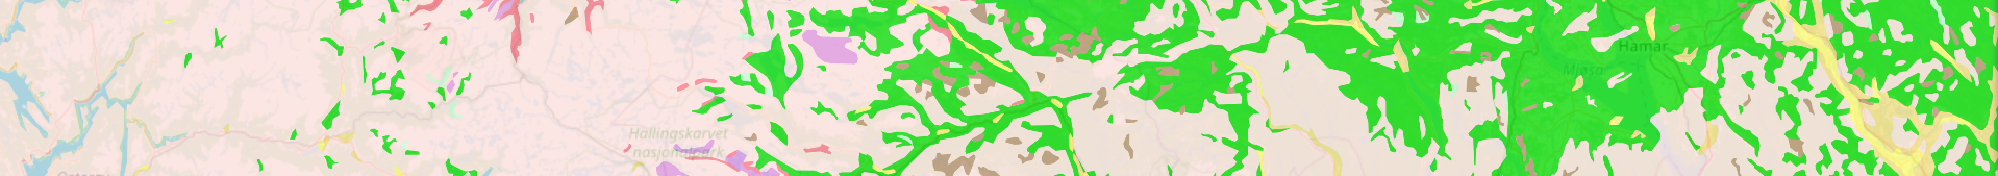
\includegraphics[width=1\linewidth]{figures/losmasse_eksempel.pdf}
    \caption{Example of the superficial deposits map layer}
    \label{fig:superficial_deposit_example}
\end{figure}

\subsection{Frost Depth}

% Kanskje nevn GWB modellen? https://www.senorge.no/WaterMap
% TODO: DOBBELSJEKK AT VI SKAL BRUKE 10CM FOR TELE
The frost depth map layer, provided by \acrshort{nve}, visualizes frost depth as a raster map, with colors ranging from dark blue (indicating deep frost) to light green (indicating no frost). This layer is particularly useful for assessing the trafficability of forestry roads. When frost depth reaches 10 cm or more (see \hyperref[tab:frost_depth_classification]{Table~\ref*{tab:frost_depth_classification}}), road conditions are generally suitable for heavy vehicles. As a result, most forestry roads tend to have good trafficability throughout the Norwegian winter, when frost is typically present.

% KANSKJE GI EKSEMPLER PÅ NÅR (OG HVOR) DET ER VANLIG MED DE FORSKJELLIGE DYBDENE
\begin{table}[h]
    \centering
    \begin{tabular}{|l|l|l|}
        \hline  
        \textbf{Color} & \textbf{Frost Depth} & \textbf{Depth in cm} \\
        \hline
        \cellcolor[HTML]{00009c} & Very Deep Frost & > 75 cm \\
        \hline
        \cellcolor[HTML]{0018ff} & Deep Frost & 30-75 cm \\
        \hline
        \cellcolor[HTML]{009aff} & Frost & 10-30 cm \\
        \hline
        \cellcolor[HTML]{84ebff} & Shallow Frost & 5-10 cm \\
        \hline
        \cellcolor[HTML]{deffff} & Partially Frost-free & 0-5 cm \\
        \hline
        \cellcolor[HTML]{cef77b} & No Frost & 0 cm \\
        \hline
    \end{tabular}
    \caption{Frost depth classification and corresponding colors \cite{nve2025waterdata}}
    \label{tab:frost_depth_classification}
\end{table}

\begin{figure}[h]
    \centering
    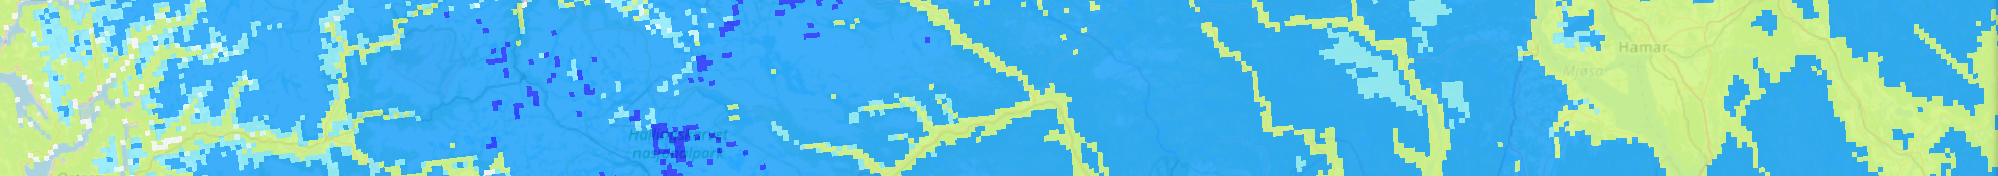
\includegraphics[width=1\linewidth]{figures/teledyp_eksempel.pdf}
    \caption{Example of the frost depth map layer}
    \label{fig:frost_depth_example}
\end{figure}

\subsection{Soil Saturation}

% Glossary groundwater & root zone
The soil saturation data, provided by NVE, represents the ratio between the current simulated water content in the groundwater and root zone and the highest value observed during the historical reference period from 1981 to 2010 \cite{nve2025waterdata}. For example, a soil saturation level of 70\% indicates that the soil currently holds 70\% of the maximum water content recorded during that period.

Soil saturation can be used to assess \gls{trafficability}, which refers to the highest level of soil moisture a road can tolerate without experiencing unacceptable deformation. This threshold varies depending on the type of superficial deposits present, as different materials have varying levels of permeability \cite{fjeld2023trafficability}.

\begin{table}[h]
    \centering
    \begin{tabular}{|l|l|}
        \hline  
        \textbf{Color} & \textbf{Soil Saturation (\%)} \\
        \hline
        \cellcolor[HTML]{f82200} & Above 90\% \\
        \hline
        \cellcolor[HTML]{f8c400} & 80 - 90\% \\
        \hline
        \cellcolor[HTML]{f8fc00} & 70 - 80\% \\
        \hline
        \cellcolor[HTML]{29d460} & 60 - 70\% \\
        \hline
        \cellcolor[HTML]{e4e4e4} & Under 60\% \\
        \hline
    \end{tabular}
    \caption{Soil saturation classification and corresponding colors \cite{nve2025waterdata}}
    \label{tab:soil_saturation_classification}
\end{table}

\subsection{Forestry Roads}

The forestry roads map layer is a vector dataset retrieved via a WFS service in GeoJSON format, provided by GeoNorge and Kartverket. In the GeoJSON, forestry roads are represented as geometric LineString features, where each LineString defines a segment between two coordinates. A single road is often divided into multiple such features. The GeoJSON also includes properties of each features such as road number, municipality number, and feature length.

\textcolor{orange}{Skrive om at implmenetation kommer senere, men nevne korte trekk hva layeret er.}

\section{Gridded Water Balance Model}

The Gridded Water Balance (GWB) model is responsible for calculating the hydrological variables shown in the SeNorge\footnote{\url{https://www.senorge.no}} grid maps. It is a spatially distributed adaptation of the HBV model, which was initially designed for flood forecasting, and it calculates water balance for each \qty{1}{\kilo\meter\squared} grid cell separately \cite{nve2025waterdata}.

Each grid cell is characterized by its average elevation and the distribution of land cover types, such as vegetation, soil, wetlands, lakes, and glaciers. The model operates on a daily time step, using spatially distributed data for temperature and precipitation as its inputs \cite{nve2025waterdata}.

GWB includes processes for snow storage, root zone moisture, groundwater storage, evaporation, runoff to rivers, wetlands, lakes, frost depth, and glaciers. Potential evaporation is calculated based on air temperature and vegetation development during the growing season, while actual evaporation is limited by the availability of soil moisture \cite{nve2025waterdata}.

Water balance calculations are conducted independently for each grid cell. The parameterization of each cell incorporates variations in topography, vegetation, and soil type, reflecting their impact on local hydrological processes \cite{nve2025waterdata}.

Both the frost depth and soil saturation map layers from SeNorge and NVE are derived using the GWB model.

\section{Sources of Uncertainty}

\textcolor{orange}{Gjerne skriv om feilkilder fra andre en senorge dataen}

Various factors contribute to uncertainties in the frost depth and soil saturation maps. These include possible errors in the interpolation of meteorological and soil data, as well as limitations in how the model translates real-world conditions. These uncertainties are especially important around the freezing point (0°C), where even minor temperature variations can influence whether precipitation falls as rain or snow, or if snow begins to melt \cite{senorge_watermap}. The frost depth map tends to provide more accurate simulations of soil freezing compared to soil thawing \cite{nve2025waterdata}.

Localized weather events, such as isolated rain showers missed by nearby weather stations, may also go unnoticed. Furthermore, environmental factors like wind, humidity, and solar radiation, which are not accounted for in the model, can speed up snowmelt, causing discrepancies between the model’s predictions and actual conditions \cite{senorge_watermap}.

The SeNorge maps show daily averages, which may miss short-term variations like intense rainfall or rapid changes in temperature within a single day. The forecast maps predict up to nine days ahead, with increasing uncertainty the further into the future the prediction extends. Finally, the model's representation of vegetation and soil types may not always be accurate, potentially leading to the overestimation or underestimation of soil saturation levels \cite{senorge_watermap}.
\chapter{Development Process}\label{chap:developmentprocess}

\textcolor{orange}{NOE TEKST}

\section{Code Repositories}

% Github Organization and repos
All code and project-related resources are stored on GitHub under a dedicated organization\footnote{\url{https://github.com/skogkursbachelor}}. Each component of the system, as well as supporting documentation, is maintained in its own repository. This modular structure facilitates collaboration and version control throughout the development process.

An overview of the repositories and their respective purposes is shown in \autoref{tab:githubrepositories}.

\begin{table}[h]
    \centering
    \begin{tabular}{l|l}
        \hline
        \textbf{Repository} & \textbf{Description} \\
        \hline
        server & The code for the backend server. \\
        website & The code for the website. \\
        \hline
        meetingminutes & Collection of meeting minutes. \\
        diagrams & Collection of draw.io\tablefootnote{\url{https://www.drawio.com/}} diagrams. \\
        \hline
        thesis & A backup version of the thesis. \\
        projectplan & A backup version of the project plan. \\
        \hline
    \end{tabular}
    \caption[Overview of GitHub repositories]{Overview of GitHub repositories\tablefootnote{\url{https://github.com/orgs/skogkursbachelor/repositories}}}
    \label{tab:githubrepositories}
\end{table}

\section{Backup Server}

Blabla found in \autoref{lst:backupserverls}.

\begin{figure}[h]
\lstinputlisting[
    caption={Files on the backup server},
    label=lst:backupserverls,
    language=bash
]{listings/backupserver.txt}
\end{figure}

\textcolor{orange}{
Refere til 3-2-1 backup strategy hvis vi skriver om det her, hvertfall i project plan \\ \\
Hvordan det blir deployed \\ \\
Hvordan backupene skjer, crontab + git
}

\section{Time Tracking}

All project work was tracked using the self-hosted time tracking service Traggo\footnote{\url{https://traggo.net/}}. Traggo tracks work by tags making it easy to get an overview of time spent on different tasks.

\begin{table}[h]
    \centering
    \begin{tabular}{c|c|c|c}
        \hline
        \textbf{Month} & \textbf{Bjørnsen} & \textbf{Houmb} & \textbf{Total} \\
        \hline
        January  & 61h 39m  & 62h 58m  & 124h 37m \\
        February & 80h 6m   & 79h 17m  & 159h 24m \\
        March    & 88h 4m   & 88h 20m  & 176h 24m \\
        April    & 99h 40m  & 102h 38m  & 202h 18m \\
        May      &        &        &        \\
        \hline
        Total & & & \\
        \hline
    \end{tabular}
    \caption{Tracked time by month and group member}
    \label{tab:timetrackedbymember}
\end{table}

% Skriv mer om time fordeling, f.eks. hvorfor mer timer i mars enn januar etc.
\autoref{tab:timetrackedbymember} shows the total time of work for each month by the two members.

% KANSKJE IKKE TA SKJERMBILDE, LAG HELLER CHART MED LATEX f.eks. (pfg-pie).
\begin{figure}[h]
    \centering
    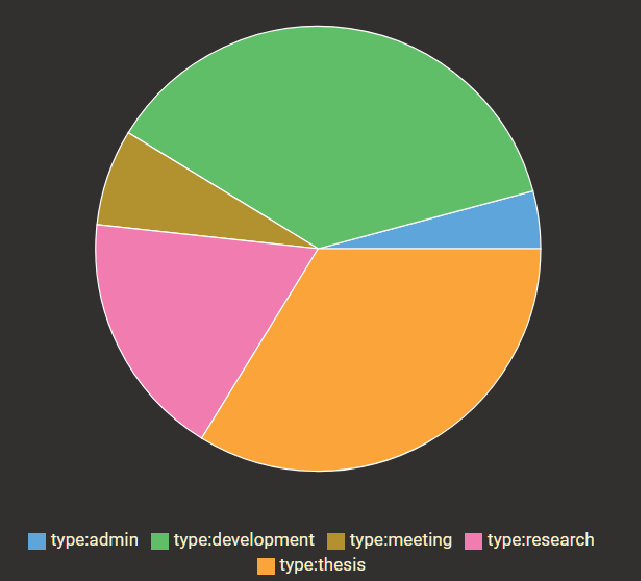
\includegraphics[width=0.5\linewidth]{figures/time_tracking_by_type.pdf}
    \caption{Pie chart of time spent in total per work type}
    \label{fig:time_tracking_by_type}
\end{figure}

% SKRIV OM TIDSFORDELING FOR DE FORSKJELLIGE OPPGAVENE (THESIS, DEV, osv.)

\section{Work Allocation}

\textcolor{orange}{Kanskje ta dette med? Hvordan utviklingsjobben for forskjellige deler av system ble tildelt?}

\section{Gantt Diagram}

A Gantt chart was created, highlighting the different sprints and key milestones. It served as a high-level plan to structure the project's progression but was not intended to be followed rigidly, allowing for flexibility and adjustments along the way, which is particularly important in agile development projects. This approach provided a clear visual overview for team coordination and progress tracking. A more detailed table of all dates referenced in the Gantt chart can be found in the project plan (see \autoref{appendix:project_plan}).

\begin{figure}[h]
    \centering
        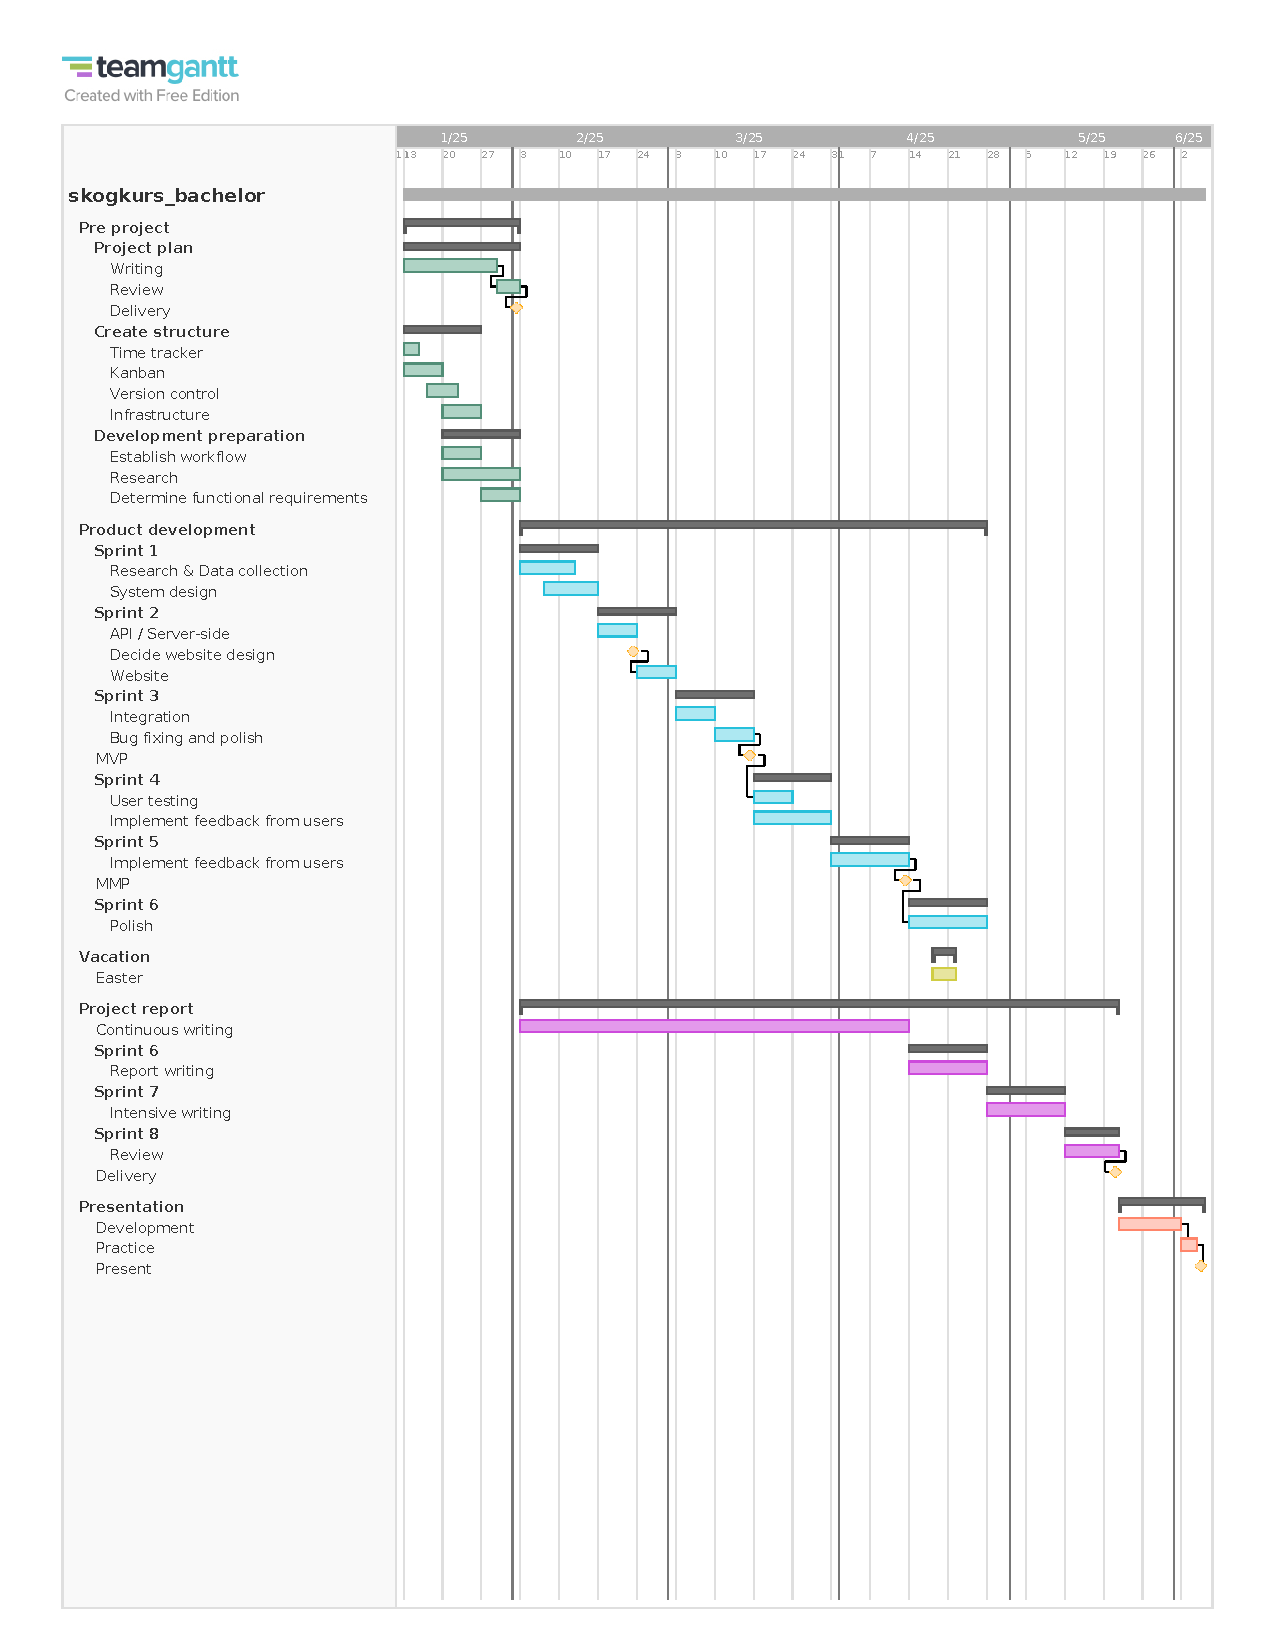
\includegraphics[width=1.0\linewidth, trim=0 60mm 0 20mm, clip]{figures/skogkurs_bachelor_gantt.pdf}
    \caption{Gantt diagram of the project}
    \label{fig:gantt_diagram}
\end{figure}

\section{Software Development Lifecycle Model}

For this project, the team needed to select an appropriate \acrfull{sdlc} model. Key factors considered in this decision included the clarity and flexibility of the requirements, team size, project timeline, product delivery goals, and prior experience \cite{sdlc_model}. 

The requirements provided by the Product Owner are intentionally ambiguous and flexible, allowing the team to prioritize the few fixed requirements upfront while iteratively refining the flexible ones over time. The team is composed of two members with similar experience levels, enabling close collaboration and effective decision-making. With a short project timeline of four months, a structure of 2-week sprints aligns perfectly with Scrum's iterative and adaptive approach, ensuring steady progress and regular opportunities for feedback. 

Given the absence of clearly defined requirements and the need for continuous collaboration with the Product Owner, the Scrum methodology was the most appropriate framework for managing the team’s workflow and project development. Traditional methodologies like Waterfall are not suitable, as they rely on fixed requirements and a linear development process, which would limit the teams flexibility \cite{waterfall_model_enwiki:1275499744}. Extreme Programming (XP), while valuable for high-collaboration environments with strict engineering practices like pair programming and test-driven development, is not fully suitable as the project does not emphasize these practices to the same extent \cite{extreme_programming}. Similarly, Lean development focuses on minimizing waste and maximizing efficiency but is less structured in terms of iterative planning, which is needed to manage evolving requirements effectively \cite{lean_programming}. By adopting Scrum, the team can iteratively refine requirements and adapt to changes throughout development \cite{sdlc_model}. To implement Scrum effectively, several key practices are integrated into our workflow \cite{scrum_guide}.

\begin{itemize}
    \item \textbf{Sprint Meetings:} The project is divided into 2-week sprints. At the start of each sprint, sprint meetings included sprint planning, reviews, and retrospectives. During the planning phase, the team selects tasks from the product backlog to form the sprint backlog for the upcoming sprint. The review phase focuses on evaluating progress and determining whether adjustments to the product backlog are needed. The goal of the retrospective phase is to identify areas for improvement in the Scrum process itself.
    \item \textbf{Daily Scrum Meetings:} Short daily meetings are conducted to discuss the progress of ongoing tasks, identify potential obstacles, and ensure alignment between team members. 
    \item \textbf{Scrum Master:} Given that the team consists of only two members, we have decided to share the role of Scrum Master. Both members are responsible for ensuring adherence to the Scrum framework and continuously working to improve team efficiency. This collaborative approach allows us to maintain flexibility while upholding Scrum principles throughout the project.
    \item \textbf{Kanban:} To complement Scrum and further enhance workflow visibility, a Kanban board is utilized to track and manage tasks on GitHub. The Kanban board consists of columns representing different stages of the workflow, such as Product Backlog, Sprint Backlog, In Progress, In Review, Done, and Discarded.
\end{itemize}

\section{Sprints}

\textcolor{orange}{PUTTE HVERTFALL SPRINTREFERATENE I VEDLEGG, MEN KAN SKRIVE NOE OM SPRINTS. Peke til vedlegg. Sammenlign med det som står over, ta med sprint planning, reviews og retrospective. Sprint Reviews for selve produktet, retrospectives for prossessen. Lite å snakke om på retrospektive, men var en periode med lite arbeid på bachelor på grunn av annet fag (vet ikke om det skal nevnes?)}
% peke til vedlegg
% Sammenlign med det som står over, ta med sprint planning, reviews og retrospective

\textbf{Sprint 1}
\begin{itemize}
    \item Research & data collection
    \item System design
\end{itemize}

\textbf{Sprint 2}
\begin{itemize}
    \item API / Server-side
    \item Decide website design
    \item Website
\end{itemize}

\textbf{Sprint 3}
\begin{itemize}
    \item Integration
    \item Bug fixing and polish
    \item MVP
\end{itemize}

\textbf{Sprint 4}
\begin{itemize}
    \item User testing
    \item Implement feedback from users
\end{itemize}

\textbf{Sprint 5}
\begin{itemize}
    \item Implement feedback from users
    \item MMP
\end{itemize}

\textbf{Sprint 6}
\begin{itemize}
    \item Polish of code
    \item Report Writing
\end{itemize}

\textbf{Sprint 7}
\begin{itemize}
    \item Intensive writing
\end{itemize}


\textbf{Sprint 8}
\begin{itemize}
    \item Final review of the report
\end{itemize}

For more details about each sprint, the meeting minutes from each sprint meeting can be found in \autoref{appendix:sprint_meetings}.

\section{Meetings}

In addition to internal sprint meetings, the team held regular meetings with both the Supervisor and the Product Owner. Weekly meetings with the Supervisor offered opportunities to ask questions, receive technical guidance, and get constructive feedback, both on the product and the written report.

Meetings with the Product Owner were held on an as-needed basis rather than at fixed intervals. Most of these meetings were conducted digitally via Microsoft Teams. They were particularly valuable for clarifying requirements, discussing design decisions, and showcasing progress through product demos.

Minutes from all meetings with the Supervisor and the Product Owner can be found in \autoref{appendix:meeting_minutes}.

\section{Minimum Viable Product}

A Minimum Viable Product (\acrshort{mvp}) is a concept that focuses on learning about customers with minimal effort. An \acrshort{mvp} is an early version of a product designed to test whether customers will use or buy it, often taking the form of a simple prototype, landing page, or manually operated service. The key benefit of an \acrshort{mvp} is that it allows teams to validate ideas early, minimizing wasted effort on products that may not succeed \cite{agile_alliance_mvp}. 

\textcolor{orange}{BLE IKKE NOE MMP. Skrev om under litt: user testing -> reviews med PO, fjernet "Further details about the user testing process and findings are discussed in a later chapter."}

During the development of the website, we conducted reviews with the Product Owner to gain insights into how the target audience (transport managers) would interact with the product and identify any missing features or necessary improvements. For the \acrshort{mvp}, we prioritized implementing the core functionalities users would need, as illustrated in the use case diagram in \autoref{fig:use_case_diagram}.

\section{Minimum Marketable Product}

A Minimum Marketable Product (\acrshort{mmp}) is the next step after an \Gls{mvp} in product development. While an \acrshort{mvp} focuses on testing assumptions and user preferences, an MMP includes essential features that meet customer needs, provide a good user experience, and generate business value. It is designed to launch quickly with must-have functionality, avoiding unnecessary features that add complexity without value. The MMP approach involves refining the product to only what is essential for success. Typically, teams first develop \acrshort{mvp}s to gather insights, then use these findings to build an \acrshort{mmp} ready for general release. In agile development, combining \acrshort{mvp} and \acrshort{mmp}s helps streamline product evolution while minimizing risk and unnecessary work \cite{wanner_mmp}. 

The initial plan was to conduct user testing and implement the feedback given to create a \acrshort{mmp}, but due to unforeseen circumstances this would not be created. This will be discussed later in \autoref{chap:discussion}.

\chapter{Implementation}\label{chap:implementation}

This chapter presents the practical implementation of the system, covering both the client- and server-side components. It begins with an overview of the technologies used, including TypeScript, React, OpenLayers, Go, and Docker. The structure and functionality of the website are then described, with a focus on user interface design, map integration, and communication with the backend. Finally, the server-side implementation is detailed, including the logic behind the forestry road classification algorithm, data processing, and performance optimizations. The chapter provides a technical foundation for understanding how the prototype was built and how its components work together.


\section{Technologies}

This section outlines the key technologies used in the project, explaining both their technical roles and the reasoning behind their selection. Choices were guided by factors such as development efficiency, scalability, and compatibility with the project's geospatial and web-based requirements.

\subsection{TypeScript}

TypeScript\footnote{\url{https://www.typescriptlang.org/}} is a statically typed superset of JavaScript that adds type annotations and other features to improve code quality and maintainability. While JavaScript is popular for both frontend and backend development, it lacks built-in mechanisms to express relationships between components as applications grow. This often leads to runtime errors, many of which are related to incorrect or unexpected types. TypeScript addresses these issues by providing a static type system that checks for such errors during development, before the code is executed. By catching mistakes early and offering better tooling and autocomplete support, TypeScript makes large-scale JavaScript applications easier to develop, refactor, and maintain \cite{typescript_handbook}. 

Although the team had limited prior experience with frontend web development, we aimed to use a language that was both easy to learn and valuable beyond the project, particularly given its widespread use in industry. TypeScript was therefore chosen for the website implementation. It offered full compatibility with JavaScript-based libraries such as OpenLayers and React, while also providing static typing and enhanced code reliability.

\subsection{React}\label{subsec:implementation:technologies:react}

React\footnote{\url{https://react.dev/}} is a JavaScript library designed for rendering user interfaces (UI), where elements on the screen, from buttons to images, can be broken down into small, reusable components. These components are the building blocks of React, allowing you to create, customize, and conditionally display content across your application \cite{react_component}. As an application scales, it becomes increasingly important to manage the state effectively and ensure that data flows smoothly between components. Poorly organized or redundant state can lead to bugs, so React encourages a structured approach to state management. React makes it easy to share states between components \cite{react_managing_state}. 

Using React to develop the website improved both development speed and maintainability that was especially important given the limited timeframe of the project. React's component-based architecture allowed for modular code, easier reuse of UI elements, and better separation of concerns, which contributed to a more efficient workflow.

\subsection{OpenLayers}

OpenLayers\footnote{\url{https://openlayers.org/}} is a JavaScript library used for displaying and interacting with geographic data on web maps. It provides an extensive and well documented set of tools for working with vector and raster data, supporting various formats such as \Gls{geojson}, \Gls{wms}, and \Gls{wfs}. OpenLayers allows developers to create highly customizable and interactive maps with features like layer control, coordinate projections, and dynamic styling \cite{openlayers}.

The website uses OpenLayers to render image layers for \gls{superficial deposit}s, soil moisture, and \gls{frost} depth, and display vector features like forestry roads.  

\subsection{Web Map Service and Web Feature Service}

% NEVNE SPESIFIKKE FUNKSJONER (GetFeatureInfo / GetMap) ?
Web Map Service (\Gls{wms}) and Web Feature Service (\Gls{wfs}) are both standards developed by the Open Geospatial Consortium to facilitate the distribution of geographic information over the web. A WMS generates dynamic maps from spatially referenced data, rendering them as digital images in formats such as PNG, GIF, and JPEG. WMS allows users to request maps that specify geographic regions, desired coordinate systems, and map dimensions. There are also queryable WMS services that enable users to retrieve metadata about the map and its features at specific coordinates. Additionally, \Gls{wms} supports the creation of composite maps by layering different map images, with transparency in formats like PNG and GIF, allowing the underlying maps to be visible \cite{ogc2006wms}.

In contrast, a \Gls{wfs} enables the retrieval of raw geographic data, such as vector features, from a web server. Unlike \Gls{wms}, which provides static map images, \Gls{wfs} allows users to request feature-level data in formats like \Gls{geojson}, enabling more interactive and detailed analyses. \Gls{wfs} supports spatial queries and provides access to vector-based geographic features, such as points, lines, and polygons, which can be used for advanced geospatial analysis and integration into other systems. While \Gls{wms} is ideal for visualizing spatial data, \Gls{wfs} is better suited for manipulating raw geospatial data \cite{ogc2005wfs}.

In the implementation of this product, both \Gls{wms} and \Gls{wfs} are used to visualize and interact with geospatial data. For example, the superficial deposits and frost depth layers utilize \Gls{wms} to display these datasets as map images on the web interface. On the other hand, the forestry road layer is implemented using \Gls{wfs}, providing access to vector-based geographic features as lines. This allows further processing, such as determining \gls{trafficability} or road conditions. Additionally, when querying a single coordinate, the Superficial Deposits layer uses the query operation to retrieve information about the specific location, ensuring that users can obtain feature data at precise geographic points.

\subsection{Go}\label{subsec:implementation:technologies:go}

Go\footnote{\url{https://go.dev/}} is a high-level general purpose programming language that is statically typed and compiled, and offers built-in memory safety, garbage collection, structural typing and concurrency. Go aims to improve programming productivity by combining the efficiency of C\footnote{\url{https://www.c-language.org/}} with the readability and usability of Python\footnote{\url{https://www.python.org/}}. Goroutines, the foundation of concurrency in Go, are lightweight execution threads that run asynchronously and are distributed across multiple CPUs, enabling parallelism in well-structured programs \cite{goproglanguage}.

The implementation of the server in written in Go. Go was chosen due the great concurrency support and group members' personal experiences with the language. Go is particularly well-suited for processing large datasets, such as forest roads, because each road can be processed independently, making it a natural fit for Go's concurrency model. The implementation of the server will be detailed in \autoref{sec:implementation:server}.

\subsection{Docker}\label{subsec:implementation:technologies:docker}

Docker\footnote{\url{https://www.docker.com/}} is a set of technologies that use OS-level virtualization to deliver software in packages called containers. Containerization allows for software applications to run in isolated user spaces, which enables efficient resource utilization, enhanced security, and simplified deployment across different environments \cite{containerizationwikipedia,dockerwikipedia}. Docker containers are built using a Docker image, which is a template that can be stored in a remote registry. Docker images are built using 
Docker Compose, a tool in the Docker suite, is used for defining and running multi-container applications \cite{dockercomposedocs}. The application is deployed with Docker and Docker Compose, this will be detailed in \autoref{chap:deployment}.

\section{Website}

This section describes the implementation of the website, which serves as the main user interface for interacting with map data. It outlines the design and iteration of the user interface, the integration of interactive components using React and OpenLayers, and the implementation of core features such as date selection, dynamic map layers, and trafficability classification.


\begin{comment}
    - Typescript & React (vite/template, code structure?)
        - Template: npm create vite@latest myapp -- --template react-ts
    - OpenLayers
    - GUI-elements
    - Map layers and legends
    - Forestry road vector layer
    - Datepicker / temporal aspect of map layers
\end{comment}

\subsection{User Interface Iterations} % Vet ikke om dette burde være et annet sted?

The \acrfull{ui} underwent several iterations during development before reaching its final form. This section outlines those iterations, beginning with the initial wireframe.

\subsubsection*{Wireframe}

A wireframe was created early in the development process to establish a shared understanding among group members of the website's layout and core functionality. It was developed using Balsamiq, a tool well-suited for quickly creating low-fidelity wireframes. To draw inspiration for the design, several existing map-based websites were reviewed, including SeNorge\footnote{\url{https://www.senorge.no/}} and NIBIO's Kilden\footnote{\url{https://kilden.nibio.no}}.

\autoref{fig:wireframe:closed} shows the basic structure, including the main map view and the date picker component at the top to change the current date. \autoref{fig:wireframe:opened} illustrates the sidebars used to toggle map layers and view their corresponding legends. It also demonstrates how a layer can be activated and queried for additional information, highlighting key interactions envisioned for the final implementation.

The \acrshort{ui} evolved later in the project, for instance, it was decided that only forestry roads would support querying to focus user interaction on the most relevant data and reduce complexity.

\begin{figure}[h]
     \centering
     \begin{subfigure}[b]{0.45\textwidth}
         \centering
         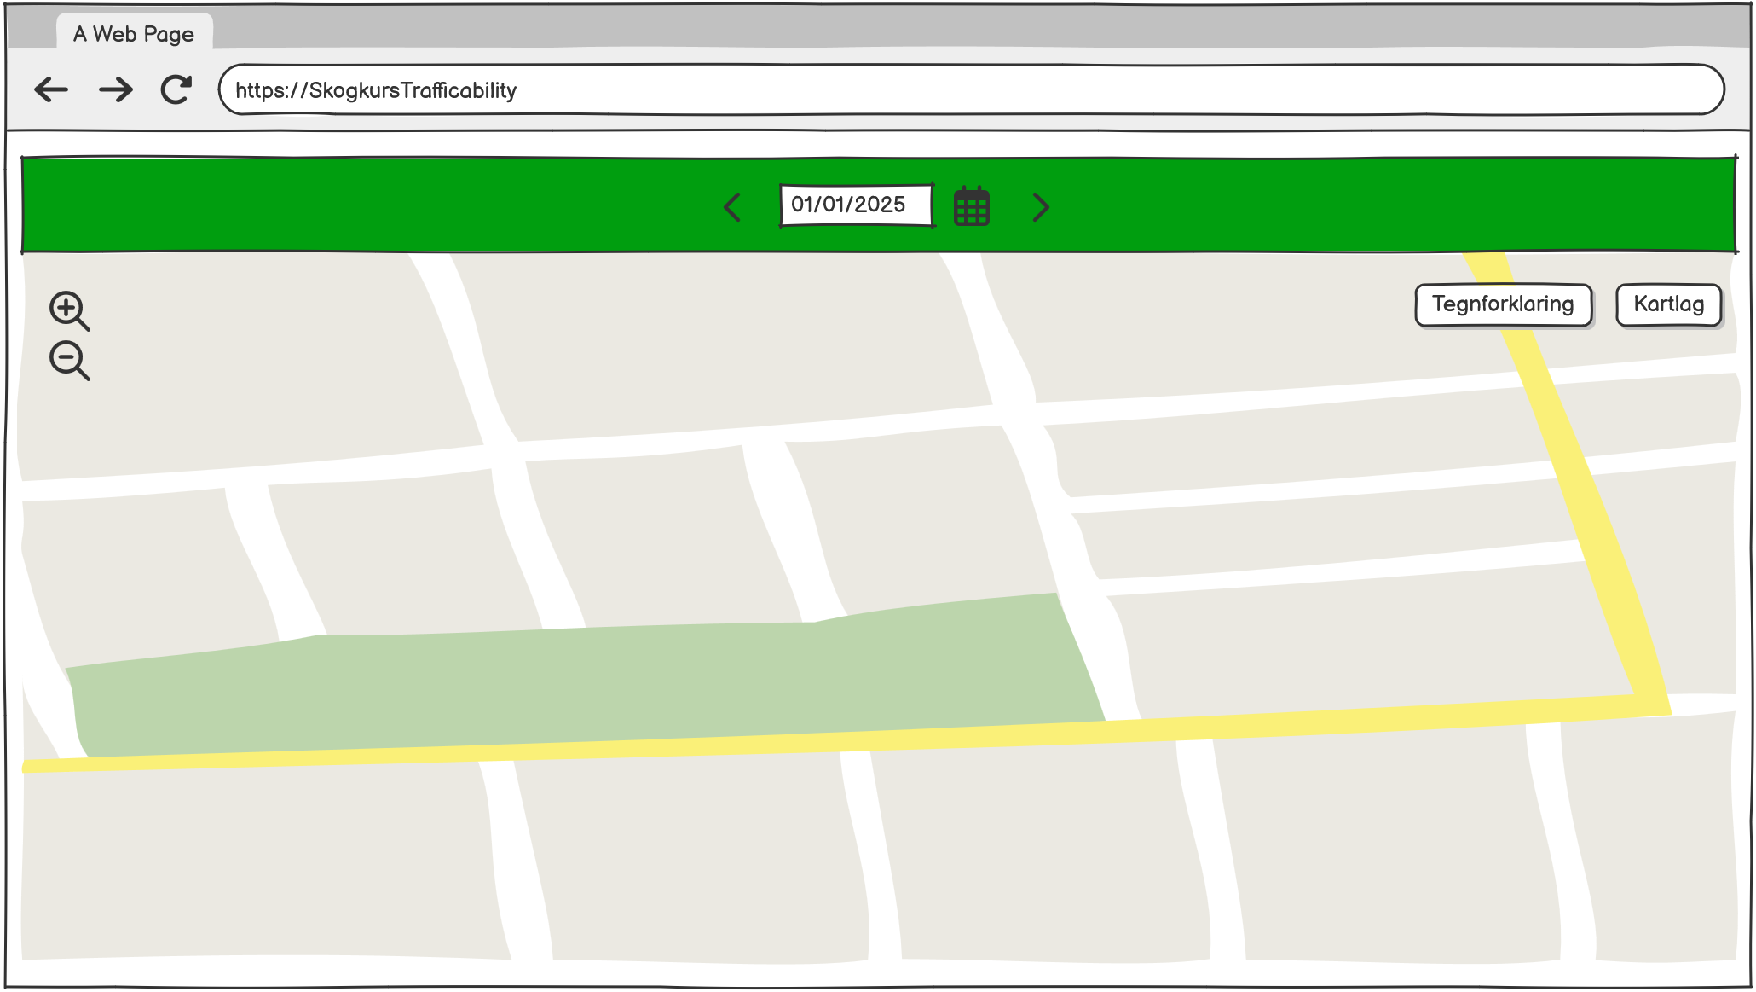
\includegraphics[width=\textwidth]{figures/wireframe_website_sidebars_closed.pdf}
         \caption{Sidebar closed}
         \label{fig:wireframe:closed}
     \end{subfigure}
     \hfill
     \begin{subfigure}[b]{0.45\textwidth}
         \centering
         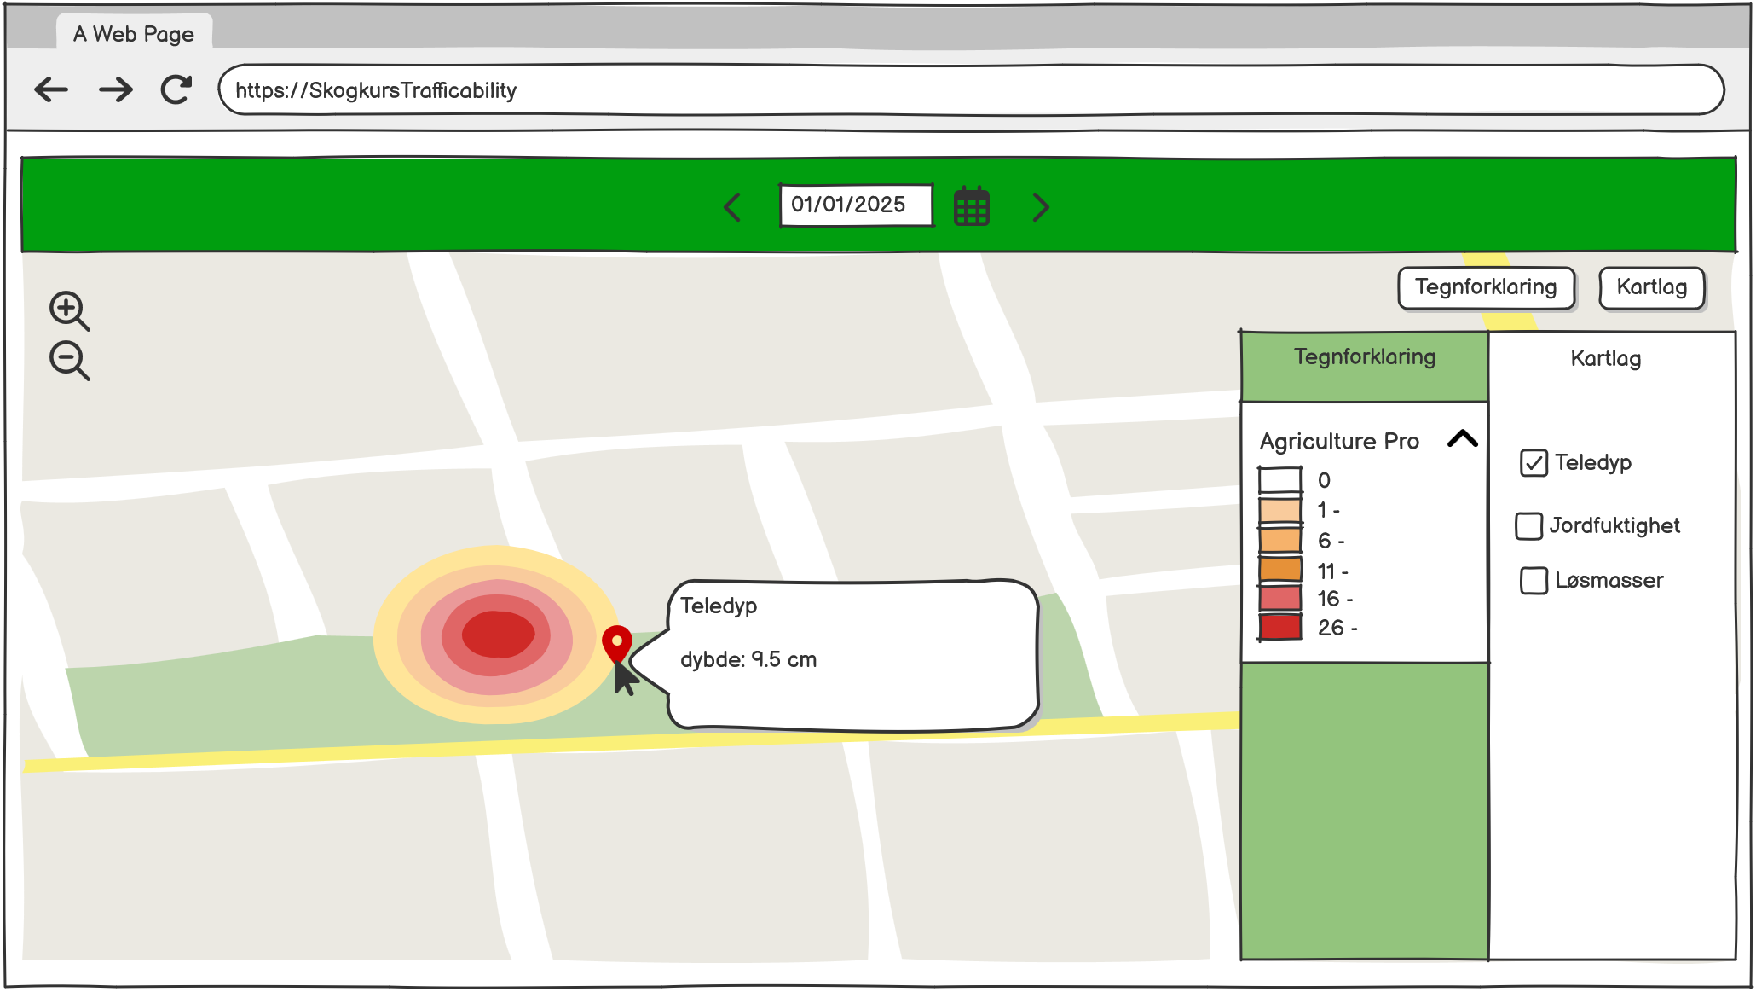
\includegraphics[width=\textwidth]{figures/wireframe_website_sidebars_opened.pdf}
         \caption{Sidebars opened}
         \label{fig:wireframe:opened}
     \end{subfigure}
    \caption{Wireframe of the website}
    \label{fig:wireframe}
\end{figure}

\subsubsection*{Early Iteration}

When we first began implementing the website using OpenLayers, we included several built-in components that seemed potentially useful. One of these was the overview map in the bottom-left corner, which provides a miniature version of the map view. This was helpful for orientation, especially when one or more map layers obscured the base map. We also added a scale line, a common feature in most map applications, to give users a sense of distance and scale.

In the version shown in \autoref{fig:website_layout_v1}, users could query all available map layers, such as the superficial deposit layer. While this functionality was helpful for debugging and comparing data across layers, it introduced unnecessary complexity into the \acrshort{ui}, especially from a user perspective. \textcolor{orange}{Repetering fra forrige section?}

A geolocation button was also included, allowing users to center the map on their current location if they consented to share it. However, when deploying the website on the backend server, we discovered that this feature only works over HTTPS due to browser security policies. Since the feature was not essential to the core functionality, and the project did not include setting up a valid HTTPS certificate, it was ultimately left non-functional in the deployed version.

\begin{figure}[h]
    \centering
    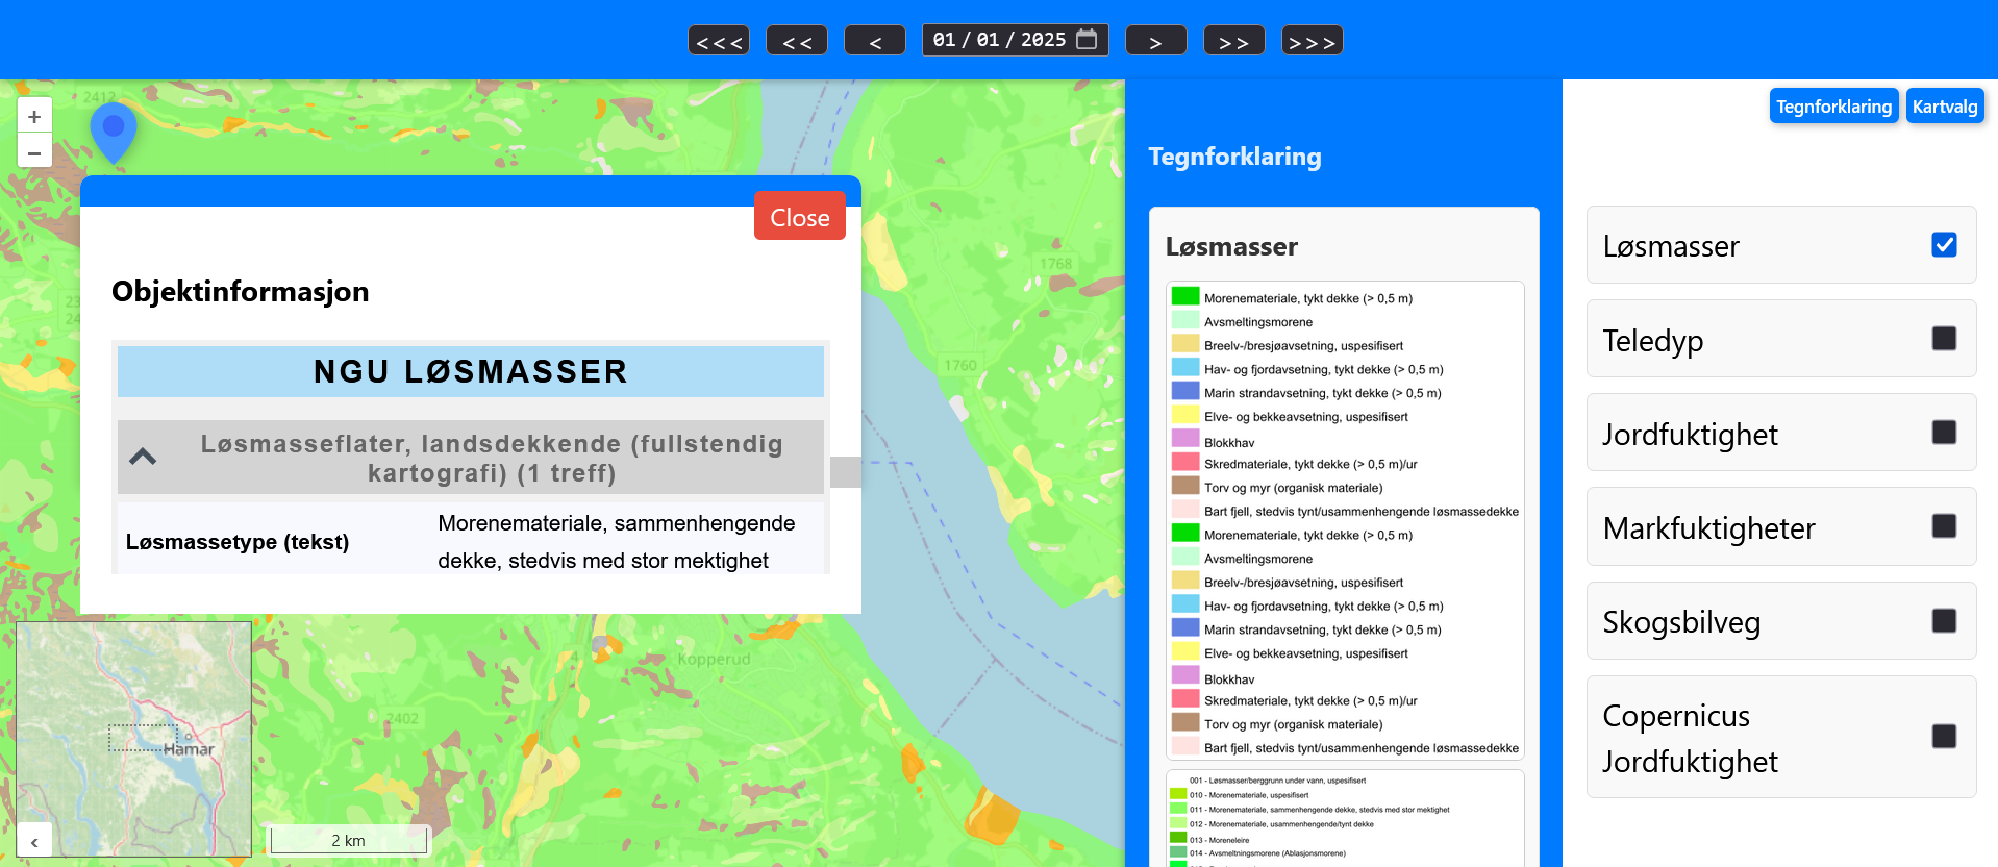
\includegraphics[width=1\linewidth]{figures/website_layout_v1.pdf}
    \caption{Early version of website}
    \label{fig:website_layout_v1}
\end{figure}

\subsubsection*{Final User Interface}

The final version of the \acrshort{ui} represents the \acrfull{mvp} and delivers the core functionality of the application.

As shown in \autoref{fig:website_layout_final}, several aesthetic and usability improvements were made. Icons were added to interface elements, such as chevron icons for the date picker at the top of the page, improving clarity and consistency. The base layer buttons in the bottom-left corner were updated with background images to visually indicate what each layer represents, making it easier for users to select the desired base map.

Based on feedback from the \gls{productowner}, a new feature was introduced to allow users to configure thresholds used to calculate the trafficability of forestry roads. This functionality was implemented in a new sidebar, following the same design as the existing sidebars for layer selection and legends. In this configuration sidebar, users can adjust parameters such as soil saturation and frost depth thresholds. As mentioned earlier, only the forestry road layer supports querying. This design choice simplified the user interface by focusing interactions on the most relevant layer. An example of the query result is shown in \autoref{fig:website_layout_final_sidebars}, where detailed information about a selected road segment is displayed.

To further improve usability, tooltips were added to interactive buttons, providing users with contextual hints about each element's purpose when hovered over.

The interface is primarily designed for desktop use, with layout and controls optimized for larger screens. While some functionality may be accessible on mobile devices, full responsiveness and mobile compatibility were not prioritized in this version.

\begin{figure}[h]
    \centering
    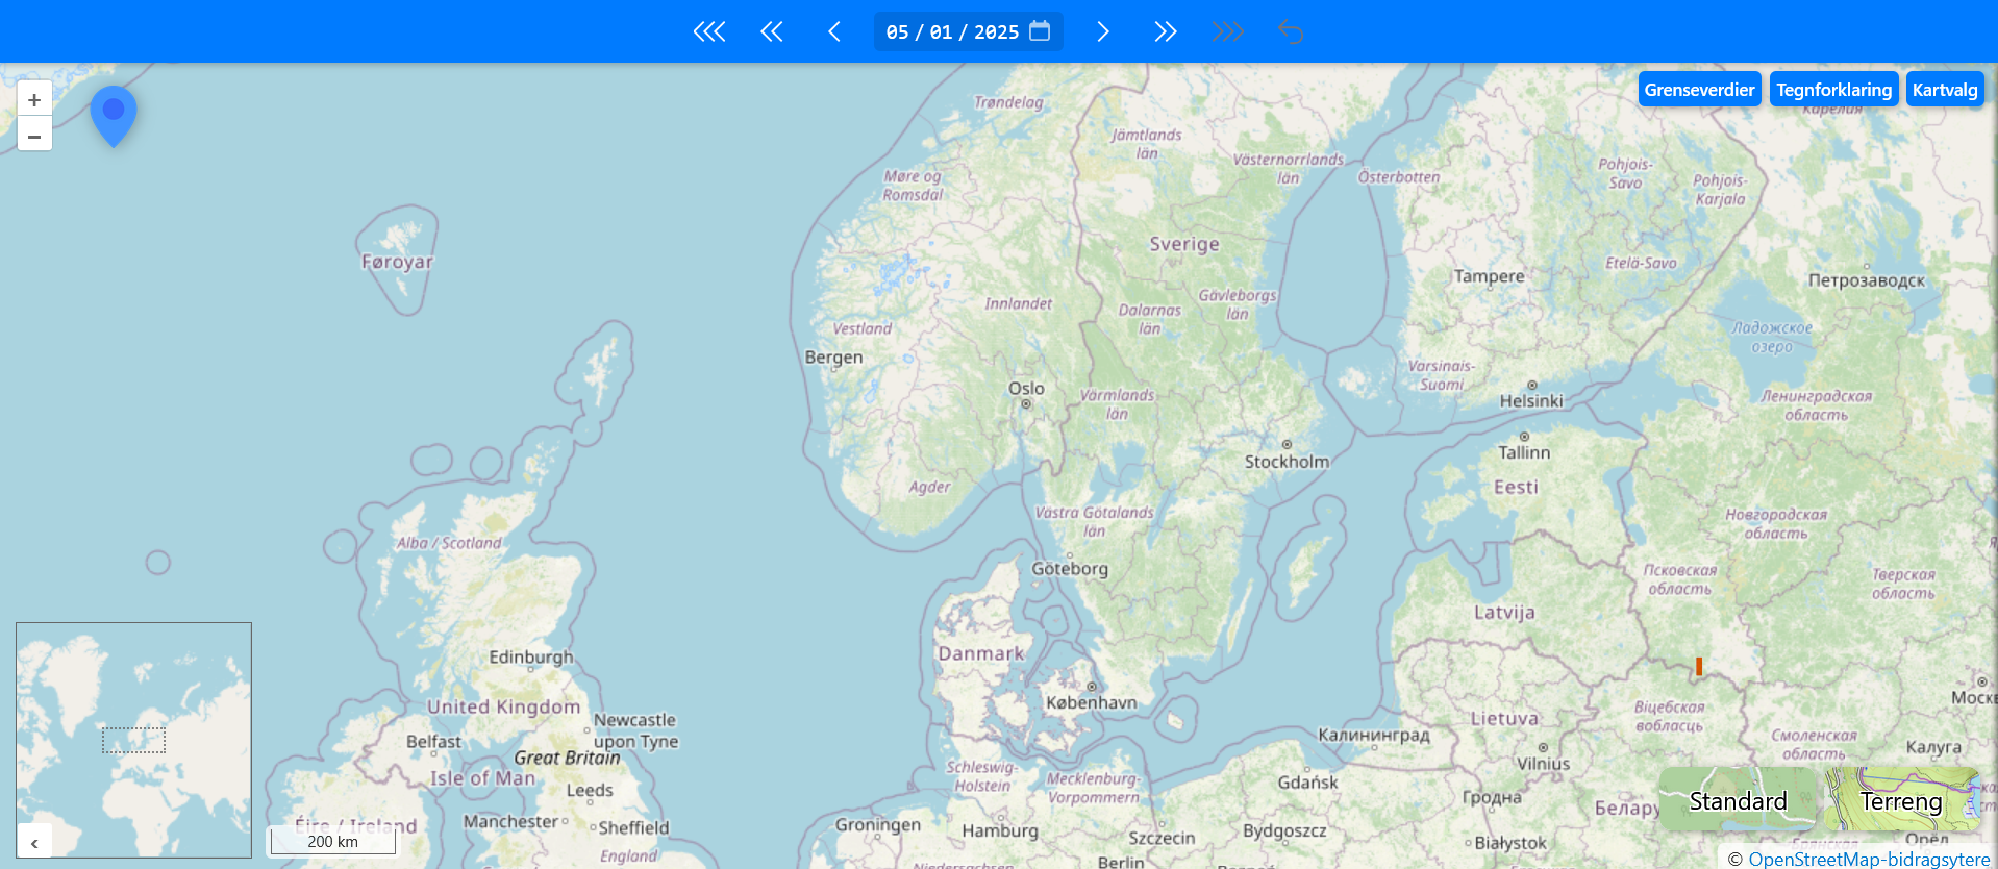
\includegraphics[width=1\linewidth]{figures/website_layout_final.pdf}
    \caption{Final version of website}
    \label{fig:website_layout_final}
\end{figure}

\begin{figure}[h]
    \centering
    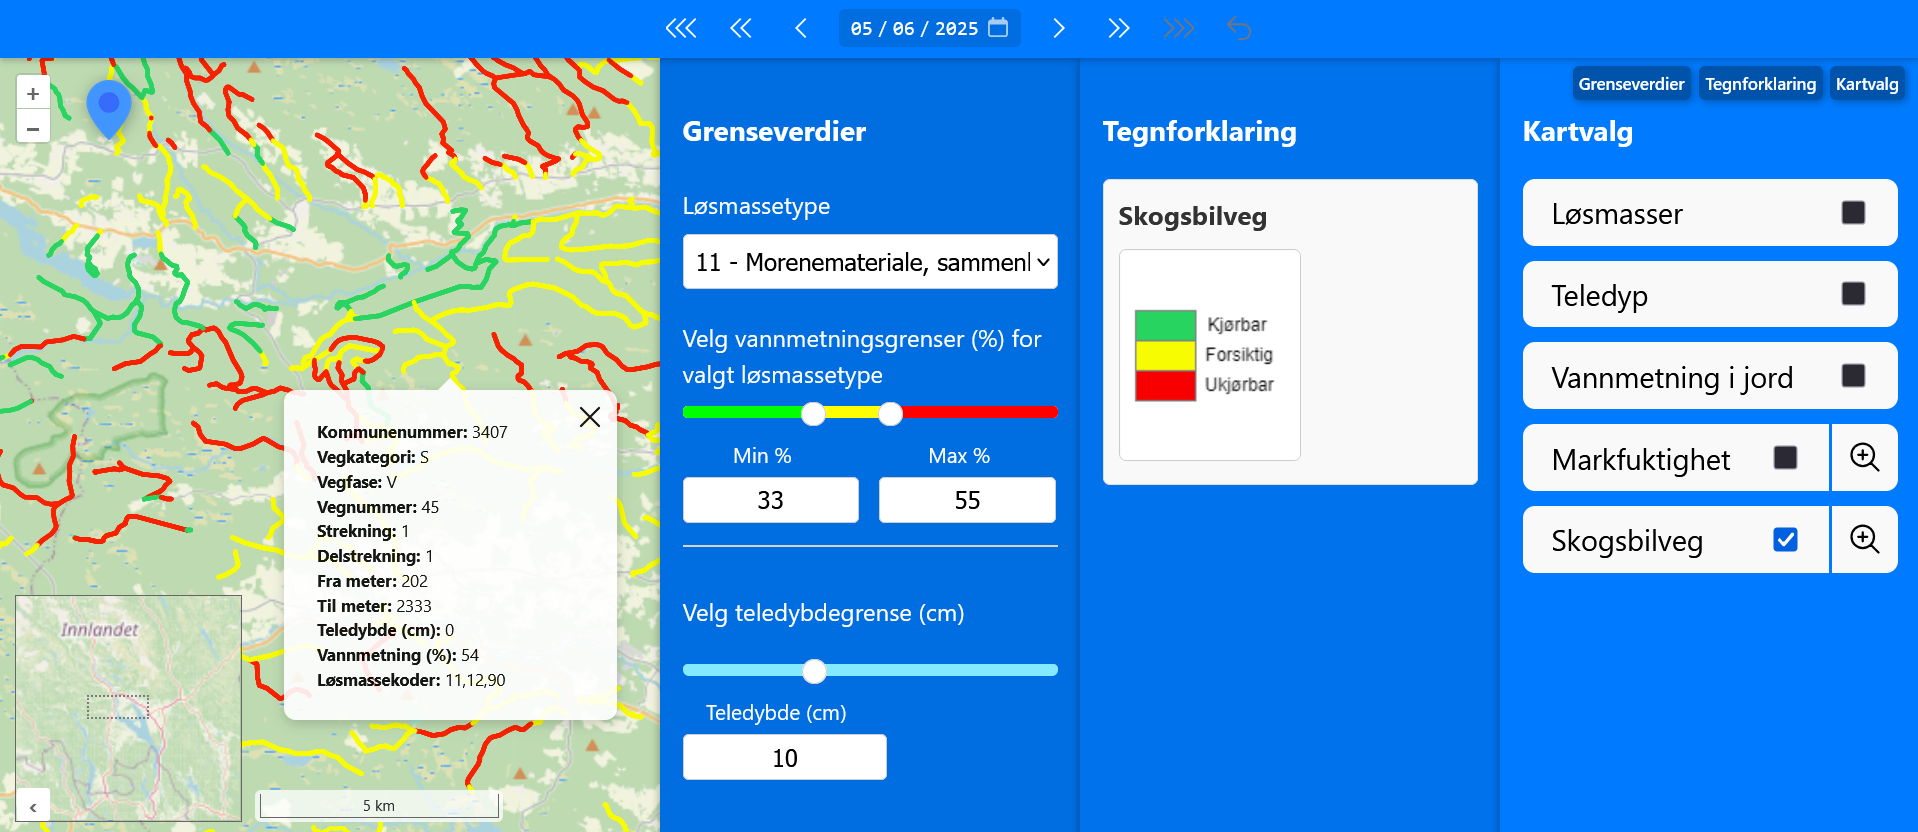
\includegraphics[width=1\linewidth]{figures/website_layout_final_sidebars.png}
    \caption{Final version of website with the sidebars opened}
    \label{fig:website_layout_final_sidebars}
\end{figure}


\subsection{Components}

As described earlier in \autoref{subsec:implementation:technologies:react}, the \acrshort{ui} is composed of multiple React components. While React allows for the reuse of pre-built components, in this application, all components were custom-built to suit specific requirements, except for a few controls provided by OpenLayers. React supports both class and function components, but for this project, we exclusively used function components. These are functions that receive props as input parameters from a parent component, and return TSX markup. Props are useful when a component requires data or functionality from its parent. TSX is a syntax extension similar to \acrshort{html}, but designed to be embedded within TypeScript functions \cite{react_component}.

\autoref{lst:react_component_example} shows an example of a React function component where the OpenLayers map instance is passed as a prop. This design makes it easy to integrate the component into the map, enabling communication between the component and the map. The component returns TSX markup, where the syntax distinguishes between standard HTML elements (e.g., \texttt{<div>}) and custom React components (e.g., \texttt{<ToggleLayers .../>}), the latter identified by their capitalized names. As shown in the example, components can also be nested within other components, allowing for a modular and hierarchical structure.

\begin{figure}[h]
\lstinputlisting[
    caption={Example of a React component},
    label={lst:react_component_example}
]{listings/component_example.tsx}
\end{figure}

When a user interacts with a component, it often needs to update in response. In React, this is handled using what is known as a component's state. Unlike regular variables, state values are preserved across re-renders. State can also be shared between components, a common and effective approach is to store the state in a parent component and pass it down to child components via props \cite{react_state}.

In \autoref{lst:react_state_example}, the \texttt{mapInstance} state is declared using the \texttt{useState} hook. This hook returns a pair: the current state value (\texttt{mapInstance}) and a function to update it (\texttt{setMapInstance}). In this example, an OpenLayers map instance is created and stored in the \texttt{mapInstance} state. This state can then be accessed and modified by other components that interact with the map by setting the state as their props.

\begin{figure}[h]
\lstinputlisting[
    caption={Example of a React state},
    label={lst:react_state_example}
]{listings/state_example.tsx}
\end{figure}

While state enables components to store and update values across renders, many interactive behaviors require performing actions as side effects. In React, such logic is handled using the \texttt{useEffect} hooks. This hook is a function that enables developers to run specific code after the component has rendered, and to react to changes in props, state, or other variables \cite{react_useEffect}.

A common use case for \texttt{useEffect} is to synchronize a component's state with external systems or APIs, in this case, synchronizing React state with the visibility of OpenLayers map layers. The effect shown in \autoref{lst:react_effect_example} monitors changes to the visibility state array and ensures that the corresponding OpenLayers layers are updated accordingly.

\begin{figure}[h]
\lstinputlisting[
    caption={Example of React \texttt{useEffect}},
    label={lst:react_effect_example}
]{listings/effect_example.tsx}
\end{figure}

\subsection{Date Picker}

An important feature requested by the \gls{productowner} was the ability to view forecasts of road trafficability. To support this, a date picker component was implemented, allowing the user to change the date for the data shown on the map.

The date picker consists of a standard \acrshort{html} date input element, along with buttons that increment or decrement the selected date by a day, a week, or a year. When the user selects a new date, all active map layers are re-queried and updated to reflect the data available for the new date. Only layers with available data for the selected date will be shown.

The dynamic data sources include historical data dating back to September 1, 1957, and forecast data extending nine days into the future. To prevent invalid selections, the date picker is restricted to this available date range.

\subsection{Map Integration with OpenLayers}

The interactive map component of the website was implemented using the OpenLayers library. The map was initialized within a custom React component, with its lifecycle managed using React hooks to ensure proper mounting and cleanup. The following types of layers were used:

\begin{itemize}
    \item \textbf{TileLayer}: Used for base map layers. It loads map images in small tiles, improving performance by enabling parallel loading and caching.
    \item \textbf{ImageLayer}: Used for dynamically changing map layers, such as those reflecting date-specific data. Unlike \texttt{TileLayer}, \texttt{ImageLayer} avoids inconsistencies caused by tiles loading at different times.
    \item \textbf{VectorLayer}: Used for client-side rendering of forestry roads from \gls{geojson} data. This layer type enables enhanced interactivity, styling, and feature manipulation.
\end{itemize}

\autoref{lst:wms_example} shows how an \texttt{ImageLayer} is implemented using a WMS source. To specify the WMS source we create a new \texttt{ImageWMS} object which holds values for the URL and the parameters (\texttt{params}). Together these make the full URL used to retrieve the images from the external WMS servers via the backend server.

The map layers are exported from their definition modules. This allows other React components to dynamically control aspects such as layer visibility or update parameters like changing the date of the map layer.

\begin{figure}[h]
\lstinputlisting[
    caption={Example of WMS implementation},
    label={lst:wms_example}
]{listings/openlayers_wms.tsx}
\end{figure}

\subsection{Trafficability Algorithm}\label{subsec:implementation:website:trafficability_algorithm}

As described earlier in \autoref{sec:technicaldesign:website}, the main feature of the website is to visualize forestry roads using a color-coded system: green, yellow, or red, to indicate their current trafficability.
These classifications are based on an algorithm that incorporates both meteorological and geological data.

Initially, we planned to perform these calculations on the backend to maintain cohesion and centralized control over the classification logic. By keeping all data processing on the server, we could ensure that the logic was consistent, easier to maintain, and independent of client-side variations. However, later in the project, the \gls{productowner} requested that users should be able to adjust threshold values for certain parameters dynamically using sliders. Since this would require recalculating the classifications in real time as the slider values changed, it became more efficient to move the algorithm to the frontend. This avoided repeated requests to the backend for each slider adjustment, as the map layer would only need to be fetched once and then re-styled dynamically on the client side.

As shown in \autoref{lst:forestryroads_styling}, each feature rendered on the map includes \gls{geojson} properties for relevant meteorological and geological data, specifically, frost depth, soil saturation, and superficial deposit type. These values are compared against the threshold values selected by the user to determine the color used for each road segment.

The function that determines the color of the road is shown in \autoref{lst:trafficability_algorithm}. If the frost depth exceeds the threshold, the road is classified as having good trafficability (green). If not, the soil saturation value is used to determine whether the trafficability is moderate (yellow) or poor (red), based on user-defined minimum and maximum thresholds.

\begin{figure}[h]
\lstinputlisting[
    caption={Styling of forestry roads},
    label={lst:forestryroads_styling}
]{listings/forestryroads_styling.ts}
\end{figure}

\begin{figure}[h]
\lstinputlisting[
    caption={The trafficability algorithm},
    label={lst:trafficability_algorithm}
]{listings/trafficability_algorithm.ts}
\end{figure}

\subsection{Integration with Backend}

All map data displayed on the website is fetched through the backend server. Each map layer is implemented using an OpenLayers object that sends requests to a specified URL. The response format depends on the type of map layer.

As shown in \autoref{lst:url_example}, \texttt{TileLayer} and \texttt{ImageLayer} use either an XYZ tile URL or a \gls{wms} URL, both of which return rendered map images. In contrast, \texttt{VectorLayer} uses a \gls{wfs} URL to request raw vector features, which is returned in the \gls{geojson} format.

\begin{figure}[h]
\lstinputlisting[
    caption={Example of OpenLayers URL configurations},
    label={lst:url_example}
]{listings/openlayers_url_examples.tex}
\end{figure}

To improve performance and reduce unnecessary network traffic, layers are loaded dynamically based on the user's interaction with the map, such as panning or zooming. Certain layers are only activated at specific zoom levels or within a defined spatial extent to ensure efficient resource usage.

\section{Server}\label{sec:implementation:server}

This section describes the implementation of the server, which serves as the source of information for the website. Additionally, key functionality and iterations will be outlined. The backend server consists of two main parts: a proxy for \Gls{wms} services and an endpoint for the forestry road algorithm. 

\subsection{Forestry Road Algorithm}\label{subsec:server:forestroadalgorithm}

\textcolor{orange}{
Hva det er (api, (REST?)) \\
Hvordan den funker (Hente veidata, cluster, query, send tilbake) \\
Hvorfor vi gjorde det slikt (kanskje ikke? \\
Skrive at vi gikk ut ifra at veiene er lagd av løsmassene i området. Kanskje skrive om de andre... 
) \\
FJORDKATALOG
}

... An overview of the external libraries used is shown in \autoref{tab:golibraries}. ...

\begin{table}[h]
    \centering
    \begin{tabular}{|l|l|}
        \hline
        \textbf{Library} & \textbf{Description} \\
        \hline
        joho/godotenv & Loads environment variables from .env files. \\
        rs/zerolog & Zero Allocation Logger. \\
        tidwall/rtree & R-tree implementation for spatial querying. \\
        twpayne/go-geom & Efficient geometry types for geospatial applications. \\
        twpayne/go-shapefile & Native Go reader for ESRI Shapefiles \\
        \hline
    \end{tabular}
    \caption{Overview of used Go libraries}
    \label{tab:golibraries}
\end{table}

\subsection{Proxy}\label{subsec:server:proxy}

As described in \autoref{sec:systemarchitecture}, we wanted a clean architecture where all requests are routed through the backend server. The implementation of this idea is the proxy endpoint on the server. Proxies are loaded from a JSON\footnote{\url{https://www.json.org/}} file, where each key denotes a specific proxy endpoint, and the corresponding value specifies the target URL to which requests should be forwarded. \autoref{lst:proxycreation} shows how the proxy endpoints are loaded, in addition to the creation of two endpoints for routing the base map layer requests. 

\begin{figure}[h]
\lstinputlisting[
    caption={Creation of proxy endpoint},
    label=lst:proxycreation
]{listings/proxycreation.go}
\end{figure}

\subsection{Optimization}\label{subsec:server:optimization}

Early iterations of the forest road retrieval and processing algorithm were computationally expensive, resulting in long response times when querying the forest road layer.

\subsubsection{SeNorge}\label{subsubsec:implementation:optimization:senorge}

The backend would initially query the SeNorge API once for every road, which would quickly overload the API server leading to long processing times. Additionally, the SeNorge API would not accept multiple coordinates within each grid-cell. SeNorge uses a grid system to divide Norway into \qty{1}{\kilo\meter\squared} cells, and calculate all their climate projections as an average within each cell \cite{senorge_watermap}. 

Lacking documentation of how the grid-cells were initially declared, in addition to a deprecated service for transforming coordinates to cell indexes, prompted further investigation into the SeNorge grid-cells. Findings showed that each grid-cell had borders that lined up with the UTM zone 33N projection system, where the latitude and longitude of each grid intersection were a multiple of \qty{1000}{}. In other words, each grid is centered on a UTM coordinate that is a multiple of $\qty{1000}{}\pm\qty{500}{}$.

The findings made it possible to cluster the forest roads into their closest SeNorge grid-cell, without explicitly knowing which grid-cell was closest. The coordinate of the cluster center could then be used to send a singular request to the SeNorge API, drastically increasing the amount of roads that could be processed at once. Listing \ref{lst:clusterforestroads} shows the implementation of the clustering, where the forest roads are clustered into a sharded map for fast concurrent read and writes.

\begin{figure}[h]
\lstinputlisting[
    caption={Clustering of forest roads},
    label=lst:clusterforestroads
]{listings/clusterwfsresponsetoshardedmap.go}
\end{figure}

\subsubsection{Spatial querying}

Another large optimization was made related to how superficial deposit along the roads were queried. Initially, the middle of each road would be used to query NGU's \Gls{wms} server\footnote{\url{https://geo.ngu.no/kart/losmasse_mobil/}}, leading to a large amount of HTTP requests. These HTTP requests would then quickly overload the \Gls{wms} server, leading to extensive response times.

This was solved by downloading the superficial deposit data and reconstructing it into a map in-memory. The data was downloaded from GeoNorge\footnote{\url{https://kartkatalog.geonorge.no/}} and is available under the NLOD license\footnote{\url{https://data.norge.no/nlod/no/2.0}}. The reconstruction of the spatial data can be found in \autoref{lst:spatialindex}, where each record is read and reconstructed into an R-tree. An R-tree allows for effective querying of spatial data by grouping nearby objects and represent them with their bounding box in the next higher level of the tree \cite{rtreewikipedia}. Having the spatial data in-memory allowed for a greater number of queries along the road.

\begin{figure}[h]
\lstinputlisting[
    caption={Building of spatial index},
    label=lst:spatialindex
]{listings/readshapefileandbuildindex.go}
\end{figure}

\subsubsection{Goroutines}

As previously stated in \autoref{subsec:implementation:technologies:go}, Go was chosen partly due to its native concurrency functionality. This proved to be a wise decision, as Goroutines was a large part of reducing the processing times. The amount of features (forestry roads) shown on the map at once can range from zero to several thousands, depending on the zoom level used. Processing these sequentially would lead to extensive processing times, whereas use of parallel processing ensured consistently low loading times, even when handling large volumes of data. An example of how Goroutines was used can be seen in \autoref{lst:clusterforestroads}, where a wait-group and a semaphore are used to synchronize and limit the amount of Goroutines used.

\begin{comment}
UTFORDRINGER OM IMPLEMENTASJON HER:
    - Kilder
        - Senorge dårlig dokumentasjon til API
            - Bruker annen endpoint istedenfor
    - Finne gode og nøyaktige data
    - Gjøre om data til WMS/noe vi kan vise
    - Gjøre om WMS/kartdata til rød, grønn eller gule veier
    - Konvertering av koordinater, f.eks. fra epsg:3857 til epsg:25833
    - Klassifisering av skogsbilveger
        - Hente teledyp data for flere veger (WMS vs. REST API)
        - Teletyp var vanskeligere enn forventet siden API-en brukte et dårlig dokumentert grid-system.
\end{comment}

\chapter{Deployment}\label{chap:deployment}

This chapter describes how the application is deployed using Docker and Docker Compose on NTNU's SkyHiGh platform. It covers the technical setup, including how Docker images are built with GitHub Actions and published to the GitHub Container Registry. The chapter also outlines what would be required for Skogkurs to deploy the system on their own infrastructure.

\section{SkyHiGh}

Throughout the latter half of the project, the application was deployed with Docker Compose on NTNU's shared cloud computing platform, SkyHiGh\footnote{\url{https://www.ntnu.no/wiki/display/skyhigh}}. SkyHiGh is IIK's installation of OpenStack\footnote{\url{https://www.openstack.org/}}, located in Gjøvik. SkyHiGh allows users to get access to either a single virtual machine with an operating system of their choice, or project where they are able to create networks, routers and virtual machines at their own will.

The usage of SkyHiGh in the project primarly included four virtual machines. As described in \autoref{chap:developmentprocess}, we used two virtual machines for a backup server and the time tracking server. Two virtual machines was used to deploy the application, one for hosting the superficial deposit and fjord data, and one for running the application itself. A dedicated server for hosting superficial and fjord data was needed due to the large size of the files would not allow them be kept on GitHub. The usage of this virtual machine will be detailed in the coming sections. The virtual machine
% Hvordan vi har deploya: SkyHiGh -> Ubuntu VM -> tmux -> Docker Compose
%which is ran inside tmux\footnote{tmux is a terminal multiplexer. It lets you switch easily between several programs in one terminal, detach them (they keep running in the background) and reattach them to a different terminal.} on a virtual machine on SkyHiGh.

%The application VM was configured with Docker Compose and hosted on a virtual Ubuntu machine. To keep the application running continuously, it was executed inside a tmux\footnote{\url{https://github.com/tmux/tmux/wiki}} session, a terminal multiplexer that allows persistent and detachable command-line sessions. This setup proved sufficient for our development and demonstration purposes, given the low uptime and scalability requirements.

This approach was chosen due to its simplicity and the low availability requirements. Docker Compose require less configuration compared to other solutions like Kubernetes\footnote{\url{https://kubernetes.io/}} and Docker Swarm\footnote{\url{https://docs.docker.com/engine/swarm/}}, which makes it easy to use and ideal for small-scale deployments. However, this simplicity comes at the cost of limited scalability and orchestration features, making it less suitable for complex, production-grade environments. This will be further discussed later in \autoref{chap:discussion}.

\section{Docker and Docker Compose}
%Explain the basics of Docker and Docker Compose.
%Detail how containers are networked, how environment variables and volumes are configured.
%Mention the docker-compose.yml structure (briefly, or refer to an appendix/code repo).
%All Docker containers are made using a Docker image \cite{dockerwikipedia}.

As previously described in \autoref{subsec:implementation:technologies:docker}, Docker Compose is used for defining and running multi-container applications. Compose also provides configuration options like defining environment variables, mapping ports and defining networks containing containers. The application consists of two containers on the same network: website and server. These two containers are deployed on the same network with Docker Compose.


\section{GitHub Actions}
%Introduce GitHub Actions as a CI/CD tool.
%Include a brief sidebar or paragraph explaining CI/CD if your audience may not know it.
%Describe how each commit to specific branches triggers the build process.
%Explain that images are pushed to the GitHub Container Registry automatically.
%Reference where Dockerfiles and workflows are found in the repository.

The Docker images used to build the application are made using GitHub Actions\footnote{\url{https://github.com/features/actions}}. 
HVA ER ACTIONS? (CICD PIPELINE)
-->
Any commit pushed to the server or website repositories will trigger the action, which then builds the image and pushes it to GitHub Container Registry\footnote{\url{https://docs.github.com/en/packages/working-with-a-github-packages-registry/working-with-the-container-registry}}. All Docker images are built using a text document that contains all the commands a user could call on the command line to assemble an image, called a Dockerfile \cite{dockerfiledocs}. The Dockerfiles along with the GitHub Action for the website and server can be found in their respective repositories (see \autoref{tab:githubrepositories}).

\section{Building the Containers}

\subsection{Website Container}
%Built using Vite, a modern frontend build tool.
%Explain the vite build process that compiles the static assets.
%Describe how the output is served in production (e.g., using a static file server or Node.js).
%Optionally include: why Vite was chosen over alternatives like Webpack.


% Kanskje ikke ha med det under:
%Vite is a modern build tool optimized for frontend development. It offers a fast development server, which is currently used to run the website during development. Ideally, Vite would only be used to build the application for production, with a separate tool or server handling deployment \cite{vite}.
%Running the development server manually requires Vite, Node.js, and npm to be installed. From the project's root directory, the server can be started with the command: \texttt{npm run dev}. However, since Docker is used to containerize the application, running this command manually is unnecessary.

\subsection{Server Container}
%Built using the Go toolchain.
%Mention that the server binary is compiled with go build.
%Describe the Dockerfile setup for Go, such as using a multi-stage build (if applicable).
%Highlight efficiency in build times, static binaries, etc.



\section{Deployment by Skogkurs}
%Provide clear steps required for external deployment:
%Downloading necessary datasets.
%Preprocessing data using provided Python script.
%Handling of secrets and environment variables.
%Options for building and deploying images (CI/CD vs. local).
%Updating the Docker Compose config.
%Consider including a checklist-style table or bullet list to make this actionable.

Several steps are required for Skogkurs to deploy the application on their own servers. First, the superficial deposit and fjord datasets must be downloaded from Kartkatalogen\footnote{\url{https://kartkatalog.geonorge.no/}}. Additionally, the fjord dataset must be preprocessed with a python file that is provided in the server repository. If Skogkurs intends to replicate the original approach to building the Docker images, datasets must be made accessible via SSH, and the relevant environment and secret variables must be configured within the CI/CD pipelines. Alternatively, the Docker images can be built locally before being pushing to a registry. In either case, the Docker Compose configuration must to be updated the new image ownership.

\chapter{Testing and User Feedback}

\textcolor{orange}{NOE TEKST}

\section{User Testing}

\textcolor{orange}{NOE TEKST}

\subsection{Result}

\textcolor{orange}{NOE TEKST}

\subsection{Product Iteration and Polish}

\textcolor{orange}{NOE TEKST}

\chapter{Discussion}\label{chap:discussion}

This chapter presents a reflection on both the development process and the final product. It examines how the project evolved in relation to the original goals, highlighting what worked well, what could have been improved, and the challenges encountered along the way. The chapter discusses the choice of technologies, project management practices, and team collaboration. It also evaluates the effectiveness and limitations of the final solution, comparing it with existing alternatives and identifying unexpected findings. Broader considerations, such as sustainability and the role of AI in the project, are explored. Finally, the chapter outlines potential directions for future work and improvements to both the product and the project approach.

\section{Process}\label{sec:discussion:process}

This section provides a reflection on the project's development process, covering both planning and execution. It examines how the initial project plan guided the work, the technologies that were selected, and the software development methodology that was followed. The section also evaluates the collaboration within the group, including how communication was handled and how responsibilities were distributed. In addition, it highlights areas where the process could have been improved, and describes how AI tools were used throughout the project to support development, planning, or writing tasks.

\subsection{Project Plan}\label{subsec:discussion:process:projectplan}

Looking back, we were able to mostly follow the project plan, but there were certain tasks that either were rescheduled or removed entirely for practical reasons. The most difficult part of planning was knowing how much time to allocate to each part of the project. There were multiple times where we had either worked faster than expected or had to postpone tasks due to unforeseen issues. Using tools like Planning Poker could have made this easier. The goal of the method is to make estimations individually without being influenced by the other group members \cite{planningpokerwiki}. Additionally, our time estimations were based on high-level task descriptions, which proved too abstract. Breaking tasks down into more granular, concrete sub-tasks could have led to more accurate and realistic estimates.

One of the biggest strengths of the project plan was the structure provided by Scrum and the use of sprints. The plan's division into eight sprints allowed us to stay focused and iterative, and it gave us frequent opportunities to re-evaluate priorities and progress. However, we found that the sprint content sometimes had to be adjusted mid-way through to accommodate emerging challenges, such as unexpected bugs, changes between data sources, or new feature requests from the Product Owner. Knowing this, the sprint length could potentially have been shorter, e.g., the first few sprints were 1-week then the later ones could have been 2-weeks. 

Our Gantt chart helped define clear milestones, like the MVP, and these helped us stay aligned with deliverables. Nevertheless, actual progress often did not align perfectly with the chart. For instance, early on we had a whole sprint for research, data collection and system design. In hindsight we only needed half a sprint for this and therefore we started designing the website which was planned for the next sprint. In later sprints we had planned user tests which kept getting pushed back, and in the end the formal user tests were replaced with feedback from the Product Owner and a presentation of the product for potential stakeholders.

The inclusion of the vacation in the plan was helpful, and having accountability measures, like compensating for delays by using it as a buffer, proved valuable in practice. The group contract and routine rules also helped maintain consistent effort and communication.

Another challenge we faced was scope control. As anticipated in the risk analysis (see \autoref{appendix:project_plan}), there was some pressure to expand the scope by including additional features or data sources. For example, the Product Owner emphasized that the product should at least function reliably in the local area (Gjøvik), but the final version ended up supporting the entire country. While this broader scope added value, it also introduced complexity and potential performance issues. Regular sprint meetings with our supervisor were essential in helping us manage these demands, keeping the project aligned with its core goals and preventing uncontrolled feature creep.

\subsection{Technologies}

This section contains a reflection of the different technologies and tools used throughout the project. We discuss both the client-side and server-side components, as well as supporting tools that contributed to collaboration, version control, and project management. The chosen technologies were selected based on factors such as ease of integration, documentation quality, performance, and our team's familiarity with them, or lack thereof.

\subsubsection{Website}

The chosen technologies for the website, TypeScript, React, and OpenLayers, proved to be well-suited for the project. Although we had little prior experience with these tools, their extensive documentation allowed us to quickly learn them throughout the development process.

While the overall scope of the application is moderate, using TypeScript instead of JavaScript improved type safety and reduced the likelihood of runtime errors. This added confidence during development and helped maintain code quality.

We had limited prior experience with web development, so we cannot directly compare React to building a website without a similar library. However, React's component-based structure made it easy to build and reuse interface elements, which likely made the development process more efficient and maintainable.

When selecting a map library, we evaluated several options, including more widely used ones like Leaflet and Mapbox. While these libraries are known for their ease of use and strong community support, we ultimately chose OpenLayers due to its built-in GIS functionality and flexibility. Unlike MapBox, OpenLayers is fully open-source and free to use, without licensing restrictions. In hindsight, while OpenLayers has a steeper learning curve, its comprehensive feature set allowed us to implement advanced functionality, such as WMS layers and raster overlays, without relying on third-party plugins, as would have been necessary with Leaflet.

\subsubsection{Server}

As described in \autoref{chap:implementation}, we made good use of the advantages of Go. Our prior experience with Go allowed us to implement advanced optimization techniques like multi threading and clustering. Consequently, the time spent developing the server was shorter compared to the website, as less time was used reading documentation and exploring unfamiliar frameworks.

Go's extensive package registry\footnote{\url{https://pkg.go.dev/}} of open-source libraries were vital for implementing certain functionality. Without the packages go-shapefile and go-geom, the superficial data could not have been stored locally and would have to have been sourced from an \acrshort{api}. This would lead to extensive processing times, as we query every \qty{10}{\meter} of road, and an external \acrshort{api} is considerably slower than in-memory data.

\subsubsection{Other Technologies}

\textcolor{orange}{traggo, docker, skyhigh etc.}

The use of GitHub for both version control and task management via the Kanban board\footnote{\url{https://github.com/orgs/skogkursbachelor/projects/1}} made it easy to track progress and adjust tasks as needed. This complemented the Scrum framework well and allowed us to keep the project transparent and adaptable. Storing everything in GitHub within its own repository proved to be very useful, as it allowed us to keep all project files in one centralized location. By backing up all documentation and diagrams, we ensured that nothing would be lost and provided easy access for all group members. Additionally, we decided to separate the frontend and backend into distinct repositories. This approach enhanced maintainability, since the frontend and backend are written in different programming languages and are deployed differently.

Using Traggo for time tracking made it straightforward to categorize work using tags. As a self-hosted and free solution, it did not require creating additional user accounts, which made access simple and efficient. It included all the core features we needed, though it lacked some useful extras, such as the ability to filter by multiple tags at once. For example, it was not possible to easily see how much time a specific user spent on a particular task.

\subsection{SDLC Model / SCRUM}

\textcolor{orange}{NOE TEKST}

\subsection{Communication}

The communication between the group members was consistently productive throughout the project. Knowing each other personally prior to the project allowed us to be blunt and precise during discussions, keeping the collaboration efficient, calm, and productive.

\gls{productowner} and our supervisor ...

\subsection{Work Allocation}

\textcolor{orange}{blabla}

\autoref{tab:timetrackedbymember} shows the total time of work for each month by the two members.

\begin{table}[h]
    \centering
    \begin{tabular}{c|c|c|c}
        \hline
        \textbf{Month} & \textbf{Bjørnsen} & \textbf{Houmb} & \textbf{Total} \\
        \hline
        January  & 61h 39m  & 62h 58m  & 124h 37m \\
        February & 80h 6m   & 79h 17m  & 159h 24m \\
        March    & 88h 4m   & 88h 20m  & 176h 24m \\
        April    & 99h 40m  & 102h 38m  & 202h 18m \\
        May      &        &        &        \\
        \hline
        Total & & & \\
        \hline
    \end{tabular}
    \caption{Tracked time by month and group member}
    \label{tab:timetrackedbymember}
\end{table}

% Skriv mer om time fordeling, f.eks. hvorfor mer timer i mars enn januar etc.

\autoref{fig:time_tracking_by_type} shows the total time of work for each month by the two members.

% KANSKJE IKKE TA SKJERMBILDE, LAG HELLER CHART MED LATEX f.eks. (pfg-pie).
% tar screen på mac for bra oppløsning
\begin{figure}[h]
    \centering
    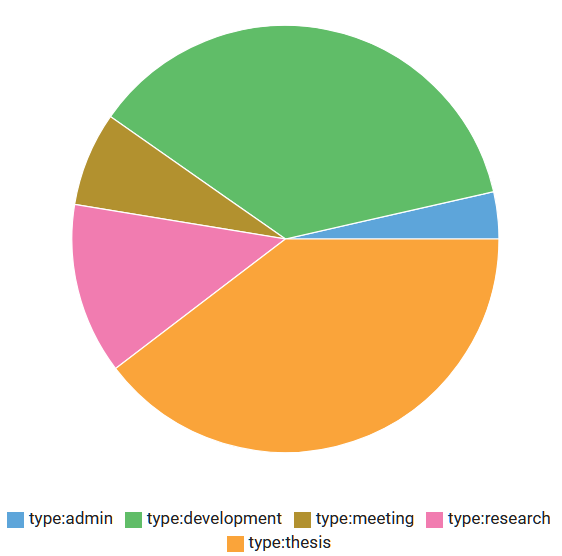
\includegraphics[width=0.5\linewidth]{figures/traggo_pie_chart_by_type.png}
    \caption{Pie chart of time spent in total per work type}
    \label{fig:time_tracking_by_type}
\end{figure}

\textcolor{orange}{OPPDATER PIECHART OG TABLL FØR LEVERING}

% SKRIV OM TIDSFORDELING FOR DE FORSKJELLIGE OPPGAVENE (THESIS, DEV, osv.)

\subsection{Improvements}

\textcolor{orange}{Hvordan forbedre tidsestimering? mangel på formell brukertesting? }

\subsection{Use of AI}

\textcolor{orange}{NOE TEKST}

\subsubsection{Learning}

\subsubsection{Inspiration}

\subsubsection{Spellcheck}



\section{Product}

\subsection{Goal Assessment}

\textcolor{orange}{blabla revisit the goals from \autoref{chap:requirements}}

\subsubsection{Product Goals}

The primary goal of the project was to develop and test a \textbf{prototype system for fully digital modeling of forestry road load-bearing capacity under varying conditions throughout the year.} 

\\ \textcolor{orange}{Siden det ikke var satte krav for produktet annet en det over, valgte vi å definere tasks selv som ville gi en pekepin på hva vi har oppnådd med sluttproduktet: marked in \textbf{bold}}


\textbf{Decide and gather relevant geological and meteorological data, which may include superficial deposits, soil moisture, ground water, and ground frost} 

The product integrates various geological and meteorological data sources, as described in \autoref{chap:mapdatasources}. Historical, real-time and forecast values for frost and soil moisture are available alongside superficial deposit data.

\textbf{Identify and implement suitable data sources and APIs for continuous updates.} 

As described in \autoref{chap:implementation}, data is sourced from various providers which required different approaches to incorporate in the application.

\textbf{Develop a rule-based model to classify road conditions based on environmental factors.}

\textbf{Extend the model to provide a forecast of road conditions at least a week in advance.}

\textbf{Design and develop an interactive map-based website for intuitive accessibility.}

\textbf{Implement a GIS-based visualization with real-time updates and historical road condition tracking.}

\textbf{Ensure that the system is optimized for transport managers, with a user-friendly interface that allows efficient decision-making.}

\textbf{Evaluate the accuracy and usability of the system by testing with real-world data.}

\textbf{Conduct user testing with transport managers or forestry stakeholders to assess the effectiveness of the interactive interface and forecasting capabilities.}

\textbf{Incorporate potential user feedback.}


According to the feedback we received from stakeholders, the product was intuitive and easy to use. The traffic-light system used to display road trafficability was especially well-received, as it provided a clear and familiar visual language. While the overall feedback was positive, some usability improvements were suggested. For example, although users could adjust the threshold values used in road classification, they wanted the ability to customize these values for specific roads or locations. Additionally, these thresholds should persist between sessions to avoid repetitive configuration.

\subsubsection{Impact Goals}

The project aimed to deliver real-world value by improving decision-making processes related to forestry road usage. The following impact goals outline the intended benefits for end-users and stakeholders:

\begin{itemize}
    \item Reduced uncertainty for transport managers when setting the routes using forest roads.
    \item To validate the prototype's feasibility and effectiveness by conducting tests with end-users, such as transport managers, to assess its performance and usability in real-world scenarios.
\end{itemize}

\subsubsection{Learning Goals}

In addition to delivering a functional prototype, the project served as a valuable learning experience. The goals below reflect the desired technical and professional growth for the project participants:

\begin{itemize}
    \item Gaining insight in implementing interactive maps and geospatial data on web pages.
    \item Leveraging RESTful APIs for efficient data integration.
    \item Acquiring hands-on experience collaborating with real-world companies and products.
    \item Gaining experience working in a team environment, improving collaboration and communication skills.
    \item Conducting user tests and implementing feedback. XXX
    \item Developing a deeper understanding of the software development life cycle while actively practicing agile methodologies, like Scrum and Kanban.
    \item Enhancing application performance by implementing concurrency and optimizing parallel processing.
    \item Expanding proficiency in containerization techniques, particularly through hands-on experience with Docker.
\end{itemize}

\subsection{Limitations}

% Feilkilder (kartdata) e.g. https://www.senorge.no/WaterMap
% Vanskelig å få tilgang til satellittdata fra SMAP & SENTINENTAL-1. For å få prognose må man ha en modell for å regne ut.

\textcolor{orange}{- Bad performance when a lot of vector features are rendered on the screen, this also differs from monitor resolution. - Not HTTPS: security issues, can't use geolocation, etc.}

\subsection{Comparison with Existing Products?}

\textcolor{orange}{NOE TEKST}

\subsection{Unexpected Findings} % Kanskje fjern?

\textcolor{orange}{NOE TEKST}

\subsection{Sustainability}\label{subsec:discussion:product:sustainability}

This section explores the sustainability implications of the developed product, with a focus on environmental, economic, and social dimensions. It begins by applying a simplified version of the \acrfull{susaf} to identify and analyze the product's potential impacts across different levels, from immediate operational effects to long-term structural changes. The section then relates these findings to relevant United Nations Sustainable Development Goals (SDGs). Finally, the discussion is divided into three subsections, economic, social, and environmental, each examining how the product aligns with specific \acrshort{sdg} targets and what implications this may have for sustainable forestry and responsible technological development.

\subsubsection{Sustainability Awareness Framework}\label{subsubsec:discussion:product:sustainability:susaf}

To assess the sustainability of the product, a simplified version of the \acrfull{susaf} was applied. This framework serves as a tool to identify potential sustainability impacts by guiding the analysis through a series of structured questions. These questions are typically grouped into five dimensions: social, individual, environmental, economic, and technical. However, in the simplified version used here, the social and individual dimensions are combined into a single category: human sustainability \cite{ntnususaf}. Each team member reviewed relevant aspects of the product and identified possible sustainability effects by answering the structured questions and selecting the most important effects by likelihood and impact. \textcolor{orange}{One such.... høres ut som man skal utdype noe om det spørsmålet, kanskje?}. One such question from the environmental dimension was: "How can the product or service create or destroy monetary value?" \cite{susosusaf}.

The next step is to construct chains of effects to understand how the product may influence sustainability over time. This involves determining the orders of effect, which categorize consequences into three levels: immediate, enabling, and structural. Immediate effects refer to direct consequences from the production, operation, use, or disposal of the system. Enabling effects are changes made possible by the system's operation or use. Structural effects represent deeper, systemic changes, such as shifts in norms, policies, or legal frameworks, driven by the system's ongoing presence and influence \cite{susosusaf}.

Once the effects are identified and categorized, they are linked to form chains of effects, as illustrated in the Sustainability Awareness Diagram (see \autoref{fig:susafdiagram}). This diagram visualizes how one effect can lead to another, helping to uncover both short- and long-term sustainability consequences \cite{susosusaf}.

\begin{figure}[h]
    \centering
    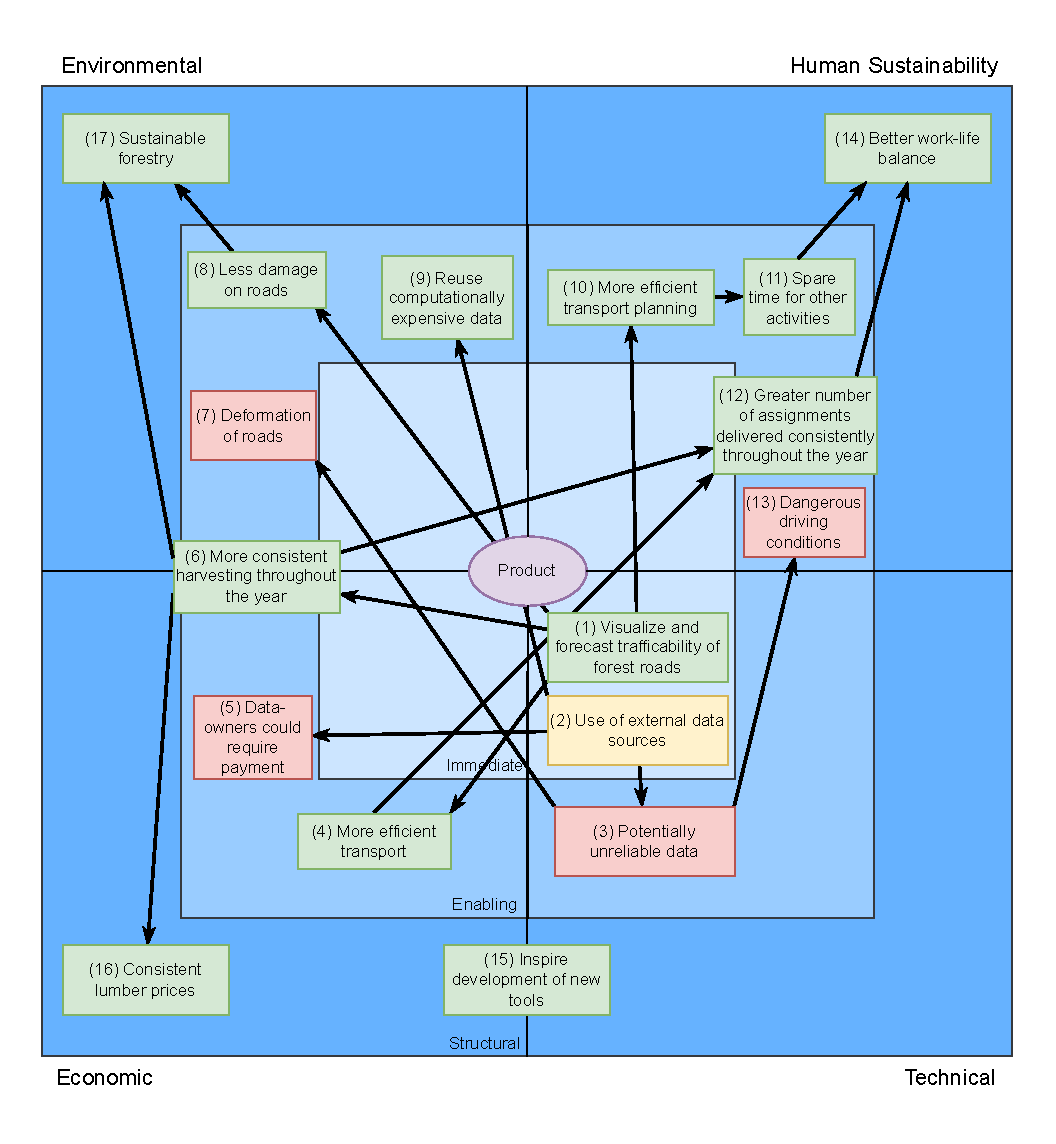
\includegraphics[width=0.8\linewidth]{figures/susaf.pdf}
    \caption{Sustainability Awareness Diagram}
    \label{fig:susafdiagram}
\end{figure}

From the analysis, two chains of effects leading to structural change were found. An immediate effect of the product is that it provides a way to visualize and forecast trafficability of forest roads. This enables more consistent harvesting throughout the year, which could lead to the structural change of more consistent lumber prices and sustainable forestry. The other chain also starts from the same immediate effect and leads to sustainable forestry, but by enabling less damage on roads.

Some potentially negative chains of effects were also identified. The reliance on external data sources introduces certain risks. For instance, data providers may begin charging for access, which could impact the product's long-term viability. Additionally, since the data is controlled by third parties, it may be incomplete, outdated, or otherwise unreliable. This could, in turn, lead to incorrect assessments of road conditions, potentially resulting in hazardous driving situations or damage to forestry roads. The different chains of effects are detailed in \autoref{tab:chain_of_effects}.

\begin{table}[h]
    \centering
    \renewcommand{\arraystretch}{1}
    \begin{tabularx}{\textwidth}{|l|X|l|l|l|}
        \hline
        \rowcolor{gray!20}
        \textbf{ID} & \textbf{Effect} & \textbf{Level} & \textbf{Affects} & \textbf{$+/-$} \\ 
        \hline
         1 & Visualize and forecast trafficability of forest roads & Immediate & 4, 6, 8, 10 & $+$ \\
         \hline
         2 & Use of external data sources & Immediate & 3, 5, 9 & $=$ \\
         \hline
         3 & Potentially unreliable data & Enabling & 7, 13 & $-$ \\
         \hline
         4 & More efficient transport & Enabling & 12 & $+$ \\
         \hline
         5 & Data owners could require payment & Enabling &  & $-$ \\
         \hline
         6 & More consistent harvesting throughout the year & Enabling & 12, 16, 17 & $+$ \\
         \hline
         7 & Deformation of roads & Enabling & & $-$ \\
         \hline
         8 & Less damage on roads & Enabling & 16 & $+$ \\
         \hline
         9 & Reuse of computationally expensive data & Enabling & & $+$ \\
         \hline
         10 & More efficient transport planning & Enabling & 11 & $+$ \\
         \hline
         11 & Spare time for other activities & Enabling & 14 & $+$ \\
         \hline
         12 & Greater number of assignments delivered consistently over the year & Enabling & 14 & $+$ \\
         \hline
         13 & Dangerous driving conditions & Enabling & & $-$ \\
         \hline
         14 & Better work-life balance & Structural & & $+$ \\
         \hline
         15 & Inspire development of new tools (Affected by all positive effects) & Structural & & $+$ \\
         \hline
         16 & Consistent lumber prices & Structural & & $+$ \\
         \hline
         17 & Sustainable forestry & Structural & & $+$ \\
         \hline
    \end{tabularx}
    \caption{Table showing chain of effects}
    \label{tab:chain_of_effects}
\end{table}

From this analysis, the product's effect on sustainability can also be related to the UN \acrshort{sdg}s. These goals are split into three dimensions, economic, social, and environmental. \textcolor{orange}{nevne at wedding cake er brukt?}

\begin{comment}
LENKE FRA PETER: https://www.ntnu.edu/web/excited/sustainability-in-computing-education
% Står litt om skogkurs og bærekraft: https://s46339.pcdn.co/wp-content/uploads/Sluttrapport.pdf
% OG HER: https://skogkurs.no/fagartikler/baerekraftige-metoder-og-kompetanse-i-skogsmaskinbransjen-kurs-kommer/ ->
- mer lukkede hogstformer og mindre bruk av flatehogst 
- **lavere drivstofforbruk og smartere kjøring med skogsmaskin** 
    - **lavere førerbelastning**
    - **mindre terrengslitasje**
    - **høyere produktivitet**
- produsere tømmer som er mest mulig tilpasset industriens behov 
- **videreutvikle teknologi for driftsoppfølging og førerstøtte for maskinførerne** 

###########################
FNs Bærekraftsmål som virker relevante (KANSKJE SAMMENLIGN MED HVA NORGE GJØR I DAG?):

- 9
- 12 (?) VIRKER SOM DEN FOKUSERER MEST PÅ UTVIKLINGSLAND?
- 15 (?)
\end{comment}

\subsubsection{Economic}\label{subsubsec:discussion:product:sustainability:economic}

% 9.5 Enhance scientific research, upgrade the technological capabilities of industrial sectors in all countries, ...
%\textcolor{orange}{SDG: 8 (8.2, 8.4), 9 (9.5)}
%\textcolor{orange}{Your product contributes directly to improved economic productivity by making forestry logistics more data-driven and efficient (effects 1, 4, 6, 11, 13). By enabling better forecasting of trafficability, it supports more consistent harvesting and delivery schedules, which benefits forestry operations financially and operationally. This aligns with Goal 8.2, as you're using digital innovation to enhance productivity in a traditional sector.\\ The reuse of data (effect 10) and reduction in road damage (effect 9) both support resource efficiency (Goal 8.4), helping reduce unnecessary fuel usage, road maintenance, and inefficient trips.\\The system as a whole enhances technological capability within the forestry sector, directly aligning with Goal 9.5.}

Visualizing the trafficability of forestry roads enhances the efficiency of lumber transport from logging sites by facilitating better planning and decision-making. It reduces uncertainty about the trafficability of specific roads, also helping to prevent damage and deformation caused by driving during unsuitable conditions. These improvements align closely with the United Nations' \acrshort{sdg}s, particularly Goal 8 (Decent Work and Economic Growth) and Goal 9 (Industry, Innovation, and Infrastructure). 

Target 8.2 is the following: "Achieve higher levels of economic productivity through diversification, technological upgrading and innovation, including through a focus on high-value added and labour-intensive sectors", with the indicator of annual growth rate of real GDP per employed person \cite{sdgsgoals}. Effect number 4, 6, and 12 (see \autoref{tab:chain_of_effects}) are relevant to this indicator by making parts of the forestry industry more efficient, by upgrading the technological tools used. Similarly, target 9.5 is: "Enhance scientific research, upgrade the technological capabilities of industrial sectors in all countries, ...", with the indicators of research and development expenditure and amount of researchers per million inhabitants \cite{sdgsgoals}. A possible side-effect of all positive effects is that they inspire industrial sectors to increase expenditure and focus on research and development of data-driven tools make specific tasks more effective, as described in effect 15.

\subsubsection{Social}

\textcolor{orange}{Kanskje si man mangler her, og nevn hvordan det kunne forbedres. SDG: 10 (10.2 [usability]), 3.6 [trafikkulykker], 8 [stable life-work balance?] skriv om første setning?}

By making the planning of transport routes more efficient the product may contribute to more predictable work schedules and a reduced need for overtime, leading to a better work-life balance, as described in effect number 14. These improvements relate to both \acrshort{sdg} 8 (Decent Work and Economic Growth) and \acrshort{sdg} 3 (Good Health and Well-Being). A better work-life balance supports healthier working conditions and can improve mental well-being. This is especially relevant in Norway, where recent editions of the World Happiness Report indicate a decline in overall happiness. Increased stress at work can negatively affect mental health and, by extension, impact national well-being scores \cite{sdg3no}.

\subsubsection{Environmental}

\textcolor{orange}{SDG: 15 (15.2, 15.b), 12 (12.2). Nevnt mulig "Rebound effect" fra at det blir lettere å frakte tømmer, kanskje?}

As Effect 6 from the \acrshort{susaf} says, the product contributes to more consistent harvesting and reforestation practices, supporting the development of sustainable forestry. This aligns with the United Nations' \acrshort{sdg} 15.2, which focuses on promoting sustainable management of all types of forests \cite{sdgsgoals}.

Furthermore, the product supports \acrshort{sdg} 12, particularly target 12.2, which emphasizes the sustainable management and efficient use of natural resources \cite{sdgsgoals}. By reducing road damage through better trafficability planning (effect 8), the product also helps prevent unnecessary wear on transport vehicles and minimizes environmental disturbance caused by repeated repairs or rerouting.

As stated in \autoref{subsubsec:discussion:product:sustainability:economic}, the product may inspire further innovation in the forestry sector. This applies to \acrshort{sdg} 15.b, which calls for mobilizing resources to finance sustainable forest management and promote the development of related technologies and initiatives \cite{sdgsgoals}.

% Jevons paradox https://en.wikipedia.org/wiki/Jevons_paradox
% Mer effektiv, mer etterspørsel -> Mer hogst -> if {ikke blir planta ny skog} = unsustaiable forestry

Not all aspects of the product necessarily contribute to greater sustainability. A relevant consideration is the Jevons paradox, which  occurs when technological advancements make a resource more efficient to use, however, as the cost of using the resource drops, if the price is highly elastic, this results in overall demand increasing, causing total resource consumption to rise \cite{jevonsparadoxwiki}. In this context, by making lumber harvesting more efficient, the product may contribute to lower prices and increased demand for lumber. If this demand is not met with a corresponding increase in reforestation efforts, it could result in unsustainable forestry practices.

\subsection{Future Work}

Throughout the project, the application has evolved with the most prioritized features being implemented. The group has considered various ideas for additional functionality, and we have also received valuable feedback from the Product Owner and other stakeholders. However, due to time constraints, several of these suggestions were not incorporated during the project period. Below is a list of some of these ideas:

\begin{itemize}
    \item \textbf{User Guide}: Include a user guide on the website on how to use it.
    \item \textbf{Mobile Application}: Implement for better use on mobile devices.
    \item \textbf{Offline Mode}: Download map data for a set time period and location. This requires that the application is deployed as a mobile or desktop application.
    \item \textbf{Export Data}: Let the user export data (e.g., CSV) for use in other applications.
    \item \textbf{Machine Learning}: Use machine learning to improve predictions about trafficability.
    \item \textbf{Notification System}: Send notifications or webhooks for changes in trafficability or weather.
    \item \textbf{Reporting System}: Generate reports that show the state of forestry roads in a period. Could include diagrams, statistics, etc.
    \item \textbf{Better Accessibility}: Better universal design. Color-blind modes and accessibility controls.
    \item \textbf{Hour Picker}: Updating the Data Picker component to also be able to select the hour of day could be useful if conditions vary a lot hourly, for example when the temperature oscillates around \qty{0}{\celsius} throughout the day. \textcolor{orange}{Noe mer om at veien blir bedre når den er kald, selvom frosten ikke er dyp.}
    \item \textbf{Performance}: Ways of improving performance. Using WebGL for rendering of vectors. This does require newer hardware/browsers) også backend opti). Performance testing flere brukere samtidig?
    \item \textbf{User Testing}: Conduct structured user testing.
    \item \textbf{Integrate with Existing Solutions}: Use with existing solutions like VSYS. 
    \item \textbf{Filtering}: Better ways of filtering by roads and locations.
\end{itemize}

\begin{comment}
    - User Guide
    - Offline Mode (download a map with data)
    - Mobile (har vi alt?)
    - Export Data
    - Machine Learning
    - Notification System
    - (Condition reporting system, si at en trucker kan si at denne veien var dårlig, typ det DF mente)
    - Better Accessibility (e.g. color-blind modes)
    - Hour picker (for mer detaljert data for spesifikke tidspunk, f.eks. om en sjåfør skal kjøre om natten)
    - More Optimization?
        - WebGL for rendering of vectors (downside?: does require newer hardware/browsers)
    - Code Quality, what to add to improve?
\end{comment}

\chapter{Conclusion}\label{chap:conclusion}

\textcolor{orange}{NOE TEKST}
\begin{comment}
    FRA PRESENTASJON OM KONKLUSJON:
    1. Gå tilbake til temaet
    2. Gjenoppgi hovedpåstanden eller gjenta problemstillingen
    3. Oppsummering av ideene som er diskutert
    4. Oppsummerende sluttpoeng:
        - Forsterke hovedbudskapet
        - Gi en tankevekker eller refleksjon
        - Peke på videre implikasjoner
\end{comment}

\section{Summary}\label{sec:summary}

\textcolor{orange}{NOE TEKST}

\section{Final Thoughts}\label{sec:finalthoughts}

\textcolor{orange}{NOE TEKST}


\chapter*{\bibname}
\printbibliography[heading=none]

% First paper

\begin{paper}{papers/landes1951scrutiny.pdf}{paper:scrutiny}
    Here, you may add a description of the paper, an illustration, or just give the bibliographic reference:
    \begin{quote}
        \fullcite{landes1951scrutiny}
    \end{quote}
    Or you may leave it empty, if you like.
\end{paper}

% Second paper etc.

\appendix
\chapter{Project Plan}
\label{appendix:project_plan}
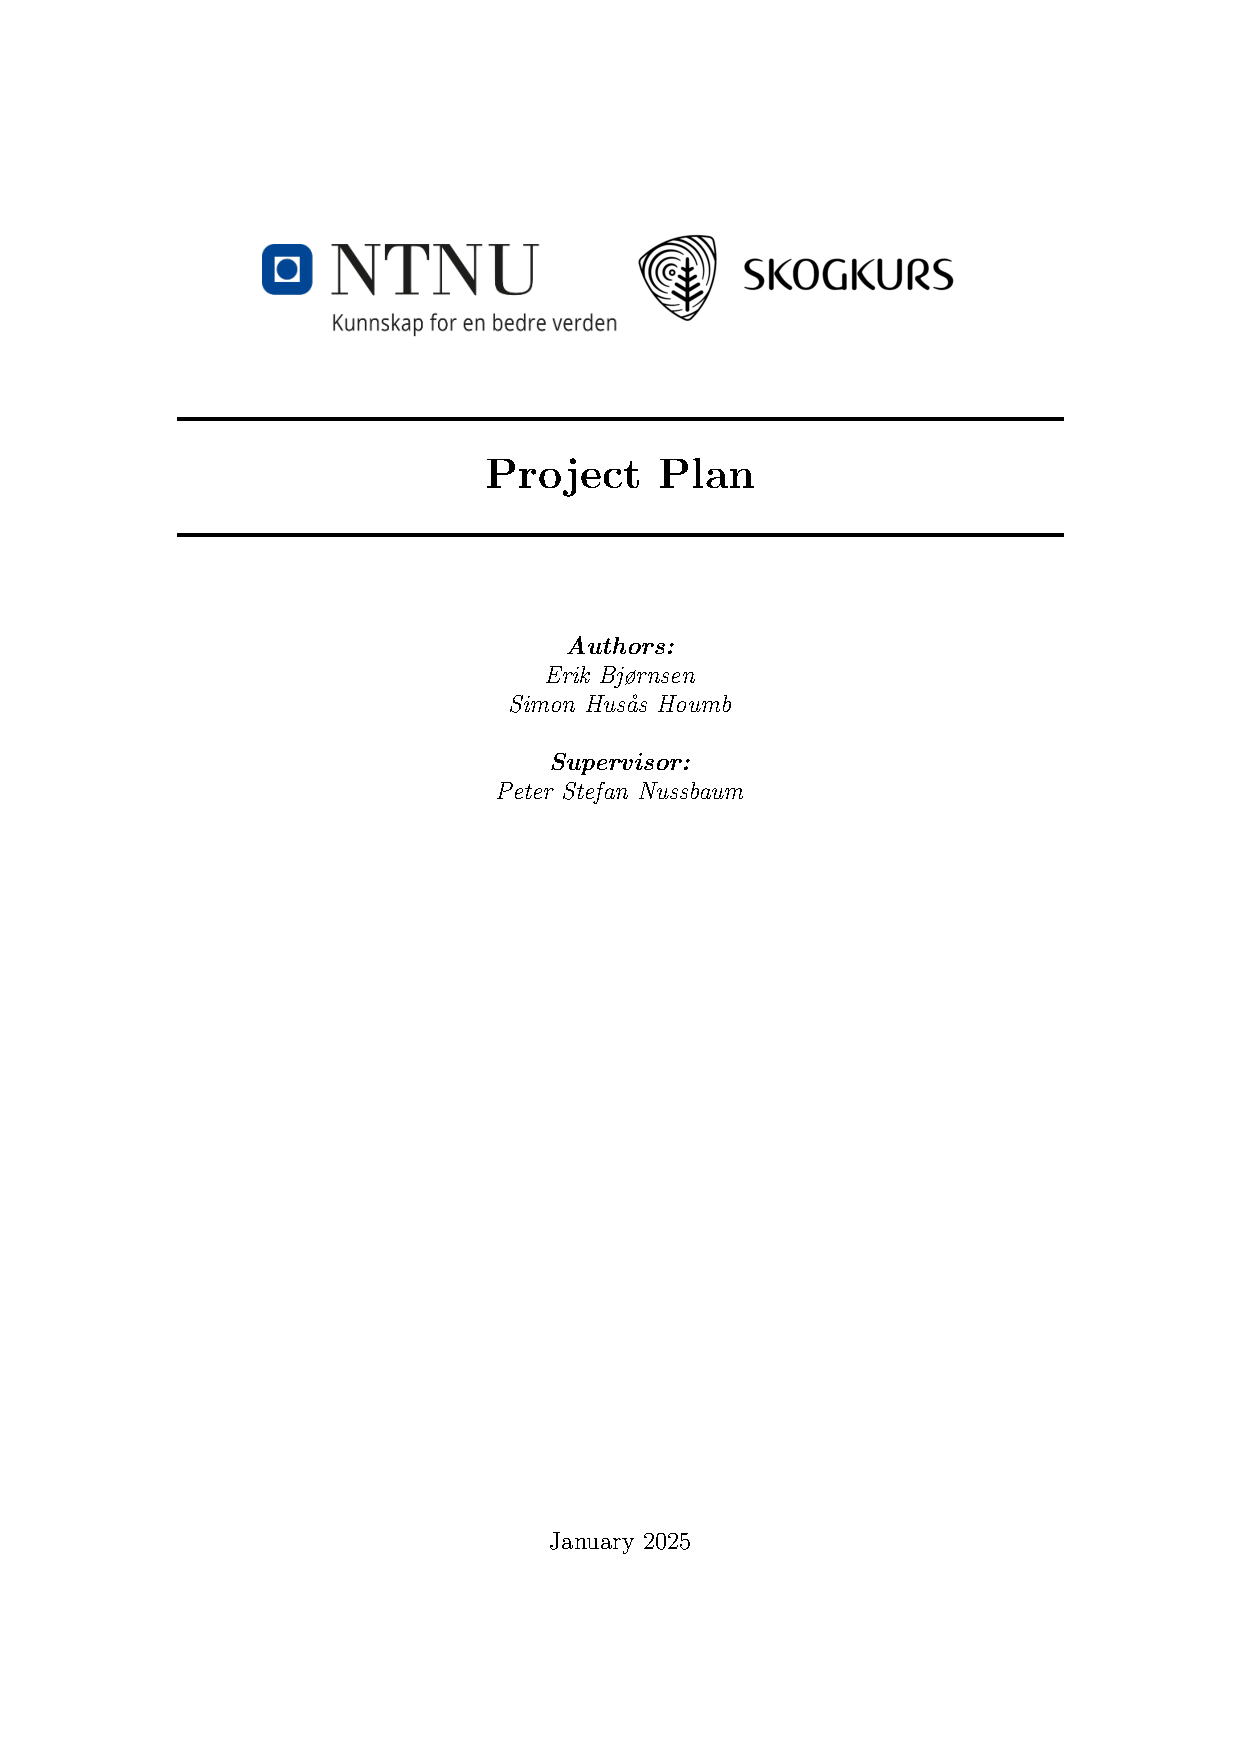
\includepdf[pages=-]{appendices/Skogkurs_Bachelor_Project_Plan_noAppendix}
\chapter{Group Contract}
\label{appendix:group_contract}
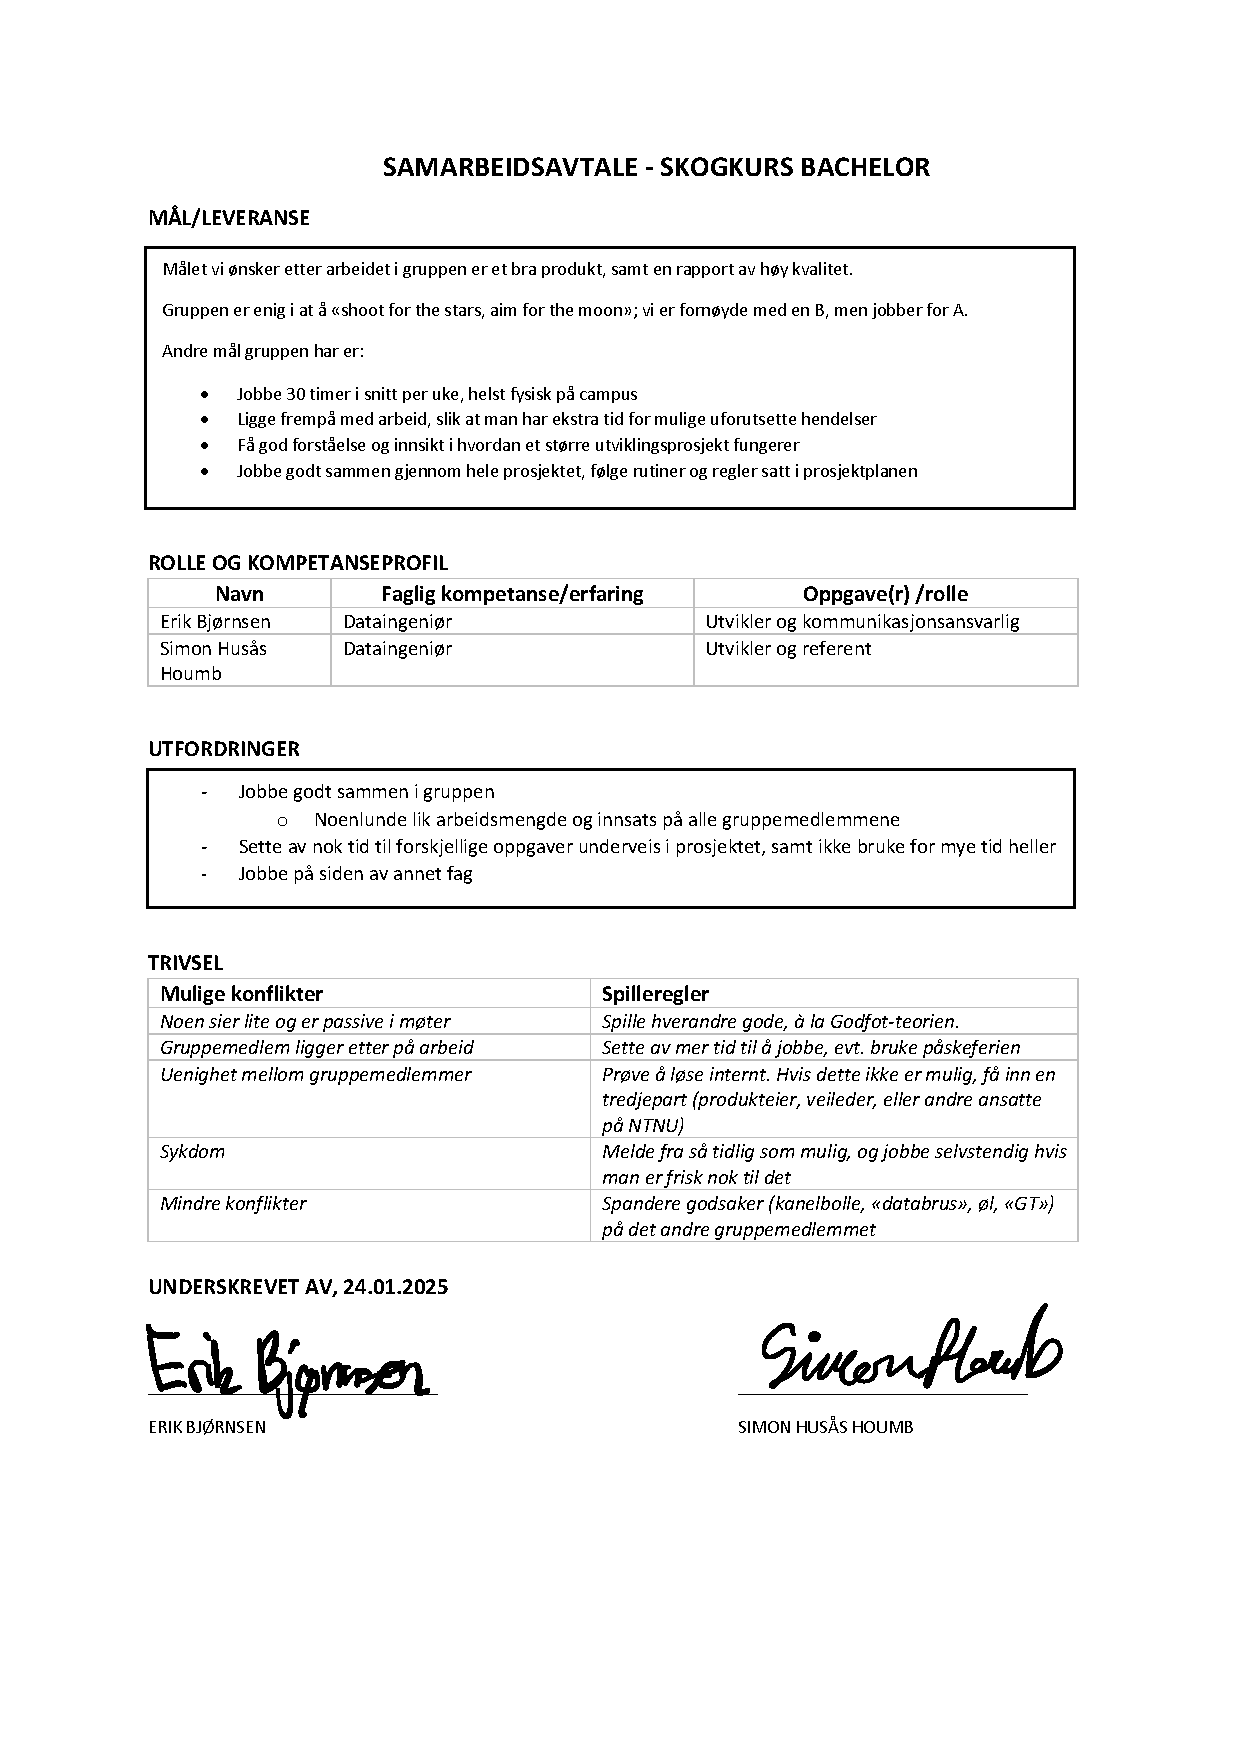
\includepdf[pages=-]{appendices/bachelor_skogkurs_samarbeidsavtale}
\chapter{Project Agreement}
\label{appendix:project_agreement}
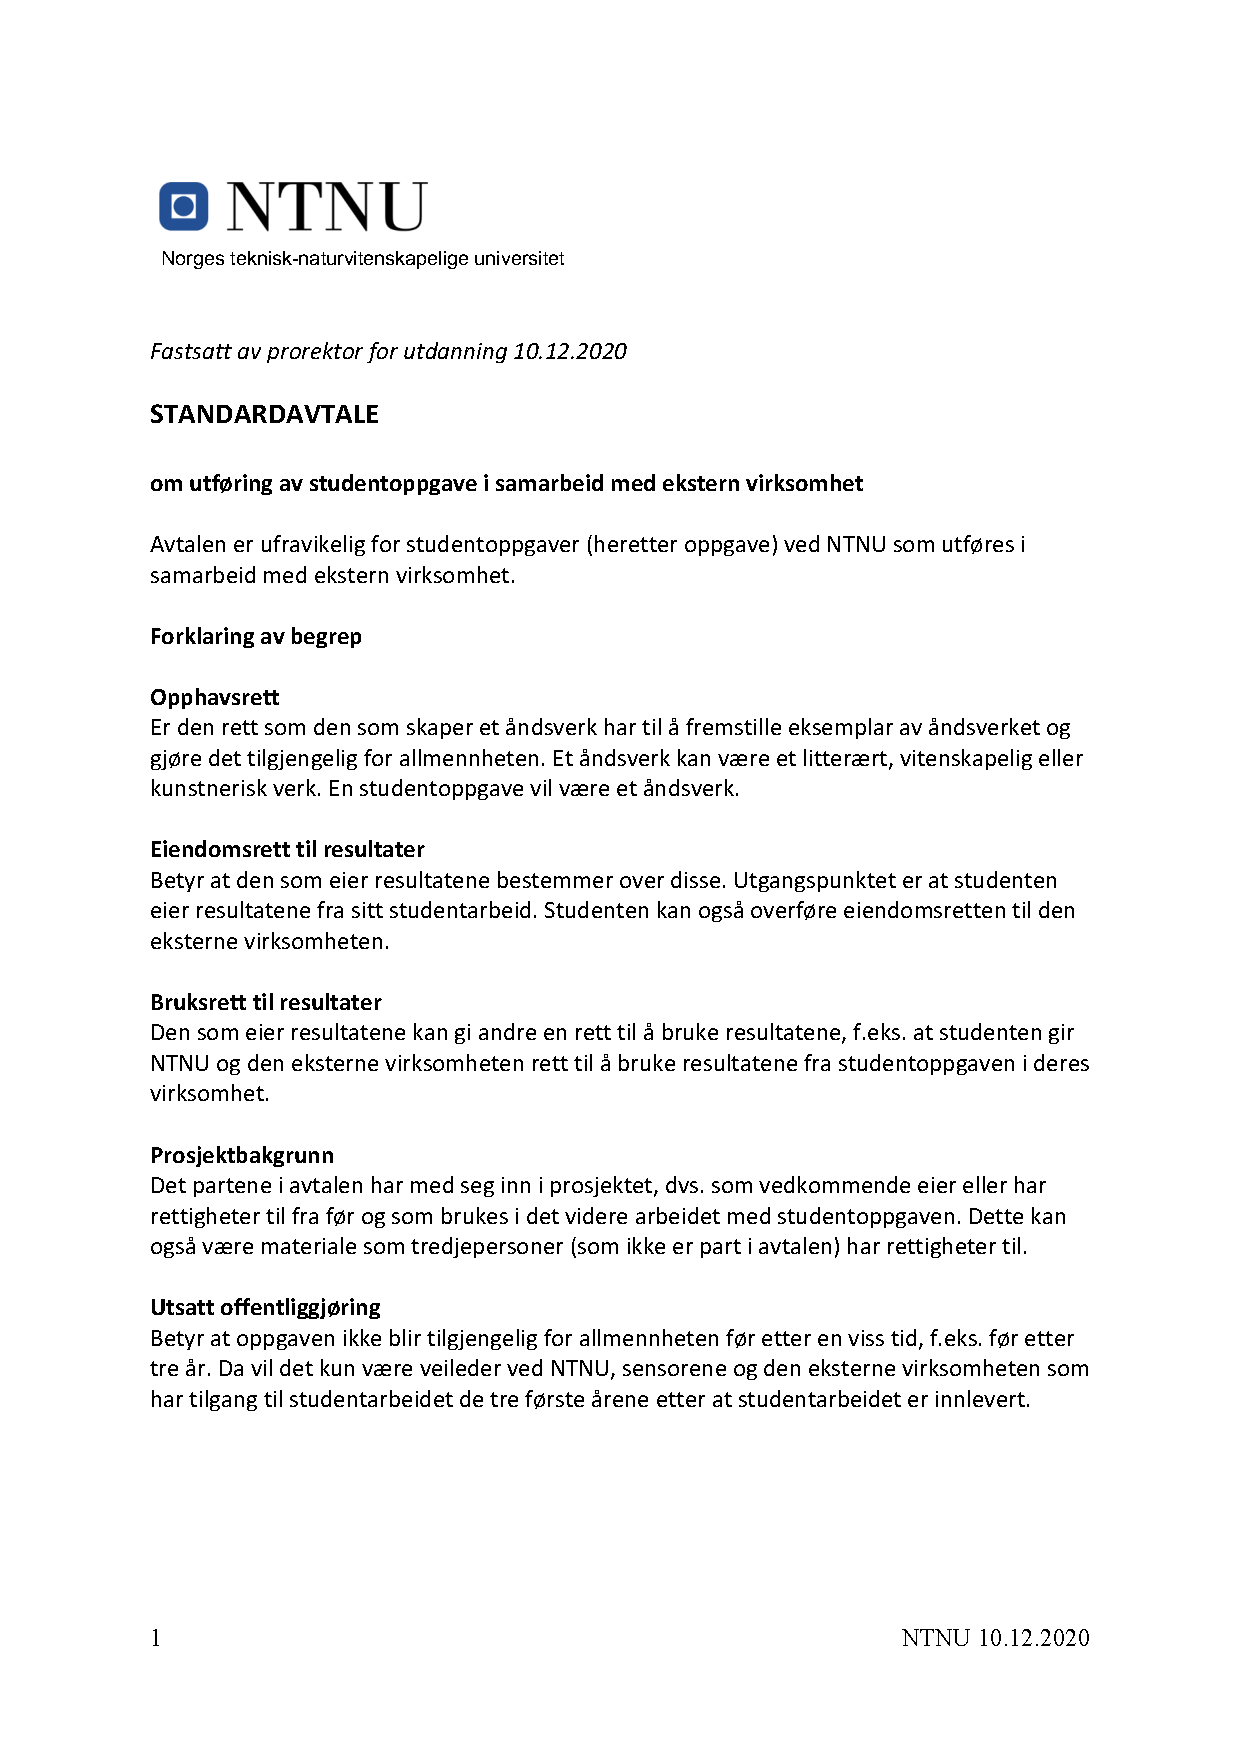
\includepdf[pages=-]{appendices/standardavtale_skogkurs_bachelor.pdf}
\chapter{Task Description}
\label{appendix:task_description}
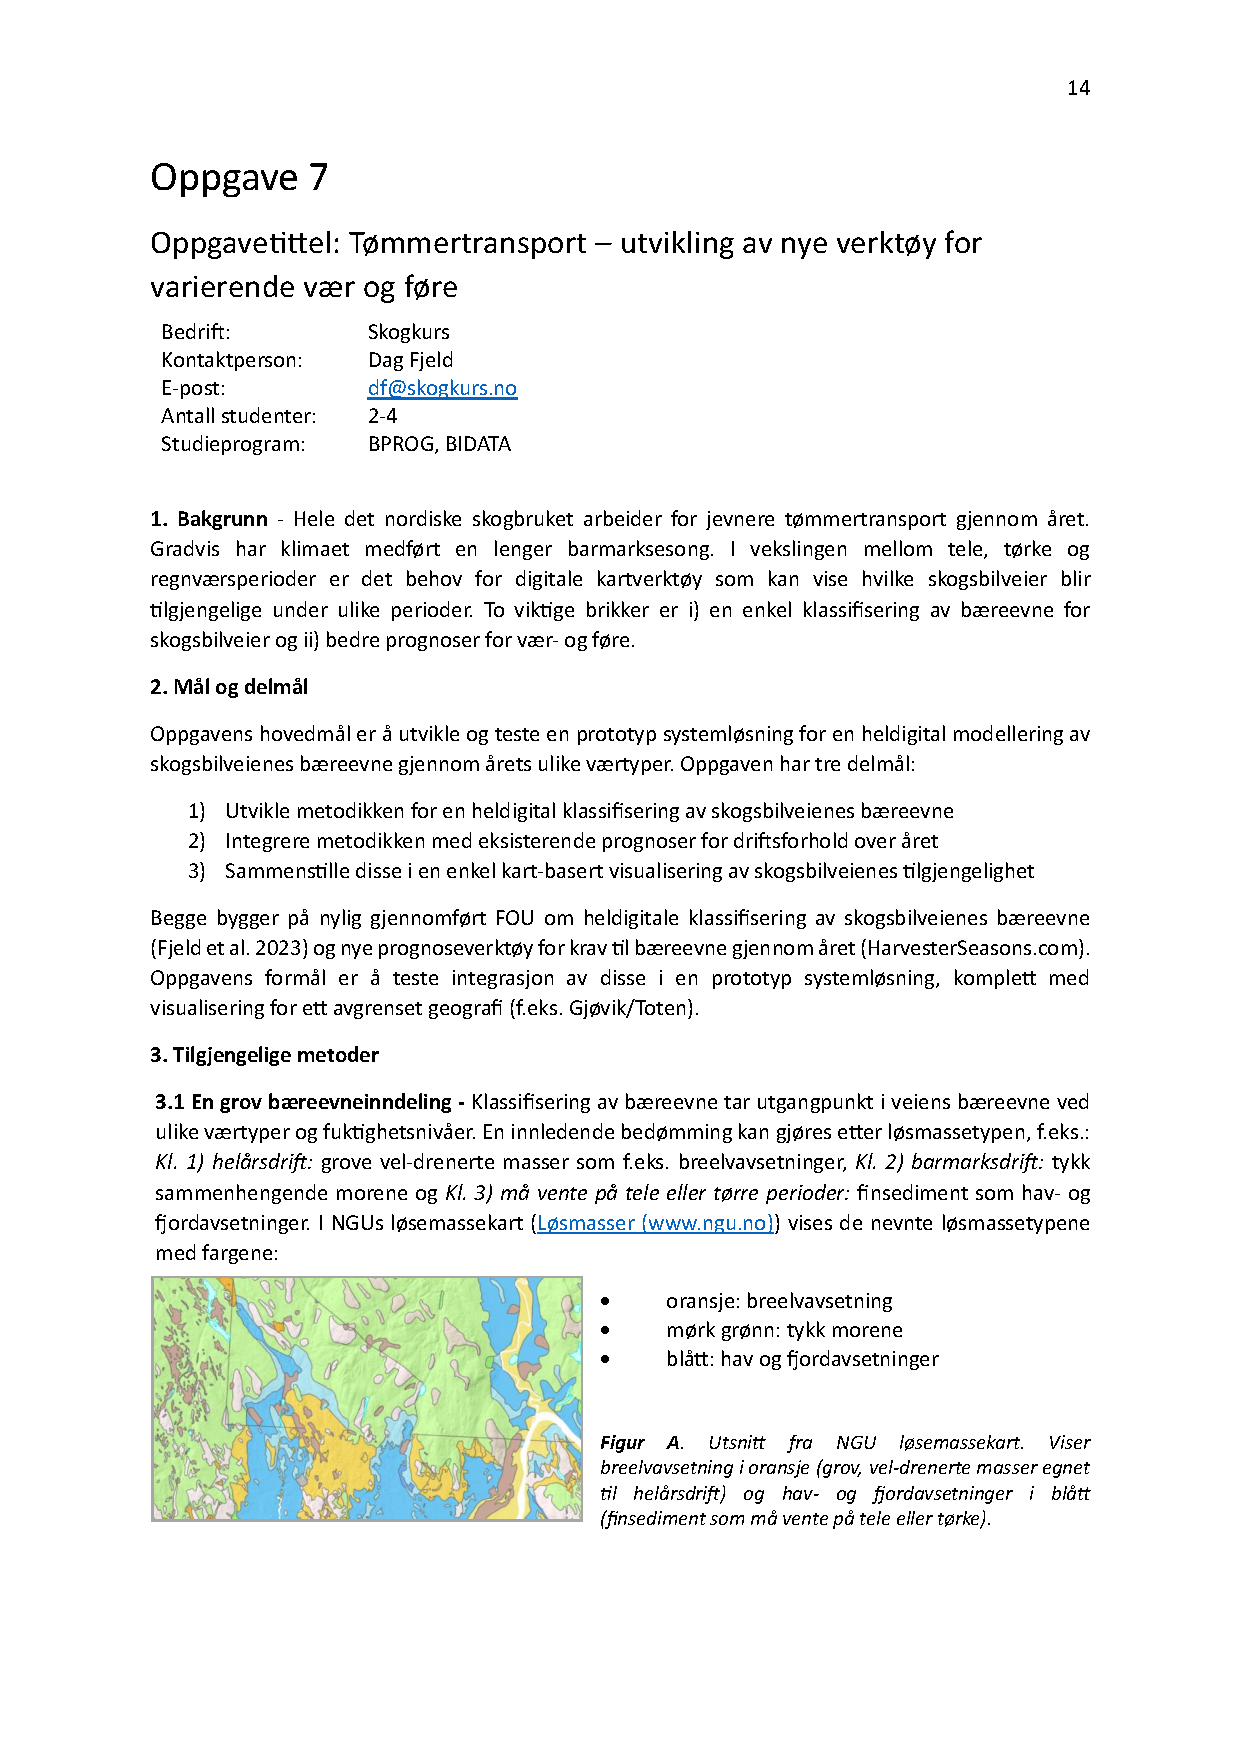
\includepdf[pages=-]{appendices/SKOGKURS_BACHELOROPPGAVE.pdf}
\chapter{Meeting Minutes}
\label{appendix:meeting_minutes}
\section*{Møte med Veileder: 2025-01-14}
\begin{itemize}
\item
  Kjernetid: 9-15, 6 timer hver dag. Vi har forelesning på mandager
  14-16 og onsdager 10-12, og gruppearbeid i samme fag som vil ta litt
  av kjernetiden første ukene.
\item
  Møte: Ukentlig med veileder, og annen hver uke med oppdragsgiver?
\item
  Ha klart spørsmål om kravspesifikasjon til Dag
\end{itemize}

\section*{Møte med Veileder og
Produkteier: 2025-01-21}

\subsection*{Agenda}
\begin{itemize}
\item
  Referere til andre sine bacheloroppgaver i prosjektplan?
\item
  Flere MVPer? Vi har nå tenkte 1 MVP midt i mars for user-testing
\item
  Få en gjennomgang til av
\item
  Annen data og utregning
\item
  NASA SMAP og ESA Sentinel-1
\item
  Hvilke data skal brukes
\item
  Hvordan få prognose frem i tid, bruke verktøy som allerede finnes
  eller lage selv?
\item
  Prosjektplan
\item
  Constraints
\item
  Delimitation (er Norge for stort område å fokusere på)
\end{itemize}

\begin{enumerate}
\item
  Dag
\item
  Kanskje Dag kan si litt om oppgaven til Peter
\item
  Gå gjennom det vi har hittil (prosjektplan, gantt)
\item
  Spørsmål
\end{enumerate}

\subsection*{Notater}
\textbf{Product \& Impact Goals:} 
\begin{itemize}
    \item Ligger på linje med Skogkurs'
forventninger
\item Impact (reduced uncertainty)
\end{itemize}
\textbf{Brukere:} 
\begin{itemize}
    \item \emph{Transportleder}
    \item Sjåfører
    \item ``Personer med kunnskap i feltet''
\end{itemize}
\textbf{Prognose:} 1-2 uker\\
\textbf{Fargekoding av vei (trafikklys):} Rød, gul, grønn\\
\textbf{Område:} Begrenset område - Gjøvik, steder det faktisk kan
bruke. For mye data.\\
\textbf{Bruk av data / variabler (begrensning):}
\begin{itemize}
    \item (Ikke konkret rett valg av data, mål å få testet at et produkt fungerer)
    \item \emph{Løsmasser}
    \item Markfuktighet
    \item Teledyp
    \item Grunnvannstilstand
    \item Skogbilveier
    \item Variere for forskjellige områder hvor det er relevant
    \item Evt. snitt data hvor flere lag brukes
    \item (ikke tenk på vekt av last)
\end{itemize}

\textbf{Brukertesting:} \\
\begin{itemize}
    \item Tidlig Wireframe slik at for teste tidlig versjon
    \item For transportledere, hjelp fra Skogkurs
\end{itemize}
\textbf{Begynne med å definere data som trengs og skal brukes i februar}
\begin{itemize}
    \item Nibio skogsportal (WMS)
    \item Traktor og skogsbilvei
    \item senorge - raster
\end{itemize}


\section*{Møte med Veileder: 2025-01-28}

\subsection*{Agenda:}
\begin{itemize}

\item
  Referere til andre sine bacheloroppgaver i prosjektplan?
\item
  Hvor spesifikt skal produktmål være?
\item
  I avsnitt om scrum, skal vi skrive om hvorfor vi ikke valgte de andre
  metodene?
\item
  Scope: burde man nevne data fra rapportene til Dag Fjeld?
\item
  Gjennomgang av scope, domain og task desc.
\end{itemize}

\subsection*{Notat:}

\begin{itemize}
\item
  Fokus på rapport, få med det som gikk bra, og hva som var utfordrende
\item
  Kartlegging i februar (data)
\item
  Finne kriteriene for data som skal eller kan brukes for å
  tilfredsstille krav
\item
  Se gjennom rapportene til D. Fjeld (abstrakt, introduksjon,
  konklusjon)

  \begin{itemize}
  \item
    Se om andre rapporter er referert
  \end{itemize}
\item
  Hvor mange uker satt av for rapport?:

  \begin{itemize}
  \item
    Kreves litt mer tid, men finn balanse
  \end{itemize}
\item
  Få teksten lest over av noen eksterne (andre studenter, familie?)

  \begin{itemize}
  \item
    Sette av litt tid for finpussing da for at noen skal lese over
  \item
    Passe på å ha en ``rød tråd'' gjennom rapporten, tenke på
    overgangene mellom deler av rapporten
  \end{itemize}
\item
  Kanskje finne lignende bachelor
\item
  Referer til andre oppgaver (ikke kopier rett fra teksten)
\item
  Skrive om SDLC

  \begin{itemize}
  \item
    Vise at man vet om andre metoder
  \item
    men ikke skrive for langt
  \item
    Finne argumenter for valg man har tatt, også andre steder i teksten
  \end{itemize}
\item
  Scope:

  \begin{itemize}
  \item
    Skogsdrift, tungtransport
  \item
    Kart
  \end{itemize}
\item
  Task description:

  \begin{itemize}
  \item
    Steg for å nå målet
  \item
    Analyse av kriterier som trengs for å nå mål
  \item
    Implementasjon av kart og webside
  \end{itemize}
\item
  Impact Goals

  \begin{itemize}
  
  \item
    Kanskje ha med noe om bærekraft, miljø, etc.
  \end{itemize}
\end{itemize}

\section*{Møte med Veileder: 2025-02-04}

\subsection*{Notat}
\begin{itemize}
\item
  Spørre produkteier om dataressurser vi har funnet
\end{itemize}

\section*{Møte med Produkteier: 2025-02-10}

\subsection*{Spørsmål}

\begin{itemize} 
\item
  OpenMeteo Ensemble API

  \begin{itemize}
  \item
    Hvor dyp jordfuktighet er nødvendig?
  \item
    Hvor nøyaktig er OpenMeteo?
  \end{itemize}
\item
  Detaljert info for skogsveg fra NIBIO: \\
  https://kilden.nibio.no/skogsbilveger\_ws/skogsbilveiInfo?sveiid=3407-14-1
\end{itemize}

\subsection*{Notat}

\begin{itemize}
\item
  Når vegen ble bygd: ØKS? Landbruksdirektoratet

  \begin{itemize}
  
  \item
    Kategorisere vegene i klasser
  \item
    Nyere og bedre veier etter 2015
  \end{itemize}
\item
  Hva er vegen bygd av
\item
  Forskjellige høydenivå på veger
\item
  Hvordan bruke soil moisture

  \begin{itemize}
  \item
    Sette klasser
  \end{itemize}
\item
  Grenser for data

  \begin{itemize}
  \item
    Kanskje ha dynamiske grenser (som kan endres av bruker)?
  \item
    Sette grenser ved bruk av historisk data?
  \end{itemize}
\item
  Ha med historisk data, da OpenMeteo kanskje ikke støtter dette.
\end{itemize}

\section*{Møte med Veileder: 2025-02-11}

\subsection*{Agenda}

\begin{itemize}
\item
  Snakke om samtalen med Dag Fjeld
\item
  Plakat/rapportmal 
\end{itemize}

\subsection*{Notat}
\begin{itemize}
    \item
      Skal spørre Pål om rapportmal
    \item
      Notere ned detaljer allerede for å ha med i den endelige rapporten
    \item
      Får mal på lynkurs, kan også finne på nett
    \item
      Info blir også gitt om plakat senere på seminar om presentasjon
\end{itemize}

\section*{Møte med Veileder: 2025-02-20}

\subsection*{Agenda}

\begin{itemize}
\item
  Vise fremgang av webside
\end{itemize}

\subsection*{Notat}

\begin{itemize}
    \item Husk å notere vanskeligheter underveis for å ha med i rapporten senere
\end{itemize}

\section*{Møte med Veileder: 2025-02-24}

\subsection*{Agenda}
\begin{itemize}
\item
  Vise fremgang av webside før møte med produkteier
\end{itemize}


\section*{Møte med Produkteier: 2025-02-25}

\subsection*{Agenda}

\begin{itemize}
\item
  Vise frem proto-prototype av webside
\end{itemize}
\subsection*{Notat}
\begin{itemize}
\item
  Copernicus, evt. prognose
\item
  Få implementert open-meteo soil moisture / soil temperature
\item
  Teledyp grenser:

  \begin{itemize}
  \item
    Både 0-7cm og 7-28cm jordtemperatur er null = grønt lys
  \item
    Jordfuktighet forskjell mellom forskjellige jordarter
  \end{itemize}
\end{itemize}

\section*{Møte med Veileder: 2025-03-04}

\subsection*{Agenda}

\begin{itemize}
\item
  Snakke om møte med produkteier forrige uke
\item
  Hva planen er fremover for denne sprinten
\end{itemize}

\subsection*{Notat}

\begin{itemize}
\item
  For klassifisering av skogsbilveg

  \begin{itemize}
  \item
    Se skiforeningens side
  \end{itemize}
\item
  Få med utfordringer, blindveier i prosessen etc. i rapport
\end{itemize}

\section*{Møte med Veileder: 2025-03-13}

\subsection*{Agenda}

\begin{itemize}
\item
  Fullt fokus på bacheloroppgaven fra nå
\end{itemize}

\subsection*{Notat}

\begin{itemize}
\item
  Se rapportskrivings krasjkurs
\item
  Rapportskrivingskurs 27. Mars
\item
  Første utkast av rapport til påske f.eks. tirsdag 8. april, gi til
  veileder for tilbakemelding
\item
  Tilbakemelding på utkast etter påske tirsdag 22. april
\end{itemize}

\section*{Møte med Veileder: 2025-03-18}

\subsection*{Agenda}
\begin{itemize}
\item
  Forside til rapporten, skal vi ha med egen eller blir den generert ved
  innlevering
\item
  Eksempler på ``A''-rapporter
\item
  Hva burde være med av kapitler, særlig introduksjon. F.eks. skal ikke
  ha med gruppebakgrunn eller noe personlig om gruppen (ifølge Hjelmås)
\item
  Mellomrom eller innrykk mellom avsnitt
\item
  Referanse har tomt parantes hvis man ikke legger til dato for når
  siden ble sist oppdatert. Er dette nødvendig og hvis det ikke er
  oppgitt kan man bruke ``n.d.'' (no date)
\item
  Chapter vs.~Section. Virker litt unaturlig at det står Chapter 1, 2, 3
  osv.
\item
  Latex tar med forfatter og tittel på hver partall side, f.eks.
  ``erbj\&simonhou@NTNU: Lumber transport'' er dette meningen?
\item
  Er det relevant å ta med som utfordring at tidsfordeling med et annet
  fag på siden av bachelor
\end{itemize}
  
\subsection*{Notat}
\begin{itemize}
\item
  Kan ta med i rapporten at man finner frem til løsninger ved å sparre
  med AI.
\item
  Forside til rapporten, skal vi ha med egen eller blir den generert ved
  innlevering

  \begin{itemize}
  \item
    \emph{Får svar før innlevering.}
  \end{itemize}
\item
  Eksempler på ``A''-rapporter

  \begin{itemize}
  \item
  \end{itemize}
\item
  Hva burde være med av kapitler, særlig introduksjon. F.eks. skal ikke
  ha med gruppebakgrunn eller noe personlig om gruppen (ifølge Hjelmås)

  \begin{itemize}
  \item
    \emph{Hvis man skal ta det med så hold det kort.}
  \item
    \emph{Er mulig å få A selv om man tar med.}
  \end{itemize}
\item
  Mellomrom eller innrykk mellom avsnitt

  \begin{itemize}
  \item
    \emph{Mellomrom}
  \end{itemize}
\item
  Referanse har tomt parentes hvis man ikke legger til dato for når
  siden ble sist oppdatert. Er dette nødvendig og hvis det ikke er
  oppgitt kan man bruke ``n.d.'' (no date)?

  \begin{itemize}
  
  \item
    \emph{Prøv å fjern parentesen hvis ingen dato er oppgitt istedenfor
    å bruke n.d. eller no date}
  \end{itemize}
\item
  Chapter vs.~Section. Virker litt unaturlig at det står Chapter 1, 2, 3
  osv.

  \begin{itemize}
  
  \item
    \emph{Ja, chapter skal ytterst}
  \end{itemize}
\item
  Latex tar med forfatter og tittel på hver partall side, f.eks.
  ``erbj\&simonhou@NTNU: Lumber transport'' er dette meningen?

  \begin{itemize}
  
  \item
    \emph{At kapittel står er fint, men må ikke ha med forfatter
    og/eller tittel.}
  \end{itemize}
\item
  Er det relevant å ta med som utfordring at tidsfordeling med et annet
  fag på siden av bachelor. Også med tidsfordeling om at vi kun er 2 i
  gruppen.

  \begin{itemize}
  
  \item
    \emph{Hvis man kan ta med på en bra måt så ta med på en objektiv
    måte, ikke for spesifikt.}
  \item
    \emph{Ikke nevn følelser (adjektiver), ikke spesifiser 2 i gruppen
    (sensor vet det). Heller nevn at man var litt for optimistisk på
    tiden man hadde.}
  \item
    \emph{Trenger kanskje ikke nevne hvis det ikke ble lovet i planen
    eller at det ikke var et krav fra produkteier.}
  \end{itemize}
\item
  Ha tekst for hvert nye kapittel (som forklarer innholdet for
  kapitellet). Hvis man er i et senere kapittelet kan denne setningen
  gjerne inneholde et slags\\
\item
  Vær flink til å ha med figurer for å forklare prinsipper eller hvordan
  produktet fungerer, samt selve prossesen av prosjektet.

  \begin{itemize}
  \item
    Figurer er også fint å bruke i presentasjonen
  \end{itemize}
\item
  Universell Utforming burde tas med, f.eks. ha med spørsmål på
  brukertesting.

  \begin{itemize}
  \item
    Hvis man ikke finner en perfekt løsning for f.eks. design, så nevn
    det i rapport uansett. Eks. fargeblindhet
  \end{itemize}
\end{itemize}
\chapter{Use Case Specifications}
\label{appendix:use_case_specifications}

\begin{table}[h]
    \centering
    \renewcommand{\arraystretch}{1.5}
    \begin{tabularx}{\textwidth}{|l|X|}
        \hline
        \rowcolor{gray!20}
        \textbf{Use Case Name} & Toggle Map Layer \\
        \hline
        \textbf{Actor(s)} & User \\
        \hline
        \textbf{Description} & The user can toggle specific map layers to control the visibility of different map layers. This functionality allows users to select from various map layers. The selected layer is then displayed, and relevant information is shown in the map legend sidebar. \\
        \hline
        \textbf{Priority} & High \\
        \hline
        \textbf{Pre-Condition(s)} & The user must have a stable internet connection and the website open. The website and server and map server must be deployed and running.\\
        \hline
        \textbf{Post-Condition(s)} & The map will be updated with the specific map layer that was toggled. The map legend will also be visible in the legend sidebar. \\
        \hline
        \textbf{Basic Path} &  
        \begin{enumerate}[label=,left=0pt]
            \item 1. User presses the map layer ("kartlag") button to open the map layer sidebar.
            \item 2. User clicks the toggle button for the specific map layer to toggle.
            \item 3. The system updates the map with the selected layer.
        \end{enumerate} \\
        \hline
        \textbf{Exception Path} & 
        \begin{enumerate}[label=,left=0pt]
            \item 0. User does not have a stable internet connection and can not connect to the website.
            \item 2a. Either the backend server or the map server is not responding, and no map data is received.
        \end{enumerate} \\
        \hline
    \end{tabularx}
    \caption[Use Case Specification: Toggle Map Layer]{Use case for toggling a map layer.}
    \label{tab:use_case_toggle_layer_appendix}
\end{table}

\begin{table}[h]
    \centering
    \renewcommand{\arraystretch}{1.5}
    \begin{tabularx}{\textwidth}{|l|X|}
        \hline
        \rowcolor{gray!20}
        \textbf{Use Case Name} & Show Map Legend \\
        \hline
        \textbf{Actor(s)} & User \\
        \hline
        \textbf{Description} & The user can show legends for the map layers that are toggled on. \\
        \hline
        \textbf{Priority} & Medium \\
        \hline
        \textbf{Pre-Condition(s)} & The user must have a stable internet connection and the website open. The website and server and map server must be deployed and running. The map layer for the specific legend must be toggled before the legend is visible. \\
        \hline
        \textbf{Post-Condition(s)} & The legend sidebar will contain the legend for the toggled map layers. If no map layer is toggled, it will be empty. \\
        \hline
        \textbf{Basic Path} &  
        \begin{enumerate}[label=,left=0pt]
            \item 1. User presses the map layer ("kartlag") button to open the map layer sidebar.
            \item 2. User clicks the toggle button for the specific map layer to toggle.
            \item 3. The system updates the map with the selected layer.
            \item 4. User presses the map legend ("tegnforklaring") button to open the legend sidebar showing all the legends for the toggled map layers.
        \end{enumerate} \\
        \hline
        \textbf{Alternative Path} & 
        \begin{enumerate}[label=,left=0pt]
            \item 1. User presses the map legend ("tegnforklaring") button to open the legend sidebar.
            \item 2. User presses the map layer ("kartlag") button to open the map layer sidebar.
            \item 3. User clicks the toggle button for the specific map layer to toggle.
            \item 4. The opened legend sidebar is updated with the legend for the toggled map layer.
        \end{enumerate} \\
        \hline
        \textbf{Exception Path} & 
        \begin{enumerate}[label=,left=0pt]
            \item 0. User does not have a stable internet connection.
            \item 1. Either the backend server or the map server is not responding, and no map data is received.
            \item 2. No / The incorrect map layer is toggled.
        \end{enumerate} \\
        \hline
    \end{tabularx}
    \caption[Use Case Specification: Show Map Legend]{Use case for showing the map legends.}
    \label{tab:use_case_show_legend_appendix}
\end{table}

\begin{table}[h]
    \centering
    \renewcommand{\arraystretch}{1.5}
    \begin{tabularx}{\textwidth}{|l|X|}
        \hline
        \rowcolor{gray!20}
        \textbf{Use Case Name} & Center on User Location \\
        \hline
        \textbf{Actor(s)} & User \\
        \hline
        \textbf{Description} & The user can center the map on their current location. The system requires permission from the user to access their location. \\
        \hline
        \textbf{Priority} & Medium \\
        \hline
        \textbf{Pre-Condition(s)} & The user must have a stable internet connection and the website open. The server and map server must be deployed and running. \\
        \hline
        \textbf{Post-Condition(s)} & The map view will center on the user's current location. If permission is denied, the map will not center on their location. \\
        \hline
        \textbf{Basic Path} &  
        \begin{enumerate}[label=,left=0pt]
            \item 1. User clicks the "Center on User Location" button.
            \item 2. System requests permission to access the user's location.
            \item 3. User grants permission.
            \item 4. System retrieves the user's current location and centers the map on it.
        \end{enumerate} \\
        \hline
        \textbf{Alternative Path} & 
        \begin{enumerate}[label=,left=0pt]
            \item 1. User clicks the "Center on User Location" button.
            \item 2. The user has already granted permission.
            \item 3. System retrieves the user's current location and centers the map on it.
        \end{enumerate} \\
        \hline
        \textbf{Exception Path} & 
        \begin{enumerate}[label=,left=0pt]
            \item 0. User does not have a stable internet connection.
            \item 1. The user does not grant permission to share location.
        \end{enumerate} \\
        \hline
    \end{tabularx}
    \caption[Use Case Specification: Center on User Location]{Use case for centering on the user's location.}
    \label{tab:use_case_center_location_appendix}
\end{table}


\begin{table}[h]
    \centering
    \renewcommand{\arraystretch}{1.5}
    \begin{tabularx}{\textwidth}{|l|X|}
        \hline
        \rowcolor{gray!20}
        \textbf{Use Case Name} & Zoom In/Out \\
        \hline
        \textbf{Actor(s)} & User \\
        \hline
        \textbf{Description} & The user can zoom in or out on the map, which will in turn update the map accordingly. \\
        \hline
        \textbf{Priority} & High \\
        \hline
        \textbf{Pre-Condition(s)} & The user must have a stable internet connection and the website open. The server and map server must be deployed and running. \\
        \hline
        \textbf{Post-Condition(s)} & The map will be zoomed in or out. \\
        \hline
        \textbf{Basic Path} &  
        \begin{enumerate}[label=,left=0pt]
            \item 1. User clicks the zoom in or zoom out button.
            \item 2. The map updates to reflect the new zoom level.
        \end{enumerate} \\
        \hline
        \textbf{Alternative Path} & 
        \begin{enumerate}[label=,left=0pt]
            \item 1. User zooms in or out using the scroll wheel.
            \item 2. The map updates accordingly.
        \end{enumerate} \\
        \hline
        \textbf{Exception Path} & 
        \begin{enumerate}[label=,left=0pt]
            \item 0. User does not have a stable internet connection.
            \item 1. The user attempts to zoom beyond the allowed range.
            \item 2. The system restricts further zooming and maintains the current zoom level.
        \end{enumerate} \\
        \hline
    \end{tabularx}
    \caption[Use Case Specification: Zoom In/Out]{Use case for zooming in/out on map.}
    \label{tab:use_case_zoom_appendix}
\end{table}

\begin{table}[h]
    \centering
    \renewcommand{\arraystretch}{1.5}
    \begin{tabularx}{\textwidth}{|l|X|}
        \hline
        \rowcolor{gray!20}
        \textbf{Use Case Name} & Pan/Drag Map \\
        \hline
        \textbf{Actor(s)} & User \\
        \hline
        \textbf{Description} & The user interacts with the map by clicking and dragging to move the view in different directions, allowing them to navigate to different areas. \\ 
        \hline
        \textbf{Priority} & High \\
        \hline
        \textbf{Pre-Condition(s)} & The user must have a stable internet connection and the website open. The server and map server must be deployed and running. The user is using a device that supports click-and-drag or touch gestures.\\
        \hline
        \textbf{Post-Condition(s)} & The map view updates to reflect the user's movement. If the user reaches the map boundaries, further panning is restricted. \\
        \hline
        \textbf{Basic Path} &  
        \begin{enumerate}[label=,left=0pt]
            \item 1. The user clicks and holds the left mouse button (or touches the screen on a touch device).
            \item 2. The user drags the cursor (or moves their finger) to pan the map.
            \item 3. The map moves in the corresponding direction.
        \end{enumerate} \\
        \hline
        \textbf{Exception Path} & 
        \begin{enumerate}[label=,left=0pt]
            \item 0. User does not have a stable internet connection.
            \item 1. The user tries to pan beyond the available map boundaries.
            \item 2. The system prevents further movement in that direction.
        \end{enumerate} \\
        \hline
    \end{tabularx}
    \caption[Use Case Specification: Pan/Drag Map]{Use case for panning/dragging map.}
    \label{tab:use_case_drag_map_appendix}
\end{table}

\begin{table}[h]
    \centering
    \renewcommand{\arraystretch}{1.5}
    \begin{tabularx}{\textwidth}{|l|X|}
        \hline
        \rowcolor{gray!20}
        \textbf{Use Case Name} & Adjust Map Layer Opacity \\
        \hline
        \textbf{Actor(s)} & User \\
        \hline
        \textbf{Description} & The user adjusts the opacity of a selected map layer to control its visibility, allowing better comparison with other layers or the base map. \\\hline
        \textbf{Priority} & Low \\
        \hline
        \textbf{Pre-Condition(s)} & The user must have a stable internet connection and the website open. The server and map server must be deployed and running. The specific map layer must be toggled on for opacity adjustments to be visible. \\
        \hline
        \textbf{Post-Condition(s)} & The selected map layer’s opacity is updated in real time. The visual representation of the layer changes on the map. \\
        \hline
        \textbf{Basic Path} &  
        \begin{enumerate}[label=,left=0pt]
            \item 1. User presses the map layer ("kartlag") button to open the map layer sidebar.
            \item 2. User clicks the toggle button for the specific map layer to toggle.
            \item 3. The system updates the map with the selected layer.
            \item 4. The user adjusts the opacity using the opacity slider.
            \item 5. The system updates the opacity of the selected map layer in real time. 
        \end{enumerate} \\
        \hline
        \textbf{Exception Path} & 
        \begin{enumerate}[label=,left=0pt]
            \item 0. User does not have a stable internet connection.
            \item 1. The map layer is not toggled and the opacity change is not visible.
        \end{enumerate} \\
        \hline
    \end{tabularx}
    \caption[Use Case Specification: Adjust Map Layer Opacity]{Use case for changing map opacity.}
    \label{tab:use_case_map_opacity_appendix}
\end{table}

\begin{table}[h]
    \centering
    \renewcommand{\arraystretch}{1.5}
    \begin{tabularx}{\textwidth}{|l|X|}
        \hline
        \rowcolor{gray!20}
        \textbf{Use Case Name} & Query a Map Layer \\
        \hline
        \textbf{Actor(s)} & User \\
        \hline
        \textbf{Description} & The user queries a specific map layer to retrieve detailed information about a selected feature. This allows the user to interact with and understand the data represented on the map. \\        \hline
        \textbf{Priority} & Medium \\
        \hline
        \textbf{Pre-Condition(s)} & The user must have a stable internet connection and the website open. The server and map server must be deployed and running. The specific map layer must be toggled on for opacity adjustments to be visible. \\
        \hline
        \textbf{Post-Condition(s)} & Information about the selected feature is displayed to the user. \\
        \hline
        \textbf{Basic Path} &  
        \begin{enumerate}[label=,left=0pt]
            \item 1. The user clicks on a feature within an active map layer.
            \item 2. The system queries the relevant data associated with the feature.
            \item 3. The system displays the retrieved information in a popup or sidebar.
        \end{enumerate} \\
        \hline
        \textbf{Alternative Path} & 
        \begin{enumerate}[label=,left=0pt]
            \item 1. The user selects a different feature, triggering a new query.
        \end{enumerate} \\
        \hline
        \textbf{Exception Path} & 
        \begin{enumerate}[label=,left=0pt]
            \item 0. User does not have a stable internet connection.
            \item 1. No map layer is toggled on.
            \item 2. The selected feature does not contain queryable data.
        \end{enumerate} \\
        \hline
    \end{tabularx}
    \caption[Use Case Specification: Query a Map Layer]{Use case for querying a map layer.}
    \label{tab:use_case_query_map_appendix}
\end{table}

\begin{table}[h]
    \centering
    \renewcommand{\arraystretch}{1.5}
    \begin{tabularx}{\textwidth}{|l|X|}
        \hline
        \rowcolor{gray!20}
        \textbf{Use Case Name} & Select Map Date \\
        \hline
        \textbf{Actor(s)} & User \\
        \hline
        \textbf{Description} & The user selects a date to view map data from a specific time period. This allows the user to look at either historical data or a forecast. \\
        \hline
        \textbf{Priority} & High \\
        \hline
        \textbf{Pre-Condition(s)} & The user must have a stable internet connection and the website open. The server and map server must be deployed and running. Time-based map data must be available for selected map layer. \\
        \hline
        \textbf{Post-Condition(s)} & The map updates to display data corresponding to the selected date. \\
        \hline
        \textbf{Basic Path} &  
        \begin{enumerate}[label=,left=0pt]
            \item 1. The user opens the date selection menu.
            \item 2. The user selects a specific date.
            \item 3. The system loads the corresponding map data.
            \item 4. The map updates to reflect the chosen date.
        \end{enumerate} \\
        \hline
        \textbf{Alternative Path} & 
        \begin{enumerate}[label=,left=0pt]
            \item 1. The user changed the date by using the next/previous day, week, or year buttons.
            \item 2. The system loads the corresponding map data.
            \item 3. The map updates to reflect the chosen date.
        \end{enumerate} \\
        \hline
        \textbf{Exception Path} & 
        \begin{enumerate}[label=,left=0pt]
            \item 0. User does not have a stable internet connection.
            \item 1. No map layer is active.
            \item 2a. The active map layer does not support the selected date.
            \item 2b. The map is not shown for that selected date.
            \item 3a. A invalid date is selected.
            \item 3b. The date does not change to the invalid date.
        \end{enumerate} \\
        \hline
    \end{tabularx}
    \caption[Use Case Specification: Select Map Date]{Use case for selecting the date of the map.}
    \label{tab:use_case_date_map_appendix}
\end{table}

\begin{table}[h]
    \centering
    \renewcommand{\arraystretch}{1.5}
    \begin{tabularx}{\textwidth}{|l|X|}
        \hline
        \rowcolor{gray!20}
        \textbf{Use Case Name} & Change Base Map Layer \\
        \hline
        \textbf{Actor(s)} & User \\
        \hline
        \textbf{Description} & The user changes the base map layer to adjust the visual presentation of the map. This allows switching between terrain maps, or street maps for better context. \\
        \hline
        \textbf{Priority} & Low \\
        \hline
        \textbf{Pre-Condition(s)} & The user must have a stable internet connection and the website open. The server and map server must be deployed and running. \\
        \hline
        \textbf{Post-Condition(s)} & The map updates to display the selected base layer. \\
        \hline
        \textbf{Basic Path} &  
        \begin{enumerate}[label=,left=0pt]
            \item 1. The user presses the button to change to the selected base layer.
            \item 2. The system loads and applies the new base map layer.
        \end{enumerate} \\
        \hline
        \textbf{Exception Path} & 
        \begin{enumerate}[label=,left=0pt]
            \item 0. User does not have a stable internet connection.
        \end{enumerate} \\
        \hline
    \end{tabularx}
    \caption[Use Case Specification: Change Base Map Layer]{Use case for changing the base layer of the map.}
    \label{tab:use_case_base_layer_appendix}
\end{table}
\chapter{Superficial Deposits Code Values}
\label{appendix:superficial_deposit_codes}
\begin{longtable}{|p{3.5cm}|p{6.2cm}|c|}
    \hline
    \textbf{Navn} & \textbf{Beskrivelse} & \textbf{Kodeverdi}\\ 
    \endfirsthead
    
    \hline
    \textbf{Navn} & \textbf{Beskrivelse} & \textbf{Kodeverdi}\\ 
    \endhead
    \hline
    
    Løsmasser / berggrunn under vann, uspesifisert & Brukes for en avsetning der genetisk opprinnelse ikke er påvist, og det er heller ikke bestemt  om sedimentet er av marin opprinnelse. & 1 \\ \hline
    Morenemateriale, uspesifisert & Materiale plukket opp, transportert og avsatt av isbreer. Det er vanligvis, dårlig sortert og kan inneholde alt fra leir til stein og blokk. Mektighet, morenetype og overflateform kan variere. Benyttes ved kartframstilling i svært små målestokker. & 10 \\ \hline
    Morenemateriale, sammenhengende dekke, stedvis med stor mektighet & Materiale plukket opp, transportert og avsatt av isbreer, vanligvis hardt sammenpakket, dårlig sortert og kan inneholde alt fra leir til stein og blokk. Moreneavsetninger med tykkelse fra 0,5 m til flere ti-talls meter. Det er få eller ingen fjellblotninger i området. & 11 \\ \hline
    Morenemateriale, usammenhengende eller tynt dekke over berggrunnen & Materiale plukket opp, transportert og avsatt av isbreer. Det er vanligvis hardt sammenpakket, dårlig sortert og kan inneholde alt fra leir til stein og blokk. Områder med grunnlendte moreneavsetninger/hyppige fjellblotninger. Tykkelsen på avsetningene er normalt mindre enn 0,5 m, men den kan helt lokalt være noe mer. & 12 \\ \hline
    Moreneleire & Morenemateriale med særlig høyt leir- og siltinnhold, oftest meget kompakt. & 13 \\ \hline
    Avsmeltningsmorene (Ablasjonsmorene) & Hauger og rygger med løst lagret, delvis vannbehandlet og noe sortert morenemateriale avsatt fra stagnerende breer (dødis). Terrenget er preget av haug- og ryggformer med vekslende orientering. & 14 \\ \hline
    Randmorene / randmorenebelte & Rygger eller belter av morenemateriale som er skjøvet opp foran brefronten. Materialet er usortert og inneholder alle kornstørrelser fra leir til blokk. Noen steder kan morenematerialet finnes i veksling med breelvmateriale. & 15 \\ \hline
    Drumlin & Langstrakt, rettlinjet morenerygg dannet langs isbevegelsesretningen i bunnen av en bre. Ofte stor tykkelse, avrundet form og lengden kan være opp til noen km. & 16 \\ \hline
    Rogenmorene & Rygger av morenemateriale, orientert på tvers av brebevegelsen. & 17 \\ \hline
    Breelvavsetning (Glasifluvial avsetning) & Materiale transportert og avsatt av breelver. Sedimentet består av sorterte, ofte skråstilte lag av forskjellig kornstørrelse fra fin sand til stein og blokk. Breelvavsetninger har ofte klare overflateformer som terrasser, rygger og vifter. Mektigheten er ofte flere ti-talls meter. & 20 \\ \hline
    Breelv- og elveavsetning & Materiale transportert og avsatt av elver eller breelver. Sedimentet består av sorterte lag av forskjellig kornstørrelse fra fin sand til grus og stein. Det er ikke skilt mellom breelv- og elveavsetninger. Brukes kun i spesielle tilfeller. & 21 \\ \hline
    Ryggformet breelvavsetning (Esker) & Sortert og lagdelt materiale, vesentlig sand og grus, avsatt i tunneler eller sprekker i breen. Der avsetningen er stor nok til å danne figur på kartet brukes fargen for breelvavsetninger til å angi utbredelsen og eskersymbolet til å angi ryggformen. & 22 \\ \hline
    Haugformet breelvavsetning (Kame) & Materiale avsatt av smeltevann i hulrom i breen. Store avsetninger gis fargen for breelvavsetninger i kombinasjon med symbol for kame. & 23 \\ \hline
    Bresjø-/eller brekammeravsetning (Glasilakustrin avsetning) & Finkornig materiale avsatt i bresjø eller vannfylt brekammer hvor tykkelsen er mer enn 0,5 m og arealdekningen er stor nok til å danne figur på kartet. Mektigheten kan være flere ti-talls meter. & 30 \\ \hline
    Breelv- og bresjø-/brekammeravsetning (Glasifluvial og glasilakustrin avsetning) & Materiale avsatt av breelv eller i bredemte sjøer/brekammer. Det er ikke skilt mellom breelv- og bresjø-/kammeravsetninger. & 31 \\ \hline
    Innsjøavsetning (Lakustrin avsetning) & Materiale avsatt i innsjøer hvor tykkelsen er mer enn 0,5 m. & 35 \\ \hline
    Bresjø-/brekammer og innsjøavsetning (Glasilakustrin og lakustrin avsetning) & Benyttes hvis en ønsker å slå sammen de to avsetningstypene. I tilfelle brukes ikke separate farger for bresjø og innsjø på det samme kartbladet. & 36 \\ \hline
    Strandavsetning, innsjø og/eller bresjø & Strandvaskede sedimenter med mektighet større enn 0,5 m, dannet ved bølgeaktivitet i ferskvann. Materialet er ofte rundet og godt sortert. Kornstørrelsen varierer, men sand og grus er vanligst. & 37 \\ \hline
    Hav- og fjordavsetning, uspesifisert & Benyttes ved kartframstilling i svært små målestokker der en ikke skiller etter mektighet. & 40 \\ \hline
    Hav- og fjordavsetning, sammenhengende dekke, ofte med stor mektighet & Finkornige, marine avsetninger med mektighet fra 0,5 m til flere ti-tall meter. Avsetningstypen omfatter også skredmasser fra kvikkleireskred, ofte angitt med tilleggssymbol. Det er få eller ingen fjellblotninger i området. & 41 \\ \hline
    Marin strandavsetning, sammenhengende dekke & Marine strandvaskede sedimenter med mektighet større enn 0,5 m, dannet av bølge- og strømaktivitet i strandsonen, stedvis som strandvoller. Materialet er ofte rundet og godt sortert. Kornstørrelsen varierer fra sand til blokk, men sand og grus er vanligst. Strandavsetninger ligger som et forholdsvis tynt dekke over berggrunn eller andre sedimenter. & 42 \\ \hline
    Hav- og fjordavsetning  og strandavsetning, usammenhengende eller tynt dekke over berggrunnen & Grunnlendte områder/hyppige fjellblotninger. Tykkelsen på avsetningene er normalt mindre enn 0,5 m, men den kan helt lokalt være noe større. Det er ikke skilt mellom hav-, fjord- og strandavsetning. Kornstørrelser angis normalt ikke, men kan være alt fra leir til blokk. & 43 \\ \hline
    Skjellsand & Avsetning som i stor grad består av knuste skall av kalkutskillende organismer. Er en type av bioklastisk materiale. Kornstørrelse varierer fra nesten hele skall til sand. Det kan være ansamlet store mengder av skjellsand i umiddelbar nærhet av gode skjellvekstområder. & 44 \\ \hline
    Marin gytje & Avsetning som består av finkornig materiale, silt og leir med høyt organisk innhold. Det organiske materialet er primærprodusert i vannmassene. Marin gytje finnes i områder hvor det er liten materialtransport fra land. Brukes sjelden. & 45 \\ \hline
    Elve- og bekkeavsetning (Fluvial avsetning) & Materiale som er transportert og avsatt av elver og bekker. De mest typiske formene er elvesletter, terrasser og vifter. Sand og grus dominerer, og materialet er sortert og rundet. Mektigheten varierer fra 0,5 til mer enn 10 m. & 50 \\ \hline
    Elveavsetning, sammenhengende dekke & Materiale som er transportert og avsatt av elver og bekker. De mest typiske formene er elvesletter, terrasser og vifter. Sand og grus dominerer, og materialet er sortert og rundet. Brukes kun i spesielle tilfeller. & 51 \\ \hline
    Elveavsetning, usammenhengende/tynt dekke & Grunnlendte områder med elveavsetninger. Brukes kun i spesielle tilfeller. & 52 \\ \hline
    Flomavsetning (uspesifisert) & Brukes for spesielle sedimenter avsatt ved plutselig uttapning av bresjøer. & 53 \\ \hline
    Flomavsetning, sammenhengende & Brukes for spesielle sedimenter avsatt ved plutselig uttapning av bresjøer. & 54 \\ \hline
    Flomavsetning, usammenhengende/tynt & Brukes for spesielle sedimenter avsatt ved plutselig uttapning av bresjøer. Tykkelse mindre enn 0,5 m. & 55 \\ \hline
    Vindavsetning (Eolisk avsetning) & Flygesand med tykkelse mer enn 0,5 m. & 60 \\ \hline
    Forvitringsmateriale, ikke inndelt etter mektighet & Løsmasser dannet på stedet ved fysisk eller kjemisk nedbryting av berggrunnen. Gradvis overgang til underliggende fast fjell. Brukes når en ikke skiller mellom sammenhengende og usammenhengende dekke av denne avsetningstypen. & 70 \\ \hline
    Forvitringsmateriale, sammenhengende dekke & Løsmasser dannet på stedet ved fysisk eller kjemisk nedbryting av berggrunnen. Tykkelsen er mer enn 0,5 m. & 71 \\ \hline
    Forvitringsmateriale, usammenhengende eller tynt dekke over berggrunnen & Løsmasser dannet på stedet ved fysisk eller kjemisk nedbryting av berggrunnen. Grunnlendt område med tallrike fjellblotninger. & 72 \\ \hline
    Forvitringsmateriale, stein- og blokkrikt, dannet ved frostsprengning & Blokkhav, oftest i fjellområder. & 73 \\ \hline
    Skredmateriale, ikke inndelt etter mektighet & Avsetninger dannet ved steinsprang, fjellskred, snø- eller løsmasseskred fra bratte dalsider. Uspesifisert tykkelse. & 80 \\ \hline
    Skredmateriale, sammenhengende dekke, stedvis med stor mektighet & Avsetninger dannet ved steinsprang, fjellskred, snøskred eller løsmasseskred fra bratte dalsider. Symbol viser dominerende skredtype. Tykkelsen er mer enn 0,5 m og det er få fjellblotninger i området. & 81 \\ \hline
    Skredmateriale, usammenhengende eller tynt dekke over berggrunnen & Grunnlendte områder med avsetninger fra steinsprang, fjellskred, snø- og løsmasseskred fra bratte dalsider. Symbol viser dominerende skredtype. Tykkelse mindre enn 0,5 m. & 82 \\ \hline
    Steinbreavsetning & Steinur som inneholder/har inneholdt is og derfor er i bevegelse/har vært i bevegelse som en vanlig bre. Avsetningstypen dannes under permafrostforhold. & 88 \\ \hline
    Torv og myr (Organisk materiale) & Organisk jord dannet av døde planterester, med mektigheter større enn 0,5 m. Det skilles ikke mellom ulike torvtyper. & 90 \\ \hline
    Humusdekke/tynt torvdekke over berggrunn & Områder hvor humusdekket ligger rett på berggrunnen. Mektigheten av humusdekket er vanligvis 0,2 - 0,5 m, men kan lokalt være tykkere. Fjellblotninger opptrer hyppig innen slike områder. Fjellblotninger opptrer hyppig innen slike områder. & 100 \\ \hline
    Usammenhengende eller tynt løsmassedekke over berggrunnen, flere løsmassetyper, uspesifisert & Forskjellige sedimenter som danner et tynt eller usammenhengende dekke over berggrunnen. Denne betegnelsen brukes bare i spesielle tilfeller når en ikke velger å skille mellom ulike typer av løsmasser. & 101 \\ \hline
    Sammenhengende løsmassedekke av flere jordarter & Vanligvis skredmateriale med morenemateriale, forvitringsmateriale, torv og humus sterkt blanda ved skråningsprosesser. Brukes kun i spesielle tilfeller der det er meget vanskelig å skille mellom opprinnelige løsmassetyper. & 102 \\ \hline
    Bart fjell/fjell med tynt torvdekke, uspesifisert & Brukes når en ikke velger å skille mellom bart fjell og humusdekke eller tynt torvdekke over berggrunnen. & 110 \\ \hline
    Fyllmasse (antropogent materiale) & Løsmasser tilført eller sterkt påvirket av menneskers aktivitet, vesentlig i urbane områder. & 120 \\ \hline
    Steintipp & Tilførte steinmasser. & 121 \\ \hline
    Menneskepåvirket materiale, ikke nærmere spesifisert & Dominerende stedegne masser, omarbeidet i overflaten. & 122 \\ \hline
    Bart fjell & Brukes om områder som stort sett mangler løsmasser, mer enn 50 \% av arealet er fjell i dagen. & 130 \\ \hline
    Bart fjell/fjell med usammenhengende eller  tynt løsmassedekke & Brukes på oversiktskart der bart fjell slås sammen med alle typer tynt eller usammenhengende løsmassedekke. & 140 \\ \hline
    Marin suspensjonsavsetning & Finkornige (leire, silt) sedimenter transportert og avsatt fra suspensjon. Draperer vanligvis underliggende sedimenter eller fjell og er oftest lagdelt. & 200 \\ \hline
    Marin bunnstrømavsetning & Sedimenter som består av sand og grus transportert og avsatt fra bunnstrømmer. Dekker bunnen av undersjøiske kanaler laget av bunnstrømmer. Har ofte kryss-sjiktet og lentikulær- sjiktet indre struktur. & 201 \\ \hline
    Glasimarin avsetning & Hovedsakelig finkornige suspensjonsavsetninger (silt, leire) avsatt i nærhet av is/isbreer. Kan være påvirket av bunnstrømmer og utjevner topografien mer enn draperer. Forekommer i mektige lag i områder på kontinentalhyllen langs kysten og i fjorder & 202 \\ \hline
    Iskontaktavsetning & Sedimenter avsatt i kontakt med is. Kan være morene, glasifluvialt materiale, eller en blanding av glasialt avsatte sedimenter. Kornstørrelsen veksler mellom leire og grus alt etter hvilke prosesser som virket. & 203 \\ \hline
    Utvaskingslag & Sedimenter bestående av sand, grus og bergartsfragmenter etter at finstoffet er vasket vekk av bølger og strøm. Danner et dekkende lag over morene eller andre jordarter med stor variasjon i kornstørrelser. & 204 \\ \hline
    Glasifluvial deltaavsetning (marin) & Sedimenter transportert av breelver og avsatt i hav, bresjø eller innsjø. & 205 \\ \hline
    Fluvial deltaavsetning & Sedimenter avsatt ved utløpet av en elv i en fjord, innsjø eller i havet. Kornstørrelsen er ofte i sandfraksjonen nær elveutløpet og mer finkornig på dypere vann. Har typisk skrålaging med helling i strømretningen. & 206 \\ \hline
    Tidevannsavsetning & Avsetning dannet i kystnære områder ved tidevannstransport. Sedimentene er sandige til leirholdige med typiske strukturer som sanddyner, rifler, kryss-sjikting, mikro-kryss-sjikting, flasersjikting og lentikulær sjikting. & 207 \\ \hline
    Estuarin avsetning & Et sediment avsatt i brakkvann i et estuarie. Sedimentet er karakterisert av finkornig materiale (silt, leire) av marin og fluvial opprinnelse blandet med en høy andel rester av terrestrisk organisk materiale. & 208 \\ \hline
    Levé avsetning (marin) & Avsetning dannet som en forhøyning av sedimenter langs en eller begge sidene  av en undersjøisk kanal (kløft, viftedal eller dyphavskanal). Avsetningen kan ha varierende kornstørrelse, fra finkornig (leir) til nokså grovt materiale (sand). & 209 \\ \hline
    Grunnmarin avsetning & Sedimenter avsatt i turbulent grunt marint miljø der det fineste materialet er vasket ut og transportert til dypere vann av strømmer og bølger. Består av sand, grus og stein. I områder med mye sand kan sandbølger bygges med en karakteristisk kryss-sjikting og skrålaging. & 210 \\ \hline
    Konturittavsetning & Klastiske sedimenter transportert og avsatt av kontur-strømmer langs egga kanten. Består av fint, velsortert materiale (silt og leir). Avsetningene har vanligvis horisontal- eller kryss-sjiktning og normal- eller omvendt gradering. & 211 \\ \hline
    Turbitittavsetning & Avsetninger dannet ved sedimenttransport og utfelling fra en turbidittstrøm.  Består av materiale i kornstørrelse fra leire til sand og er ofte karakterisert ved normalgradert lagning og moderat til dårlig sortering. Finnes oftest ved foten av skråninger med stor mektighet av løse sedimenter (for eksempel langs kontinentalskråningen). & 212 \\ \hline
    Debrisstrømavsetning & Avsetning fra en flytende masse av stein, jord og slam. Den består av usortert materiale der mer enn halvparten av partiklene er større enn sandstørrelse. & 213 \\ \hline
    Undersjøisk vifteavsetning & En konisk eller vifteformet avsetning beliggende ved munningen av en undersjøisk kløft. Består for det meste av fine sedimenter (leire, silt). Viften har en finlaget indre struktur med en svak helling av lagene mot dyphavet. & 214 \\ \hline
    Kanalsavsetning & Sedimenter avsatt i en kanal. Avsetningene vil vanligvis bestå av relativt grove sedimenter (sand, grus) & 215 \\ \hline
    Dypmarin avsetning & Samlebetegnelse på dyphavssedimenter. Kan være både konturittisk, hemipelagisk, eupelagisk osv. Dette er fine sedimenter bunnfelt utenfor kontinentalmarginen. Består i stor grad av leire og rester av pelagiske organismer. & 216 \\ \hline
    Bioklastisk avsetning & Sediment som for en stor del består av små partikler av biologisk opprinnelse (skjell, korall). Kornstørrelsen kan variere fra sand til hele skjell eller korallkolonier. Forekommer i begrensete områder der vekstforholdene har vært optimale over lengre tid og mengden av annet klastisk materiale liten. & 217 \\ \hline
    Vulkanosedimentær avsetning & Avsetning som består av materiale av vulkansk opprinnelse. Alt etter kornstørrelse kan sedimentene deles inn i vulkansk aske, lapilli (2-64 mm) og breksje (>64mm). & 218 \\ \hline
    Lagdelte sedimenter (>1 m) over debrisstrøm & Lagdelte sedimenter (>1m) over debrisstrømavsetning. & 219 \\ \hline
    Skredmateriale, dekket av yngre sedimenter & Skredmateriale, dekket av yngre sedimenter & 240 \\ \hline
    Skredmateriale, delvis dekket av yngre sedimenter & Skredmateriale, delvis dekket av yngre sedimenter & 241 \\ \hline
    Skredmateriale og hemipelagiske avsetninger & Veksling mellom skredavsetninger og hemipelagiske avsetninger. Hemipelagiske avsetninger består stort sett av finkornet materiale, delvis produsert i vannmassene lokalt, og delvis tilført utenifra. & 242 \\ \hline
    Uspesifisert marin avsetning & Marin avsetning med ukjent opprinnelse. & 250 \\ \hline
    Jordskredavsetning, sammenhengende dekke, stedvis med stor mektighet & Avsetning som dannes når løsmasser i bratt terreng løsner og raser nedover. Danner ofte karakteristiske vifte- eller tungelignende former. & 301 \\ \hline
    Jordskredavsetning, usammenhengende eller tynt dekke & Grunnlendt avsetning som dannes når løsmasser i bratt terreng løsner og raser nedover. & 302 \\ \hline
    Leirskredavsetning, sammenhengende dekke, stedvis med stor mektighet & Avsetning som dannes når leirholdige sedimenter løsner og glir ut. & 303 \\ \hline
    Leirskredavsetning, usammenhengende eller tynt dekke over berggrunnen & Avsetning som dannes når leirholdige sedimenter løsner og glir ut. & 304 \\ \hline
    Fjellskredavsetning, sammenhengende dekke, stedvis med stor mektighet & Dannes når store fjellparti løsner og med kolossal kraft går ned i daler og fjorder. Består mest av kantete blokker. & 305 \\ \hline
    Fjellskredavsetning, usammenhengende eller tynt dekke & Grunnlendte områder med fjellskredmateriale. & 306 \\ \hline
    Steinsprangavsetning, sammenhengende dekke, stedvis med stor mektighet & Materiale som har løsnet fra fast fjell og over tid akkumulert som bratte urer ved foten av skråninger. Materialet varierer fra sand til blokk, med økende kornstørrelse nedover skråningen. & 307 \\ \hline
    Steinsprangavsetning, usammenhengende eller tynt dekke & Grunnlendte områder med steinsprangmateriale. & 308 \\ \hline
    Snøskredavsetning, sammenhengende dekke, stedvis med stor mektighet & Dannes i områder med gjentatte snøskred og har ofte vifteform. & 309 \\ \hline
    Snøskredavsetning, usammenhengende eller tynt dekke & Grunnlendte områder med snøskredmateriale. & 310 \\ \hline
    Fjellskred-/steinsprangavsetning, sammenhengende dekke, stedvis med stor mektighet & Materiale bestående av steinblokker fra større fjellparti som har løsnet og rast ned. Består hovedsakelig av usortert grovt materiale (stein og blokk) og finnes oftest ved foten av skrenter/fjellsider. & 311 \\ \hline
    Fjellskred-/steinsprangavsetning, usammenhengende eller tynt dekke & Grunnlendte områder med fjellskred-/steinsprangmateriale. & 312 \\ \hline
    Snø- og jordskredavsetning, sammenhengende dekke & Dannes i områder med vekslende snø- og jordskred. & 313 \\ \hline
    Snø- og jordskredavsetning, usammenhengende eller tynt dekke & Grunnlendte områder med snøskredmateriale og jordskredmateriale. & 314 \\ \hline
    Jordskred- og steinsprangavsetning, sammenhengende dekke & Dannes i bratt terreng der både jordskred og steinsprang forekommer. & 315 \\ \hline
    Jordskred- og steinsprangavsetning, usammenhengende eller tynt dekke & Grunnlendte områder med jordskred- og steinsprangmateriale. & 316 \\ \hline
    Finkornig organiskholdig sigejord & Sterkt frostpåvirket blandingsmateriale som beveger seg sakte nedover slake skråninger, dannet fra en eller flere opprinnelig finstoffholdige løsmassetyper. & 320 \\ \hline
    Steinrikt sigende skråningsmateriale & Grovkornig frostpåvirket blandingsmateriale som beveger seg sakte nedover skråninger, dannet fra forvitret fjell, skråningsmateriale eller morenemateriale. & 321 \\ \hline
\end{longtable}

\end{document}
